% !TEX program = lualatex
\documentclass[UTF8]{ctexbook}

\usepackage[a4paper,margin=2.5cm]{geometry}\usepackage{amsmath,amssymb,amsthm}
\usepackage{subcaption}
\usepackage{bm}
\usepackage{graphicx}
\usepackage{hyperref}
\usepackage{booktabs}
\usepackage{tikz}
\usepackage{wrapfig}
\usepackage{float}
\usepackage{tabularx}
\usetikzlibrary{arrows.meta,positioning,calc}
\newcommand{\R}{\mathbb{R}}
\raggedbottom

\begin{document}

\tableofcontents

\newpage

在开始我们的学习之前你一定要接受一个事实：不是所有物理定律的发现都有优美的数学过程，更多的是感觉这么做是对的，然后惊奇的发现某个规律很好用，然后它就成定理了。

\chapter{经典力学}


在高中学习物理竞赛的时候，我就常常发现经典物理其实就是一个巨大的解方程，你只需要找到足够的约束方程便可以解出所有的未知量，只不过难易程度不同罢了。当时让我开窍的题是第38届物理竞赛的一道题:

\begin{center}
    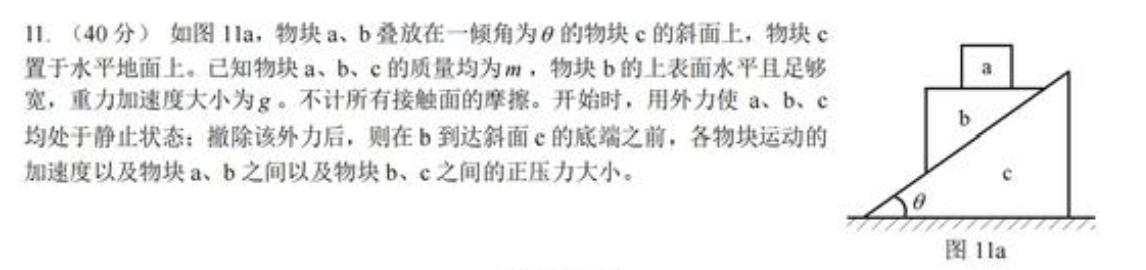
\includegraphics[width=1\textwidth]{image/image.png}
\end{center}

这道题完全打败了当时的我，我根本无从下手，这些复杂的受力和相对运动，我根本无法依靠我的直觉列出所有方程。而当我听了老师的讲解后我才知道，体系化的解法并非束缚，而是一种应万变于不变之法。要解决它我不需要劳费神思去想想它的运动，而只需要列出每一个物体的牛二方程：
\[
\begin{cases}
m\mathbf{a}_1= \mathbf{G}_c+\mathbf{N}_{bc},\\
m\mathbf{a}_2= \mathbf{G}_b+\mathbf{N}_{cb}+\mathbf{N}_{ab},\\
m\mathbf{a}_3= \mathbf{G}_a+\mathbf{N}_{ba}+\mathbf{N}.
\end{cases}
\]
之后我们便可以以列出的矢量方程式为纲要，列出各分量的分解形式：
\[
\begin{cases}
0 = 0 \\
mg - N_1 = ma_a
\end{cases}
\qquad
\begin{cases}
N_2 \sin\theta = ma_{b_{\text{水平}}} \\
mg + N_1 - N_2 \cos\theta = ma_{b_{\text{竖直}}}
\end{cases}
\qquad
\begin{cases}
N_2 \sin\theta = ma_c \\
N_{ground} - mg - N_2 \cos\theta = 0
\end{cases}
\]
我们观察到这里有五个方程和五个未知数：$a_a$，$a_c$，$a_b$，$N_1$，$N_2$。那么这个方程组可解，根据题目约束条件联立求解，可得各物理量如下：

\[
\left\{
\begin{aligned}
a_a &= a_{b_{\text{竖直}}}=\frac{4}{4+\cot^2\theta}g,\\
a_c &= a_{b_{\text{水平}}}=\frac{2}{4\tan\theta+\cot\theta}g,\\
a_b &= \frac{2g\tan\theta}{\sqrt{1+4\tan^2\theta}}.
\end{aligned}
\right.
\qquad
\left\{
\begin{aligned}
N_1 &= \frac{\cot^2\theta}{4+\cot^2\theta}mg,\\
N_2 &= \frac{2\cos\theta}{3\sin^2\theta+1}mg.
\end{aligned}
\right.
\]
这就十分轻而易举的得到我冥思苦想想不出来的答案了，多么优雅！

事实上这只是一个纯粹的力学问题，在后续的学习中我们还会遇到各种各样的约束，有的约束很好找，有的却要费点心思（比如动滑轮），但是力学部分实际建模时，常把问题归结为“几何约束 + 动力学方程 + 守恒/定理方程”的联立求解。常见形式如下：

\begin{enumerate}
\item \textbf{几何关系约束}
\[
f(x_1,x_2,\dots,t)=0.
\]
这一部分主要从长度、角度、接触条件三方面考虑。长度比如动滑轮，滑轮位移和重物位移常有固定比例关系；角度比如三角形三边满足余弦定理；接触条件对应物体不分离时法向相对速度与加速度约束。

\item \textbf{纯滚动约束方程}
\[
v_{\mathrm{cm}}=\omega R,
\qquad
a_{\mathrm{cm}}=\alpha R.
\]
这个约束只会在明确有滚动的情况下使用。

\item \textbf{牛顿第二定律约束方程}
\[
\sum \mathbf F=m\mathbf a,
\qquad
\text{分量式：}\sum F_x=ma_x,\;\sum F_y=ma_y.
\]
牛顿第二定律提供的力学约束是最多的，绝大多数质点问题都会用到这个方程。
\item \textbf{转动定律约束方程}
\[
\sum \boldsymbol\tau=\frac{\mathrm d\mathbf L}{\mathrm dt},
\qquad
\text{定轴刚体：}\sum \tau=I\alpha.
\]
这类约束只有在非质点或者质点系中才会用到，只要存在转动就要考虑力矩的约束了。
\item \textbf{动能定理-动量定律}
\[
\begin{cases}
\Delta T=W.    \\
\Delta \mathbf p=I.
\end{cases}
\]
这二者一般紧密联用，在没有耗散力的时候，动能定理也能用能量守恒等价替换。不过记住，存在转动的情况下动能包括平动动能和转动动能

\end{enumerate}

\newpage

\section{运动的方程的求解}

在初高中的物理学问题中，我们大多只局限于一维的直线运动，但是现实生活中更多是三维空间中的复杂曲线描述的运动，只运用一维方程无法描述。但好在得益于矢量的叠加性质，我们得以将三维空间中的复杂运动分解为三个一维运动方程，每一个方程描述了物体在各自坐标轴投影上的坐标随时间的函数，它们叠加起来就构成了物体复杂的运动轨迹，不过这轨迹本质上是一个点集，要把它切成曲线方程还要另费一番功夫，不过对于每一时刻下物体，我们引入\textbf{位矢$\mathbf{r} $}来描述它的空间位置，以方便我们对物体运动轨迹的描述
\[
\mathbf{r}(t)=x(t)\hat{\mathbf{i}}+y(t)\hat{\mathbf{j}}+z(t)\hat{\mathbf{k}}
\]
那么一维的运动理论就可以自然的推广到三维，所以速度和加速度就可以简单的表示为位矢的导数：
\[
\mathbf{v}(t)  =\frac{d\mathbf{r}(t)}{dt}
\qquad
\mathbf{a}(t)  =\frac{d\mathbf{v}(t)}{dt}
\]
当然直角坐标系它虽然是一个规范及标志的描述方式，但在物理学的绝大多数问题中，这三个垂直维度的描述却常常成为累赘，因为我们生存在三维空间，而能量的耗散因此多以球状弥散于空间中，所以绝大多数力场都是中心立场，顾名思义它们都有一个中心，数学表达式上带有$r^n$，而这半径在三维直角坐标系下的方程极复杂，但它又常常作为一个整体出现，为了寻求便捷以及对称性，我们常使用球坐标系描述力场的运动，这在后面会学习的电磁场，引力场中常常用到。

不过毕竟球坐标系的参量还是“过于繁复”，所以我们先介绍球坐标系，但道理是一样的。要转化为极坐标系也不算困难，首先需要注意到，不同以往，这次我们的求导对象需要被看成一个矢量，根据求导法则，结果应该写作：

\[
\frac{d\mathbf{r}(t)}{dt} = \frac{dr}{dt}\hat{\mathbf{r}} + \frac{d\hat{\mathbf{r}}}{dt}r
\]

在直线运动中$d\hat{\mathbf{r}}$项不随事件而变化，故并不影响什么，但在极坐标系中$d\hat{\mathbf{r}}$则随时间变化，比如在极坐标系中，其微分可以被证明为：
\[
d\hat{\mathbf{r}}= d{\theta} \hat{\mathbf{\theta}}
\]
所以速度项中常常带有$\omega$，但加速度会更加复杂，因为我们的$\hat{\mathbf{\theta}}$也是时间的函数，并且恰好是
\[
d\hat{\mathbf{r}}= -d{\theta} \hat{\mathbf{r}}
\]
这个其实画图就可以看出来，如果我记得补充图的话我会在这里为你们画一幅美丽的图像，如果我忘了就当我没说，你们自己画一画吧。总而言之，这二者的关系像极了正弦函数和余弦函数，导着导着就冒出个负号，如果你不记公式的话一定要小心处理，不过就正常的求导，我们便可以得到极坐标系的速度和加速度：

\[
\mathbf{v}=\dot r\,\hat{\mathbf r}+r\dot\theta\,\hat{\boldsymbol\theta}
\]
\[
\mathbf{a}=\left(\ddot r-r\dot\theta^{2}\right)\hat{\mathbf r}
+\left(r\ddot\theta+2\dot r\dot\theta\right)\hat{\boldsymbol\theta}
\]

其中第一项 \(\ddot r-r\dot\theta^2\) 是径向加速度，第二项 \(r\ddot\theta+2\dot r\dot\theta\) 是切向加速度；当 \(\dot r=0\) 且 \(\ddot\theta=0\) 时就退化为常见的向心加速度 \(-r\omega^2\hat{\mathbf r}\)，也就是说此时物体做圆周运动。



\subsection{力学约束的基石——牛顿三定律}

牛顿三定律构成了经典力学的基础，其内容可概括如下：

\begin{itemize}
\item \textbf{第一定律（惯性定律）}：当物体所受合外力为零时，物体保持静止状态或做匀速直线运动。
\[
\sum \mathbf{F}=0 \Rightarrow \mathbf{v}=\text{常量}
\]

\item \textbf{第二定律（动力学基本定律）}：物体的加速度与所受合外力成正比，与质量成反比，加速度方向与合外力方向一致。
\[
\sum \mathbf{F}=m\mathbf{a}
\]

\item \textbf{第三定律（作用与反作用定律）}：两个物体之间的作用力与反作用力大小相等、方向相反，并作用在不同物体上。
\[
\mathbf{F}_{AB}=-\mathbf{F}_{BA}
\]
\end{itemize}

在处理实际问题时，通常先进行受力分析，列出平衡方程，之后再结合几何约束与边界条件求解。这部分其实有用的也就是个牛顿方程会给出约束条件，其它的在经典力学都是作为公理存在的。为了更好的说明牛顿定律在静力学平衡中不可逾越的地位，我们来看这道来自第41届全国中学生物理竞赛预赛的题目：

\begin{center}
    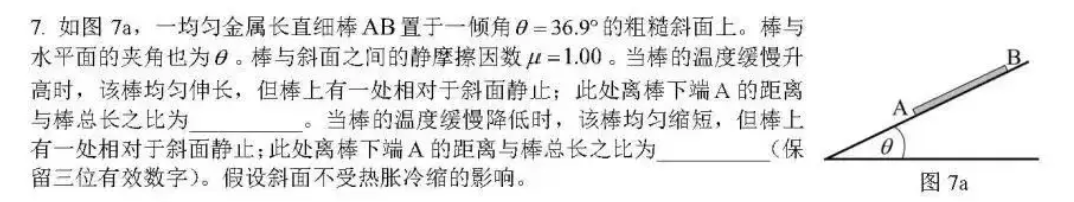
\includegraphics[width=1\textwidth]{image/eg2.png}
\end{center}

我们很清楚，静止的点一定受力平衡，所以我们一定想列出膨胀和冷却时候的受力方程。在这里我给出诚恳的建议：一定要提前取正方向，不然在计算的时候会被正负号搞得头大。我们设沿斜面向上为正方向，$x$ 为 $PA$ 的长度。既然 $P$ 点是相对斜面静止的点，它两侧的棒段就必然存在相对滑动的趋势。为了找准摩擦力和内力的方向，我们可以把棒在 $P$ 点处物理上断开，分别对 $PA$ 段和 $PB$ 段进行隔离受力分析：

\begin{gather*}
\begin{cases}
\displaystyle T_A + f_A + G_A = 0 & \text{（$PA$段平衡 ）} \\[8pt]
\displaystyle f_A = G_A  & \text{（最大静摩擦）}
\end{cases}
\qquad
\begin{cases}
\displaystyle T_B + f_B + G_B = 0 & \text{（$PB$段平衡 ）} \\[8pt]
\displaystyle f_B = G_B  & \text{（最大静摩擦）}
\end{cases}
\end{gather*}

以 $P$ 为参考，$PA$ 段各点相对斜面有向下滑动的趋势，故 $PA$ 段受到的静摩擦力 $f_A$ 沿斜面向上（正方向）；$PB$ 段各点相对斜面有向上滑动的趋势，故 $PB$ 段受到的静摩擦力 $f_B$ 沿斜面向下（负方向）。设 $P$ 点处 $PB$ 对 $PA$ 的作用力为 $T$（沿斜面向上为正），则 $PA$ 对 $PB$ 的作用力为 $-T$。

温度升高（均匀伸长）时$PA$ 段相对斜面有下滑趋势，摩擦力 $f_A$ 沿斜面向上；$PB$ 段有上滑趋势，摩擦力 $f_B$ 沿斜面向下。设 $PB$ 对 $PA$ 的内力为 $T$（沿斜面向上为正），则：

\begin{gather*}
\begin{cases}
\displaystyle T + f_A - mg\frac{x}{L}\sin\theta = 0 & \text{（$PA$段平衡 ）} \\[8pt]
\displaystyle f_A = \mu \cdot mg\frac{x}{L}\cos\theta  & \text{（最大静摩擦）}
\end{cases}
\qquad
\begin{cases}
\displaystyle -T - f_B - mg\frac{L-x}{L}\sin\theta = 0 & \text{（$PB$段平衡 ）} \\[8pt]
\displaystyle f_B = \mu \cdot mg\frac{L-x}{L}\cos\theta  & \text{（最大静摩擦）}
\end{cases}
\end{gather*}

由第一组方程解出 $T$，代入第二组，整理得：

\[
2x\cos\theta = L(\sin\theta + \cos\theta)
\]

于是：

\[
\boxed{\frac{x}{L} = \frac{\sin\theta + \cos\theta}{2\cos\theta} = \frac{1 + \tan\theta}{2} = \frac{1 + 0.75}{2} = \frac{7}{8} = 0.875}
\]

\textbf{温度降低（均匀缩短）}时滑动趋势相反：$PA$ 段有上滑趋势，摩擦力向下；$PB$ 段有下滑趋势，摩擦力向上。

\begin{gather*}
\begin{cases}
\displaystyle T - f_A - mg\frac{x}{L}\sin\theta = 0 & \text{（$PA$ 段平衡）} \\[8pt]
\displaystyle f_A = mg\frac{x}{L}\cos\theta & \text{（最大静摩擦）}
\end{cases}
\qquad
\begin{cases}
\displaystyle -T + f_B - mg\frac{L-x}{L}\sin\theta = 0 & \text{（$PB$ 段平衡）} \\[8pt]
\displaystyle f_B = mg\frac{L-x}{L}\cos\theta & \text{（最大静摩擦）}
\end{cases}
\end{gather*}

联立解得：

\[
\boxed{\frac{x}{L} = \frac{\cos\theta - \sin\theta}{2\cos\theta} = \frac{1 - \tan\theta}{2} = \frac{1 - 0.75}{2} = \frac{1}{8} = 0.125}
\]

\textbf{总结：} 这道题的关键在于正确判断热胀冷缩时各段的相对滑动趋势，从而确定静摩擦力的方向。通过隔离 $PA$ 和 $PB$ 两段，分别列写沿斜面方向的平衡方程，利用 $P$ 点处内力大小相等、方向相反（牛顿第三定律）将两方程联立，即可消去未知内力 $T$，直接得到关于 $x/L$ 的简洁方程。温度升高时静止点距 $A$ 为 $0.875L$，温度降低时为 $0.125L$，两者恰好关于棒的中点对称，这正是物理对称性的体现。



\subsection{刚体和质点系的转动}

当我们的运算对象不能被是做质点的时候，力的作用位点往往也会影响力的作用效果，我们在玩弄一个木棍的时候，总是存在一个平衡点，当我们作用一个数值向上的力在那个平衡点的时候，木棍就静止在手上了，但只要我们偏移一点，木棍就会开始旋转，然后掉在地上。说明即使对于一个不能被视作质点的物体，它总有一个点起到了类似质点的作用，这一点我们就叫作质心，作用在质心上的力等效于作用于等效的质点的力的效果，对于任意图形，我们都可以视作无数质量微元组成的离散体系。

但是怎么求这离散体系的质心呢？我们现有的平动数学工具是无法解决的。但是我们知道只有当力作用于偏离质点的一个位置才会导致旋转，也就是导致旋转的量一定是和半径有关的，这一瞬间木棍一定是经历了一个角加速的。类似平动问题，我们可以写出转动问题的位矢，速度和加速度的对应关系：
\[
\mathbf r\leftrightarrow \boldsymbol\theta,\qquad
\mathbf v\leftrightarrow \boldsymbol\omega,\qquad
\mathbf a\leftrightarrow \boldsymbol\alpha,
\]
其中 \(\boldsymbol\omega\) 为角速度，\(\boldsymbol\alpha\) 为角加速度。我们不难发现，这几个量和平动力学的唯一区别差了一个长度的因子。而是这个因子让我们统一了刚体各点的速度，对于一个刚体而言，各点的角速度，角加速度相等。

回到那个木棍，既然作用于质心的力不改变其转动情况，那么我们先让质心在动力场下平衡，也就是让它作为一个支点，这听起来十分耳熟不是？没错这就是阿基米德的杠杆定律！但注意，这时候杠杆定律考虑的力一定是垂直于力的作用臂的，那么不垂直呢？没错平行于木棍的力的分量会导致木棍的水平平动，所以其实只有垂直于木棍的力会影响，我们可以把它写成矢量式，定义这个力对应的量为力矩，力对参考点 \(O\) 的力矩定义为
\[
\boldsymbol\tau_O=\mathbf r\times \mathbf F.
\]
力臂不随时间改变，所以力矩也对应有角动量，质点对同一点的角动量为
\[
\mathbf L_O=\mathbf r\times \mathbf p=\mathbf r\times m\mathbf v.
\]
对固定惯性参考点可得角动量定理
\[
\frac{\mathrm d\mathbf L_O}{\mathrm dt}=\sum \boldsymbol\tau_O^{\,\text{ext}}.
\]
于是刚刚的木棍的问题就可以转化成一个力矩平衡的问题了，只有力矩平衡的时候刚体才不会发生转动，而作用于质心的力矩为0，所以它指向任意方向都只会导致平动。此外当外力矩为零时，\(\mathbf L_O\) 守恒。这在许多中心力场问题中作为重要的守恒量出现，给出一个方程。

这时候我们或许就可以求解质心了，我们知道质心是力矩平衡点，将木棍写成一个一维坐标系，我们可以假设质心为$x_c$，那么力矩平衡的方程就是：
\[
 \sum_i (x_i-x_c) F_i=0.
\]
但是这里面仍然有未知项，我们没办法解决，但毕竟又不是实际问题，我们自己加一点约束就好了，我们可以假定作用力大小都一样，或者更方便得，假设它反比于到原点的距离，但如论如何我们都可以移项得到：
\[
 \sum_i x_i F_i=\sum_i x_c F_i.
\]
这说明质心也意味着力矩等效点，对每个质量微元的作用力的效果可以统一到质心，对于一个刚体，必然有角加速度一样，这样就可以得到离散体系质心定义：
\[
\mathbf R_{\mathrm{cm}}=\frac1M\sum_i m_i\mathbf r_i,
\qquad M=\sum_i m_i.
\]
或者写成连续体的积分形式：
\[
\mathbf R_{\mathrm{cm}}=\frac1M\int \mathbf r\,\mathrm dm.
\]

诶这时候我们发现，出现了一个类质量项$m_i\mathbf r_i$，显然它才是决定力作用效果的一个东西，它起到一个什么作用？同样的力，它越大，作用效果越弱，诶！这听起来是不是很想惯性的定义，没错它就是转动惯量，对绕固定轴 \(z\) 转动的刚体，定义转动惯量：
\[
I_z=\sum_i m_i r_{i\perp}^2\quad (\text{连续体 }I_z=\int r_\perp^2\,\mathrm dm).
\]

\begin{table}[htbp]
\centering
\renewcommand{\arraystretch}{1.5}
\begin{tabular*}{\textwidth}{@{\extracolsep{\fill}}lll}
\toprule
物体 & 转轴 & 转动惯量 \\
\midrule
细棍（长度 $L$，质量 $M$） & 过中心且垂直棍 & $I=\dfrac{1}{12}ML^2$ \\
细棍（长度 $L$，质量 $M$） & 过端点且垂直棍 & $I=\dfrac{1}{3}ML^2$ \\
长方形薄板（边长 $a\times b$，质量 $M$） & 过中心且垂直板面 & $I=\dfrac{1}{12}M(a^2+b^2)$ \\
实心圆盘（半径 $R$，质量 $M$） & 过中心且垂直盘面 & $I=\dfrac{1}{2}MR^2$ \\
实心球（半径 $R$，质量 $M$） & 过球心任一直径 & $I=\dfrac{2}{5}MR^2$ \\
\bottomrule
\end{tabular*}
\end{table}
转动惯量就是转动力学中的质量，有了它我们就可以把相应等式改写为；

\[
\underbrace{\mathbf p=m\mathbf v}_{\text{动量，力和质量}}
\quad\Longleftrightarrow\quad
\underbrace{\mathbf L=\mathbf I\boldsymbol\omega}_{\text{角动量，力矩和转动惯量}}
\]
\[
\underbrace{\mathbf F=\frac{\mathrm d\mathbf p}{\mathrm dt}=m\mathbf a}_{\text{平动牛顿第二定律}}
\quad\Longleftrightarrow\quad
\underbrace{\boldsymbol\tau=\frac{\mathrm d\mathbf L}{\mathrm dt}=\mathbf I\boldsymbol\alpha}_{\text{转动对应形式（定轴）}}
\]


这样我们就解决了绝大多数理想情况下的转动问题了，但是有时候转动的支店并不一定选在中点或者端点的位置，我们在解这类问题时候想必不会希望每次都积分吧，所以我们有两种转动惯量定理，分别解决了支点水平移动和垂直叠加的情况。

第一个是平行轴定理（Steiner 定理）：若已知过质心轴的转动惯量 \(I_{\mathrm{c}}\)，则与其平行、相距 \(d\) 的轴的转动惯量满足
\[
I=I_{\mathrm{c}}+Md^2.
\]
有了这个公式，当我们在计算支点在小木棍四分之一处的时候的问题就很简单了，就是质心的转动惯量（中点）再加上个系数。

第二个是垂直轴定理：
\[
I_z=I_x+I_y.
\]
利用这个公式在计算二维平面的转动惯量的时候可能会更加方便，比如长方形薄板。

\subsubsection{质点系与内力矩}

转动体系是对于无法看成单质点的物体，但是我们可以将这样的物体看成质点系。把刚体或多粒子系统看成由若干质点组成的质点系后，角动量定理可写成
\[
\frac{\mathrm d\mathbf L_O}{\mathrm dt}=\sum \boldsymbol\tau_O^{\,\text{ext}}+\sum \boldsymbol\tau_O^{\,\text{int}}.
\]
其中外力矩决定系统与外界的角动量交换，内力矩描述系统内部相互作用对总角动量的影响。这个式子就是转动力学的牛顿第二定律。
对任意一对内力（第 $i,j$ 个质点）有
\[
\mathbf F_{ij}=-\mathbf F_{ji},
\]
其对应内力矩和为
\[
\boldsymbol\tau_{ij}+\boldsymbol\tau_{ji}=(\mathbf r_i-\mathbf r_j)\times \mathbf F_{ij}=0.
\]

从而总内力矩为零，此时质点系总角动量演化只由外力矩决定：
\[
\frac{\mathrm d\mathbf L_O}{\mathrm dt}=\sum \boldsymbol\tau_O^{\,\text{ext}}
\]
特别地，当外力矩也为零时，质点系总角动量守恒。

这个结论在碰撞、天体两体问题、以及“内力很大但不改变系统总角动量”的分析中非常关键。也就是这个推论才允许我们在中心力场问题中使用角动量守恒这一重要的约束条件。


当然对于刚体运动，这种单线程的方程就已经可以解决绝大多数问题了，但是总有混沌系统，比如流体力学中的各种东西，它是互相耦合的，所以这时候我们常常使用张量表示，也就是矩阵：
\[
\mathbf L=\mathbf I\,\boldsymbol\omega,
\]
其中 \(\mathbf I\) 为惯性张量。在主轴系中 \(\mathbf I\) 对角化，分量形式为
\[
L_i=I_i\omega_i\qquad (i=1,2,3).
\]

\subsection{功和能}

在初中我们就知道有一个叫功的定义：
\[
W=\mathbf F\cdot\Delta\mathbf r=F\,\Delta r\cos\theta.
\]
这是一个离散化的表达，事实上所有的定理都是先定义简单情况的离散表示，将位移变化量写成位移微元，将投影写成向量的点积，我们便将这个一维离散化的表达式写成三维连续的表达式：
\[
W=\int_{C}\mathbf F\cdot d\mathbf r.
\]
这有什么用呢？我们展开来看看：
\[
dW=\mathbf F\cdot d\mathbf r=md\mathbf{v} \cdot \frac{d\mathbf r}{dt}=md\mathbf{v} \cdot \mathbf{v}=d(\frac12 mv^2) .
\]
诶我们就发现，做功等价于一个只与质量速度有关的量，这个我们称之为动能，顾名思义就是物体运动所蕴含的能量，为了与分析力学相容我们一般使用符号$T$表示，根据我们的推导不难看出合外力做功转化为动能，诶，那你也许会想到啊这就是对牛二方程进行了一个路径积分嘛，没错，这样得到的结果就是动能定理：
\[
\Delta T = \sum W_i
\]
也就是说动能变化等于各分力做功之和，这一版和动能定理联用给出速度约束方程。

那么这些$W_i$都包含些什么呢？想想我们日常里的力：摩擦力，万有引力，电磁力，阻力...。这些力要么只与坐标有关，要么与压力有关，要么与速度有关看样子很难分类，不过我们仍然可以粗犷的分为两大类：位置有关力和位置无关力。在物理学中一般也成为保守力和非保守力。


\begin{itemize}
\item 保守力，比如万有引力，电磁力，都满足平方二次反比的关系，这与场的球状耗散有关，它们都存在势能函数 $U$，满足
\[
\mathbf F=-\nabla U,
\qquad
W_{\text{cons}}=-\Delta U.
\]
常见保守力有电磁力，万有引力和弹力。其中前二者都是平方反比的，而弹力则是正比于位置的二次方的。

\item 非保守力，比如摩擦力，空气阻力，都是做功只与运动路程有关的力，它们的功一般都标识着能量的耗散
\end{itemize}

显然除了非保守力功是无法预测的，保守力功和动能都只需要知道物体的始末状态就可以确定的了，而不需要知道过程中任何其它信息。所以我们将这两种能量合在一起称作机械能：
\[
E=T+U.
\]

其中动能项，一般而言，对于非质点物体，都具有平动动能和转动动能，转动动能也就是将平动动能作了一个映射，它是由质心速度和相对质心的转动惯量描述：
\[
T=\frac12 M V_{\mathrm{cm}}^2+\frac12 I_{\mathrm{cm}}\omega^2,
\]
在惯性系间转换参考系不改变这一等式，但是转化为非惯性系时需要计入惯性力修正。

当系统没有外力的时候，我们就可以称其机械能守恒，这也可以提供一个等价于动能定理的约束。

\subsection{力学模型}

前面讲了那么多定律、约束和守恒量，如果最后不能落到几个活生生的模型上，那些公式就还是像挂在墙上的工具，看得见，却没有真正拿在手里用过。所以这里不妨一口气看三个经典例子：一个告诉我们阻力怎样悄悄改写最熟悉的抛体运动，一个告诉我们为什么天体轨道总喜欢画出圆锥曲线，另一个则告诉我们陀螺为什么偏偏不朝着力矩方向倒下去。

\subsubsection{平抛运动的数学模型}

先看平抛。若没有空气阻力，这几乎是中学里最“听话”的运动之一：水平方向匀速，竖直方向匀加速，彼此互不干扰。可一旦空气开始拉扯这个物体，事情就不再那么整齐了。为了不把问题弄得太凶，我们取最常见的线性阻力模型，设质量为$m$的质点在$x$--$y$平面内运动，$x$轴水平向右，$y$轴竖直向上，重力加速度为$g$，阻力满足
\[
\mathbf{F}_d=-k\mathbf{v}
\]
其中$k>0$为阻力系数。这个式子很朴素，它只是在说：物体跑得越快，空气越不愿意让它跑。于是牛顿第二定律立刻给出两个方向上的方程
\[
\begin{cases}
m\dfrac{dv_x}{dt}=-k v_x,\\[4pt]
m\dfrac{dv_y}{dt}=-mg-k v_y.
\end{cases}
\]
如果初始条件取为
\[
x(0)=0,\quad y(0)=0,\quad v_x(0)=v_0\cos\theta,\quad v_y(0)=v_0\sin\theta,
\]
那么这组方程其实很老实，因为两个分量已经分开了。积分之后，速度随时间的变化是
\[
v_x(t)=v_0\cos\theta\,e^{-\frac{k}{m}t},
\]
\[
v_y(t)=\left(v_0\sin\theta+\frac{mg}{k}\right)e^{-\frac{k}{m}t}-\frac{mg}{k}.
\]
你一眼就能看出这里发生了什么：水平方向的速度被指数地磨掉，竖直方向则一边被重力往下拽，一边被阻力往回拉，最后不再无限增大，而是慢慢逼近某个极限下落速度。再往下积一次，位置便是
\[
x(t)=\frac{m v_0\cos\theta}{k}\left(1-e^{-\frac{k}{m}t}\right),
\]
\[
y(t)=\frac{m}{k}\left(v_0\sin\theta+\frac{mg}{k}\right)\left(1-e^{-\frac{k}{m}t}\right)-\frac{mg}{k}t.
\]
这几个式子看着比无阻力情形笨重得多，可它们告诉我们的图像却很清楚：真实世界里的抛体，从来不是一条完美的抛物线，它总要在空气里一点点“泄气”，飞得没那么远，也落得没那么倔强。

\subsubsection{天体的运行的原理}

接着把目光从地面抬到天上。中心力场的问题乍看很复杂，因为物体一边绕着中心转，一边离中心远近变化，好像每时每刻都在拧着走。但自然在这里给了我们一个极大的恩惠：只要力始终沿着径向，也就是
\[
\mathbf F(r)=F(r)\hat{\mathbf r},
\]
那么力矩就自动消失，角动量守恒便立刻成立：
\[
L=m r^2\dot\theta=\text{常量}.
\]
这句话的分量不多，内容却很多。它首先告诉我们，运动一定被压在某个平面里；其次它还暗示，与其直接去求$r(t)$和$\theta(t)$，不如换个更聪明的变量。令 \(u(\theta)=1/r\)，便可把牛顿方程整理成著名的 Binet 方程
\[
\frac{\mathrm d^2u}{\mathrm d\theta^2}+u=-\frac{m}{L^2u^2}F\!\left(\frac1u\right).
\]
这一步看上去像是数学上的花招，其实是在顺着问题本身的对称性思考。特别地，当力取平方反比形式
\[
F(r)=-\frac{k}{r^2}\quad (k>0),
\]
也就是万有引力和库仑力最核心的那个样子时，方程忽然一下子变得温顺起来：
\[
\frac{\mathrm d^2u}{\mathrm d\theta^2}+u=\frac{mk}{L^2}.
\]
这已经是我们最熟悉的常系数线性方程了，因此其解自然写成
\[
u(\theta)=\frac{mk}{L^2}\bigl(1+e\cos(\theta-\theta_0)\bigr).
\]
把它翻回到$r$，轨道方程就是
\[
r(\theta)=\frac{p}{1+e\cos(\theta-\theta_0)},
\qquad
p=\frac{L^2}{mk}.
\]
这时候一个很美的事实就出现了：那些我们在几何课上见过的椭圆、抛物线和双曲线，并不是数学家凭空想出来的图形，它们竟然就是自然界里中心力运动的真实轨道。参数 \(e\) 叫离心率，而它几乎一手包办了轨道的性格：\(0\le e<1\) 时是椭圆，\(e=1\) 时是抛物线，\(e>1\) 时是双曲线。于是开普勒的行星轨道、彗星的一去不返、散射问题中的偏折路径，都在这个式子里悄悄统一了。

\subsubsection{陀螺的进动}

最后来看陀螺。它最迷人的地方在于，它总做出一种与直觉作对的举动。你明明看见重力在拽它，按平常经验它该顺着力矩方向倒下去；可它偏偏不急着倒，而是绕着竖直方向慢慢转圈。这里面真正“顽固”的不是陀螺，而是它原本已经很大的角动量。设刚体绕对称轴自旋角速度为 \(\omega\)，支点到质心距离为 \(l\)，倾角为 \(\theta\)，那么重力对支点的力矩大小为
\[
\tau = mgl\sin\theta.
\]
角动量定理仍然写成
\[
\frac{\mathrm d\mathbf L}{\mathrm dt}=\boldsymbol\tau.
\]
但这一次，我们最该注意的不是大小，而是方向：在快速自旋近似下，\(\mathbf L\) 的长度几乎不怎么变，真正变化的是它的指向。若陀螺以进动角速度 \(\Omega_p\) 绕竖直轴缓慢转动，那么几何上有
\[
\left|\frac{\mathrm d\mathbf L}{\mathrm dt}\right|=\Omega_p L\sin\theta.
\]
与力矩大小比较，便得到
\[
\Omega_p=\frac{\tau}{L\sin\theta}=\frac{mgl}{L}.
\]
如果进一步利用高速自旋时的近似 \(L\approx I_3\omega\)（这里 \(I_3\) 是对称轴的转动惯量），就有
\[
\Omega_p\approx\frac{mgl}{I_3\omega}.
\]
这个结果简直像一句带点讽刺意味的话：你转得越快，反而越不容易立刻倒下；重力越大、质心抬得越高，它绕圈的速度才越快。也就是说，力矩并没有直接把陀螺摁倒，它只是不断地拽着角动量的方向，让它沿着旁边绕开。理解了这一点，陀螺、陀螺仪，乃至许多姿态稳定问题，其实都不再神秘；它们不过是在提醒我们，转动的世界和直线运动一样服从牛顿定律，只是那里的“倔强”不写在速度里，而写在角动量里。


\newpage
\section{统计力学}

描述一个具有随机行为的系统，就需要统计力学，统计力学的基础则是概率论，在我们生活中存在许多随机系统，比如分子运动，流体，都是存在诸多偶发行为的，无法预测的系统，而统计力学给我们描述这种系统的基础。

在概率学的框架下，概率由概率空间 $(\Omega,\mathcal{F},\mathbb{P})$ 描述：$\Omega$ 为样本空间，$\mathcal{F}$ 为事件 $\sigma$-代数，$\mathbb{P}:\mathcal{F}\to[0,1]$ 为概率测度，满足
\[
\mathbb{P}(\Omega)=1,
\qquad
\mathbb{P}\!\left(\bigcup_{i=1}^{\infty}A_i\right)=\sum_{i=1}^{\infty}\mathbb{P}(A_i)
\]
（其中 $A_i$ 两两不交）。这就是概率学语言下的概率计算，这时候概率被视作一个函数，将事件映射为概率。

描述事件的重要参数是随机变量，随机变量可视为可测映射 $X:\Omega\to\mathbb{R}$，它满足
\[
f(x) \ge 0,\qquad \int_{-\infty}^{+\infty} f(x)\,\mathrm{d}x = 1.
\]

区间概率由概率密度对随机变量的积分给出：
\[
P(a\le X\le b)=\int_a^b f(x)\,\mathrm{d}x.
\]

期望可先用测度形式写为
\[
\mathbb{E}[X]=\int_{\Omega}X(\omega)\,\mathrm{d}\mathbb{P}(\omega)=\int_{\mathbb{R}}x\,\mu_X(\mathrm{d}x).
\]

当密度 $f$ 存在时，上式化为常见积分形式。常用统计量包括期望与方差：
\[
\mathbb{E}[X]=\int_{-\infty}^{+\infty}x f(x)\,\mathrm{d}x,
\qquad
\mathrm{Var}(X)=\mathbb{E}\!\left[(X-\mathbb{E}[X])^2\right].
\]

在热平衡近似下，许多宏观可观测量会接近高斯分布
\[
f(x)=\frac{1}{\sqrt{2\pi\sigma^2}}\exp\!\left[-\frac{(x-\mu)^2}{2\sigma^2}\right],
\]
其中 $\mu$ 为均值、$\sigma^2$ 为方差。该形式与中心极限定理密切相关，是统计力学中涨落分析的基础模型之一。

不过这部分内容我们后面根本用不到。这部分内容是我在听一个学长讲统计力学的时候听到的，他讲了一节课枯燥乏味的定理，我想他是数学系的，不然为什么会这么严谨呢？所以我把它留在这，不然数学系的会不开心的。

热力学最初是从经验定律出发建立的：温度、压强、体积、热量、内能这些宏观量之间满足稳定的实验关系。但统计力学告诉我们，这些宏观规律并不是凭空出现的，而是大量微观粒子运动的集体平均结果。换句话说，\textbf{热力学是统计力学在宏观极限下的表现}。

设一个系统由大量粒子组成。若只给出总能量、体积、粒子数等少量宏观参量，我们所描述的是\textbf{宏观态}；而若给出每个粒子的位置与动量，则描述的是\textbf{微观态}。同一个宏观态往往对应海量不同的微观态。

统计力学的核心思想是：在热平衡时，系统最可能处于那些对应微观态数最多的宏观态，这也是熵增定律的数学体现。于是我们引入熵：
\[
S=k_{\mathrm B}\ln \Omega,
\]
其中 \(\Omega\) 表示在给定约束下可实现的微观态数，它是一个纯粹的统计学数据，因而数目常常大得无法想象，\(k_{\mathrm B}\) 为玻尔兹曼常数。这个式子把“无序程度”精确地转化为“微观态计数”的对数。

如果两个系统可以交换能量，总系统会自发演化到总微观态数最大的状态，也就是总熵最大的状态。对总熵全微分展开可以得到：
\[
\mathrm dS=\left(\frac{\partial S}{\partial U}\right)_{V,N}\mathrm dU+\left(\frac{\partial S}{\partial V}\right)_{U,N}\mathrm dV+\left(\frac{\partial S}{\partial N}\right)_{U,V}\mathrm dN.
\]

我们知道热力学第一定律的具体形式是：
\[
 U= \delta Q + \delta W
\]

现在我们来将其写成微分形式，按照高中学习的求导法则我们对每一项取微分，这里因为我们考虑的压力环境不是大气压下，所以压强也是变量，所以我们得到：
\[
\mathrm dU=T\,\mathrm dS-P\,\mathrm dV+\mu\,\mathrm dN.
\]
对照后可定义热力学变量
\[
\frac{1}{T}=\left(\frac{\partial S}{\partial U}\right)_{V,N},
\qquad
\frac{P}{T}=\left(\frac{\partial S}{\partial V}\right)_{U,N},
\qquad
-\frac{\mu}{T}=\left(\frac{\partial S}{\partial N}\right)_{U,V}.
\]

这说明温度、压强和化学势本质上都是熵对不同宏观约束的导数。

但是这并非描述本质的公式，为了建立可以直接描述围观的语言，我们需要采用一点数学方法——系综。

当系统与温度固定的热库接触时，系统可以和外界交换能量，但粒子数与体积保持不变，这就是正则系综。此时我们并不预先知道某个能级 \(E_i\) 的概率分布，而是要从“在给定平均能量约束下，哪一个概率分布最可能出现”这个问题出发去推导它。

要描述一个混沌系统不可能通过有限的式子描述，因为你不可能用有限描述无限。我们将一个系统以能量为随机变量测概率。设系统处于各能级 \(E_i\) 的概率为 \(P_i\)。这些概率首先满足归一化条件
\[
\sum_i P_i=1,
\]
同时系统的平均能量固定为
\[
\sum_i P_i E_i=U.
\]
在这两个约束下，平衡态应使信息熵，也就是信息量的“期望值”，也就是（这个公式其实就是波尔兹曼公式的简单变形）
\[
S=-k_{\mathrm B}\sum_i P_i\ln P_i
\]
取极大值。用拉格朗日乘子法，令
\[
\Phi=-k_{\mathrm B}\sum_i P_i\ln P_i-\alpha\left(\sum_i P_i-1\right)-\gamma\left(\sum_i P_iE_i-U\right).
\]
对每个 \(P_i\) 求偏导并令其为零：
\[
\frac{\partial \Phi}{\partial P_i}=-k_{\mathrm B}(\ln P_i+1)-\alpha-\gamma E_i=0.
\]
整理得
\[
P_i=\exp\left(-1-\frac{\alpha}{k_{\mathrm B}}\right)\exp\left(-\frac{\gamma}{k_{\mathrm B}}E_i\right).
\]
可见平衡分布必然是关于能量的指数分布。把前面的归一化常数记为 \(1/Z\)，并定义
\[
\beta\equiv \frac{\gamma}{k_{\mathrm B}},
\]
就得到
\[
P_i=\frac{e^{-\beta E_i}}{Z},
\qquad
Z=\sum_i e^{-\beta E_i}.
\]
这就是玻尔兹曼分布，而
\[
Z=\sum_i e^{-\beta E_i}
\]
就称为\textbf{配分函数}。它本质上是归一化条件所引入的“总权重和”，同时也编码了体系全部的平衡热力学信息。

但是这个表达式中还存在一个未知数 \(\beta\)，接下面说明 \(\beta\) 的具体含义。由上式可计算熵：
\[
S=-k_{\mathrm B}\sum_i P_i\ln P_i
=-k_{\mathrm B}\sum_i P_i(-\beta E_i-\ln Z)
=k_{\mathrm B}(\beta U+\ln Z).
\]
把它看成平均能量 \(U\) 的函数，我们之前提及过，在 \(V,N\) 固定时有热力学定义
\[
\left(\frac{\partial S}{\partial U}\right)_{V,N}=\frac{1}{T}.
\]
另一方面，从统计表达式出发可得
\[
\left(\frac{\partial S}{\partial U}\right)_{V,N}=k_{\mathrm B}\beta.
\]
两式对比立刻得到
\[
\beta=\frac{1}{k_{\mathrm B}T}.
\]
所以 \(\beta\) 并不是人为硬塞进去的记号，而是“熵对能量导数”这个热力学量在统计分布中的自然表现。温度越高，\(\beta\) 越小，高能级的指数压制越弱；温度越低，\(\beta\) 越大，系统越集中在低能态。

一旦得到了配分函数，其他热力学量也都可以从它推出。例如
\[
U=\sum_i P_iE_i=-\frac{\partial}{\partial \beta}\ln Z,
\]
进一步定义自由能
\[
F=U-TS=-k_{\mathrm B}T\ln Z,
\]
于是熵、压强和热容分别满足
\[
S=-\left(\frac{\partial F}{\partial T}\right)_{V,N},
\qquad
P=-\left(\frac{\partial F}{\partial V}\right)_{T,N},
\qquad
C_V=\left(\frac{\partial U}{\partial T}\right)_{V,N}.
\]

所以配分函数并不是凭空定义出来的技巧，而是由“最大熵原理 + 平均能量约束”自然推出的核心对象；而 \(\beta\) 与温度的关系，则来自统计熵定义与热力学温度定义之间的严格对应。

正因为配分函数拥有这样优美的性质，它也被成为统计力学的基本原理。在接下来的许多推导中我们都会或多或少的使用到它。

\subsection{理想气体状态方程的统计推导}

对单原子经典理想气体，单粒子哈密顿量只有平动动能：
\[
\varepsilon=\frac{p^2}{2m}.
\]
单粒子配分函数为
\[
Z_1=\frac{1}{h^3}\int e^{-\beta p^2/2m}\,\mathrm d^3p\,\mathrm d^3q.
\]
其中位置积分直接给出体积因子 \(V\)：
\[
\int \mathrm d^3q=V.
\]
动量积分是高斯积分：
\[
\int e^{-\beta p^2/2m}\,\mathrm d^3p=
\left(\int_{-\infty}^{+\infty}e^{-\beta p_x^2/2m}\,\mathrm dp_x\right)^3
=\left(\frac{2\pi m}{\beta}\right)^{3/2}.
\]
故
\[
Z_1=\frac{V}{h^3}(2\pi mk_{\mathrm B}T)^{3/2}.
\]

对 \(N\) 个不可分辨粒子，
\[
Z_N=\frac{Z_1^N}{N!}.
\]
于是自由能
\[
F=-k_{\mathrm B}T\ln Z_N.
\]
对体积求偏导得压强
\[
P=-\left(\frac{\partial F}{\partial V}\right)_{T,N}
=\frac{Nk_{\mathrm B}T}{V}.
\]
即
\[
PV=Nk_{\mathrm B}T=nRT.
\]
这就是理想气体状态方程。它表明压强与温度成正比、与粒子数密度 \(N/V\) 成正比。这里的比例系数不是拍脑袋写下的，而是来自配分函数中位置积分对体积的线性依赖。

上面的理想气体推导把体积 \(V\) 看成粒子位置可以取值的空间范围，但如果继续追问“为什么气体一定要占据一个有限体积，而不是所有分子都挤在一起”，就必须回到分子间相互作用的微观图像。

从微观上看，分子之间并不是完全“互不理睬”的。即使在电中性分子之间，也普遍存在由瞬时偶极、诱导偶极等效应产生的\textbf{范德瓦尔斯相互作用}。在较大距离上，这种吸引常可近似写成
\[
U_{\mathrm{att}}(r)\approx -\frac{C}{r^6},
\qquad C>0,
\]
其对应的径向力为
\[
F_{\mathrm{att}}(r)=-\frac{\mathrm dU}{\mathrm dr}=-\frac{6C}{r^7}.
\]
负号表示这是一种吸引力：当两个分子相距较远时，它们会倾向于彼此靠近。

但分子又不可能无限接近。因为当电子云开始明显重叠时，会出现非常强的短程排斥，这既可理解为库仑排斥，也可理解为泡利不相容原理在有效势中的体现。常用的经验势能模型是 Lennard--Jones 势：
\[
U(r)=4\varepsilon\left[\left(\frac{\sigma}{r}\right)^{12}-\left(\frac{\sigma}{r}\right)^6\right].
\]
其中 \(r\) 为分子间距，\(\varepsilon\) 表示势阱深度，\(\sigma\) 表示相互作用尺度。它对应的力为
\[
F(r)=-\frac{\mathrm dU}{\mathrm dr}
=\frac{24\varepsilon}{r}\left[2\left(\frac{\sigma}{r}\right)^{12}-\left(\frac{\sigma}{r}\right)^6\right].
\]
当 \(r\) 很大时，\(r^{-6}\) 项占主导，表现为吸引；当 \(r\) 很小时，\(r^{-12}\) 项迅速增大，表现为强排斥。

因此分子间通常存在一个平衡距离 \(r_0\)，满足
\[
F(r_0)=0
\qquad\Longrightarrow\qquad
r_0=2^{1/6}\sigma.
\]
这说明两个分子既不会无限远离，也不会塌缩到同一点，而是倾向于保持某个典型间距。对大量分子组成的气体而言，宏观上的体积正是这些分子在热运动中保持平均间隔后的整体空间尺度。\textbf{也就是说，气体的体积在微观上反映的是分子热运动与分子间相互作用共同决定的平均占据空间。}

从这个角度看，理想气体其实是假设了两件事：第一，分子本身大小可以忽略；第二，分子间吸引也可以忽略。所以理想模型中体积完全来自“粒子可以在哪里出现”的几何空间。而真实气体中，分子存在有限大小与短程排斥，因此并不是全部容器体积都能被任意重复占据；同时还存在中程吸引，使得气体压强比理想模型略小。

这两种修正合在一起，就得到范德瓦尔斯方程
\[
\left(P+a\frac{n^2}{V^2}\right)(V-nb)=nRT.
\]
其中参数 \(b\) 描述分子的\textbf{排除体积}，反映“分子不能彼此穿透，所以总要留下最基本的间距”；参数 \(a\) 描述分子间吸引，反映“分子彼此拉住，使得撞击器壁的平均效果减弱”。因此，真实气体的体积并不是一个纯粹外加的几何量，而和分子间存在有限间隔这一微观事实直接相关。

从统计力学到热力学的逻辑链条可以概括为：
\[
\text{微观态计数} \longrightarrow \text{熵} \longrightarrow \text{温度/压强/化学势} \longrightarrow \text{热力学定律}.
\]
而在正则系综中，这条链条又可以等价地写成：
\[
Z \longrightarrow F=-k_{\mathrm B}T\ln Z \longrightarrow U,S,P,C_V,\dots
\]
这就是为什么配分函数常被称作“热力学母函数”。它不仅给出理想气体状态方程，也解释了各种系数为什么与温度、自由度、粒子数之间有如此清晰的联系。


\subsection{从能量均分到麦克斯韦速率分布：一种统计的视角}


我们曾问过这样一个问题：在一个处于热平衡的系统中，一个自由度究竟能“分”到多少能量？考虑哈密顿量中的一个二次型项 $H_i = ax_i^2$（例如动能项 $\frac{1}{2}mv^2$ 或弹性势能 $\frac{1}{2}kx^2$）。

根据统计力学的基本原理，一个系统处于状态 $x_i$ 的概率密度正比于玻尔兹曼因子 $e^{-\beta H_i}$，其中 $\beta = 1/k_BT$。该自由度的平均能量 $\langle ax_i^2 \rangle$ 为：
\[
\langle ax_i^2 \rangle = \frac{\int_{-\infty}^{\infty} (ax_i^2) e^{-\beta ax_i^2} dx_i}{\int_{-\infty}^{\infty} e^{-\beta ax_i^2} dx_i}
\]
为了避免陷入繁琐的积分，我们使用一个统计力学中极其优美的技巧。令配分函数 $Z = \int_{-\infty}^{\infty} e^{-\beta ax_i^2} dx_i$，观察到分子恰好是 $-\frac{\partial Z}{\partial \beta}$，于是：
\[
\langle ax_i^2 \rangle = -\frac{1}{Z} \frac{\partial Z}{\partial \beta} = -\frac{\partial \ln Z}{\partial \beta}
\]
利用高斯积分公式 $\int_{-\infty}^{\infty} e^{-\beta ax^2} dx = \sqrt{\frac{\pi}{\beta a}}$，我们得到 $\ln Z = \text{const} - \frac{1}{2} \ln \beta$。求导后即得：
\[
\langle ax_i^2 \rangle = -\frac{\partial}{\partial \beta} \left( -\frac{1}{2} \ln \beta \right) = \frac{1}{2\beta} = \frac{1}{2}k_BT
\]

这个结果最令人惊讶之处在于，它与系数 $a$ 完全无关！这意味着，无论是笨重的分子还是轻盈的粒子，无论是处于强弹簧还是弱弹簧中，只要它是以二次方的形式存储能量，自然界就一视同仁地分给它 $\frac{1}{2}k_BT$。这种“绝对的公平”正是热力学最迷人的地方。



能量均分定理告诉我们“平均是多少”，但如果我们想知道某个特定时刻分子的速度状态，我们需要一个概率分布。

考虑速度空间 $(v_x, v_y, v_z)$。根据各向同性，速度分布函数 $f(\vec{v})$ 必然满足 $f(\vec{v}) = \phi(v_x)\phi(v_y)\phi(v_z)$。结合能量均分要求 $v_i^2$ 的平均贡献为 $k_BT/m$，分布函数的形式必然是高斯型的：
\[
f(v_x, v_y, v_z) = C \cdot \exp\left( -\frac{m(v_x^2 + v_y^2 + v_z^2)}{2k_BT} \right)
\]
其中 $C = (\frac{m}{2\pi k_BT})^{3/2}$ 是归一化系数，确保总概率为 1。



现在我们要问：一个分子的“速率” $v = \sqrt{v_x^2 + v_y^2 + v_z^2}$ 是多少？
在速度空间中，速率在 $v$ 到 $v+dv$ 之间的分子，分布在半径为 $v$、厚度为 $dv$ 的球壳层上。这个球壳的体积元是 $4\pi v^2 dv$。将分布函数乘以这个体积元，我们得到了著名的\textbf{麦克斯韦速率分布}：
\[
F(v)dv = 4\pi \left( \frac{m}{2\pi k_BT} \right)^{3/2} v^2 \exp\left( -\frac{mv^2}{2k_BT} \right) dv
\]

\textbf{结论：} 这是一个关于“博弈”的公式。
\begin{itemize}
    \item $v^2$ 项代表了\textbf{状态空间的大小}：速度越大，对应的高速率状态组合方式越多（几何效应）。
    \item $\exp(-mv^2/2k_BT)$ 项代表了\textbf{能量的代价}：速度越高，动能越大，根据玻尔兹曼权重，该状态发生的概率呈指数级衰减。
\end{itemize}
正是这两者的竞争，造就了麦克斯韦分布特有的“驼峰”形状。它生动地展示了微观分子的热运动是如何在能量的束缚与空间的几何增长之间，找到那条微妙的平衡曲线的。

\begin{center}
    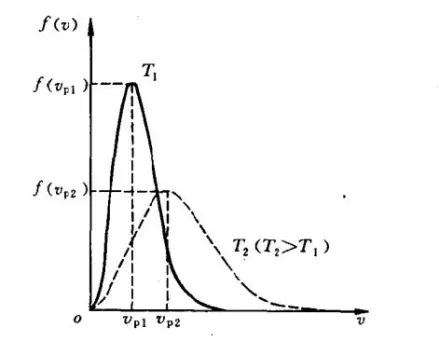
\includegraphics[width=0.5\textwidth]{image/Maxwell_speed_distribution.png}
\end{center}

从几何上理解了 \(4\pi v^2 dv\) 的来源后，函数 \(F(v) dv\) 的物理本质便一目了然：
\[
F(v) dv = \text{速度空间中半径为 }v\text{ 的球壳体积} \times \text{该速率处分子的概率密度}
\]
因此，\(F(v) dv\) 这个组合本身，就已经给出了一种最直接的统计意义——\textbf{它代表了速率落在 \(v\) 到 \(v+dv\) 这个微小区间内的分子，占全部分子总数的比例}。即：
\[
\frac{dN}{N} = F(v) dv
\]

现在我们把这个逻辑延伸到更一般的统计计算。在热力学与统计物理中，我们经常需要计算分子各种物理量的平均值，比如平均速率 \(\bar{v}\)、方均速率 \(\overline{v^2}\)。此时，\(v^n f(v) dv\) 这一组合的积分就显得尤为关键。为什么叫“博弈”的公式？因为 \(v^n f(v) dv\) 本身就在诠释物理量的微观贡献。
\begin{itemize}
    \item \textbf{“局部的权重”：} 对于一个单独的速率点 \(v\) 附近的微小区间 \(dv\)，由 \(F(v)dv = f(v)dv\) 我们知道，这部分分子出现的概率是 \(f(v)dv\)。如果我们想要计算这部分分子对某种速率幂 \(v^n\) 的贡献，那这一小群分子的贡献就是：
    \[
    v^n \times f(v)dv
    \]
    \item \textbf{“全局的积分”：} 既然在速率 \(v\) 处的贡献是 \(v^n f(v) dv\)，那么把所有可能的速率 \(v\) 都考虑进去（即积分），我们就得到了该速率幂的全局统计平均值：
    \[
    \overline{v^n} = \int_{0}^{\infty} v^n f(v) dv
    \]
\end{itemize}
\textbf{这里有一个极易踩坑的统计学概念需要注意：} 如果是求\textbf{全体分子}的全局平均值，上述积分公式 \textbf{\(\int_{0}^{\infty} v^n f(v) dv\)} 是正确的。由于速率必须大于等于0（全空间总概率为1，即 \(\int_{0}^{\infty} f(v) dv = 1\)），这个积分结果就直接代表了物理量 \(\langle v^n \rangle\)。然而，如果你面对的是\textbf{“截断”的区间}，比如题目询问“速率落在 \(v_1\) 到 \(v_2\) 之间的\textbf{这些分子}，其 \(v^n\) 的平均值是多少？”，此时你必须加上归一化条件：

\[
\overline{v^n}_{(v_1, v_2)} = \frac{\int_{v_1}^{v_2} v^n f(v) dv}{\int_{v_1}^{v_2} f(v) dv}
\]

\textbf{分母 \(\int_{v_1}^{v_2} f(v) dv\)} 代表的是速率在 \(v_1 \sim v_2\) 之间的分子\textbf{数量占总数的比例}。这个比例的存在，保证了我们在求算“该区间内分子的平均速率”时，分母是该区间的分子总数，而不是整个系统的总数。所以\textbf{ \(v^n f(v)dv\) 的含义}就是：
\begin{center}
    \textbf{“\(v^n f(v)dv\) 代表的是：速率在 \(v\) 附近极小范围 \(dv\) 内的所有分子，其物理量 \(v^n\) 对【全系统统计平均值】做出的微小贡献（已除以总分子数 \(N\) 归一化）。”}
\end{center}
当 \(n=1\) 时，\(\int v f(v) dv\) 得到平均速率 \(\bar{v}\)；当 \(n=2\) 时，\(\int v^2 f(v) dv\) 得到方均速率 \(\overline{v^2}\)，由此麦克斯韦速率分布的三个特征速率，就此得出，它们的核心物理意义和公式如下：

\begin{table}[H]
\centering
\caption{三个特征速率对比}
\begin{tabular}{>{\centering\arraybackslash}m{2.5cm} >{\centering\arraybackslash}m{2.5cm} >{\centering\arraybackslash}m{5cm} >{\arraybackslash}m{5cm}}
\toprule
\textbf{特征速率} & \textbf{符号} & \textbf{数学公式 (用 \(m\) 和 \(T\) 表示)} & \textbf{核心物理意义} \\
\midrule
最概然速率 & \(v_p\) & \(\sqrt{\frac{2kT}{m}}\) & 概率最大的速率。分布曲线峰值对应的速率，表示在该速率附近单位速率区间内的分子数占比最多。 \\
平均速率 & \(\bar{v}\) & \(\sqrt{\frac{8kT}{\pi m}}\) & 分子速率的算术平均值。在计算分子平均自由程等问题时常用到。 \\
方均根速率 & \(v_{rms}\) & \(\sqrt{\frac{3kT}{m}}\) & 速率平方平均值的平方根。由于分子的平均平动动能 \(\bar{\epsilon}_k = \frac{3}{2}kT\)，它常用于计算分子平均动能。 \\
\bottomrule
\end{tabular}
\end{table}


对于同一种气体在相同温度下，三个速率的大小关系为：
\[
v_p < \bar{v} < v_{rms}
\]
其比值为：
\[
v_p : \bar{v} : v_{rms} = \sqrt{3} : \sqrt{\frac{8}{\pi}} : \sqrt{3} 
\]

三个速率均与温度的平方根 (\(\sqrt{T}\)) 成正比，与分子质量的平方根 (\(1/\sqrt{m}\)) 成反比。



\subsection{气体分子动理论}

在气体分子运动论中，一个非常重要的量是\textbf{平均自由程}（mean free path），记作 \(\lambda\)。它表示一个分子在两次相互碰撞之间平均能够走过的路程。这个量把微观碰撞过程和宏观输运现象联系起来，在理解扩散、热传导和黏滞现象时都很重要。


我们先把气体分子近似看成直径为 \(d\) 的刚性小球。若只盯住其中某一个分子，并暂时把其他分子视为静止，那么当这个分子以速率 \(v\) 在时间 \(\Delta t\) 内前进时，它扫过的不是一条几何直线，而是一个半径为 \(d\) 的圆柱形碰撞区域，其体积为
\[
\Delta V=\pi d^2 v\Delta t.
\]
如果单位体积内的分子数密度为
\[
n=\frac{N}{V},
\]
那么在这段时间内，这个圆柱体中平均包含的分子数，也就是预期碰撞次数，为
\[
\Delta N=n\,\Delta V=n\pi d^2 v\Delta t.
\]
于是单位时间内的平均碰撞频率可写为
\[
\nu=\frac{\Delta N}{\Delta t}=n\pi d^2 v.
\]
若把两次碰撞之间的平均时间记为 \(\tau\)，则有
\[
\tau=\frac{1}{\nu}.
\]
因此平均自由程就是
\[
\lambda=v\tau=\frac{v}{\nu}=\frac{1}{n\pi d^2}.
\]

这个结果抓住了平均自由程的核心思想：\textbf{平均自由程等于每单位体积里的潜在碰撞对象数目与碰撞几何截面共同决定的尺度。}



不过上面的推导把其余分子都视为静止，这只是第一近似。真实气体中所有分子都在做热运动，因此真正决定碰撞频率的，是分子之间的\textbf{相对速率}而不是某一个分子的绝对速率。

对麦克斯韦分布作更精确处理后，可以证明平均相对速率会比单分子的平均速率多出一个 \(\sqrt{2}\) 的因子。因此平均自由程的标准结果应修正为
\[
\lambda=\frac{1}{\sqrt{2}\,n\pi d^2}.
\]
再用数密度 \(n=N/V\) 表示，可写成
\[
\lambda=\frac{V}{\sqrt{2}\,N\pi d^2}.
\]
再代入理想气体状态方程
\[
pV=nk_{\mathrm B}T,
\qquad
n=\frac{pV}{k_{\mathrm B}T},
\]
便得到常用形式
\[
\lambda=\frac{k_{\mathrm B}T}{\sqrt{2}\,\pi d^2 p}.
\]

从这个式子可以直接读出物理意义：压强越大，气体越稠密，碰撞越频繁，因此平均自由程越短；温度越高，在相同压强下数密度越低，因此平均自由程越长；分子有效直径越大，碰撞截面越大，因此平均自由程也越短。



如果定义碰撞截面
\[
\sigma=\pi d^2,
\]
那么平均自由程公式还可以写成更紧凑的形式：
\[
\lambda=\frac{1}{\sqrt{2}n\sigma}.
\]
这在统计物理中很常见，因为它把分子几何大小的信息都压缩进了 \(\sigma\) 这个量里。


\subsection{热力学}

热力学有一种很奇特的气质：它几乎不关心世界到底是由什么构成的，却仍然能说出极其可靠的话。你不必先知道分子怎样撞来撞去，也不必先知道原子怎样振动，只要承认系统有温度、体积、压强，有时候还能和外界交换热量、做一点功，那么一整套惊人的规律就已经在那里等着你了。它像是在告诉我们：自然界里有些事情，不依赖细节，也照样成立。

最先遇到的，是内能这个量。所谓内能，并不是某个神秘储存在物体里的“热的东西”，而只是系统内部所有微观运动和相互作用能量的总和。一个气体分子在乱跑，分子与分子之间在吸引、排斥，在振动、转动，这些都算在里面。于是当系统从一个状态变到另一个状态时，内能也会改变。热力学第一定律说的正是这件事：能量不会无缘无故冒出来，也不会无缘无故消失，它只能从一种形式转成另一种形式。
\[
\mathrm dU=\delta Q-\delta W.
\]
这里 \(\delta Q\) 表示外界传给系统的热量，\(\delta W\) 表示系统对外所做的功。这个式子看起来简单，但它包含着极深的判断：热和功都不是“系统自身携带的状态量”，它们是过程中的能量交换方式；只有 \(U\) 才是状态函数。也就是说，你不能问“这个系统有多少热”或者“这个系统有多少功”，就像你不能问“这个人有多少走路”一样。走路是过程，不是存货。热和功也是这样。

对最常见的准静态体积变化过程，系统对外做的机械功是
\[
\delta W=p\,\mathrm dV,
\]
于是第一定律常写成
\[
\mathrm dU=\delta Q-p\,\mathrm dV.
\]
这个式子有一种朴素的画面感：如果你给气体一点热量，这些能量一部分可能真的留在系统里，让分子运动更剧烈，也就是使内能增大；另一部分则可能被气体拿去推活塞，变成对外做功。热量并不自动等于温度升高，因为系统也许一边吸热，一边在“干活”。这正是初学热学时最容易忽略、但又最重要的事实。

例如在等体过程中，\(\mathrm dV=0\)，系统不做体积功，于是
\[
\delta Q=\mathrm dU.
\]
你给它多少热，内能就增加多少。而在等压膨胀中，系统一边吸热一边推动外界，热量就分成了两部分：一部分变成内能，一部分变成体积功。至于等温过程，若是理想气体，由于内能只与温度有关，温度不变便意味着
\[
\mathrm dU=0,
\]
所以吸收的热量全部都拿去做功：
\[
\delta Q=\delta W.
\]
这几种过程表面上只是不同的实验条件，实际上却像是在向你展示同一条能量守恒定律的不同侧面。

热力学真正变得迷人的地方，是当我们把这些过程首尾相接，构成一个\textbf{热循环}的时候。所谓循环，就是系统兜了一圈，又回到原来的状态。既然最终状态和初态相同，那么内能作为状态函数，变化必定为零：
\[
\Delta U=0.
\]
于是沿整个循环积分第一定律，就得到
\[
Q_{\mathrm{cycle}}=W_{\mathrm{cycle}}.
\]
也就是说，在一个完整循环里，系统净吸收的热量，必定等于系统净输出的功。这是热机一切讨论的基础。热机并不是凭空从某个地方“制造功”，它只是把从高温热源拿来的部分热量，转换成了机械功，剩下的则不得不丢给低温热源。

如果你把这个循环画在 \(p-V\) 图上，事情会变得更直观。循环围成的面积，就是系统在一个周期里对外做的净功：
\[
W=\oint p\,\mathrm dV.
\]
\textbf{顺时针循环，通常表示系统对外输出功；逆时针循环，则表示外界反过来对系统做功。}于是热机、冰箱、空调，看上去像三种完全不同的机器，其实都不过是在 \(p-V\) 图上选择不同方向绕圈罢了。热力学最动人的地方之一，就在这里：复杂的机器，最后都能被还原成几条曲线围出来的一块面积。

但紧接着，热力学告诉我们一个更深刻、也更不近人情的事实：并不是所有吸收的热量都能变成功。假设一台热机从高温热源吸热 \(Q_h\)，向低温热源放热 \(Q_c\)，并输出功 \(W\)，那么由能量守恒可知
\[
W=Q_h-Q_c.
\]
热效率定义为
\[
\eta=\frac{W}{Q_h}=1-\frac{Q_c}{Q_h}.
\]
如果你刚学到这里，也许会天真地想：那我只要把 \(Q_c\) 变成零，不就能把所有热量都变成功了吗？可惜自然界不答应。热力学第二定律说，热量自发地从高温流向低温，而不可能在不付出额外代价时反过来；因此任何工作在两个热源之间的热机，都不可能把吸收的热量全部转化为功。总得有一部分废热，被排到低温处去。

在所有可能的可逆热机中，卡诺热机给出了效率的上限：
\[
\eta_{\mathrm C}=1-\frac{T_c}{T_h}.
\]
这里 \(T_h\) 是高温热源温度，\(T_c\) 是低温热源温度。这个公式美得几乎让人不安，因为它完全不提工作物质是什么，也不提机器内部结构如何复杂。蒸汽机也好，燃气轮机也好，某种你从未见过的古怪热机也好，只要它们在这两个温度之间工作，效率上限都只能是这个数。仿佛自然界在背后冷冷地说：我不在乎你设计得多聪明，规矩就是规矩。

从这里你就能明白为什么低温热源如此重要。热机必须“把不要的东西丢掉”，就像你整理房间，不能只往一边堆而不留出口。没有冷源，热机就无处排放那部分无法转成功的热量；没有温差，也就没有持续做功的可能。我们平时说“利用热能”，其实真正利用的并不是某个绝对的高温，而是\textbf{温度差}。一切热机——从最早的蒸汽机到今天的发电站——都不过是在设法利用这个温差。

如果再把眼光放宽一点，热力学还告诉我们什么叫过程的方向性。力学方程往往允许时间反演：把速度反过来，电影倒着放，好像也还能成立。可是热学世界里却有明显的“前后之分”：热茶自己凉下去是常事，冷茶自己变热却从未见过；气体自己充满房间很自然，自己缩回角落却不发生。于是我们引入熵这个量，来刻画这种宏观过程的方向。对可逆过程，熵变满足
\[
\mathrm dS=\frac{\delta Q_{\mathrm{rev}}}{T},
\]
而对孤立系统，自发过程总满足
\[
\Delta S\ge 0.
\]
这并不是说世界总在“变乱”这么简单，而是说：系统总倾向于走向那些更容易实现、对应更多微观方式的状态。热力学第二定律真正深刻之处，不是禁止某件事“绝对不可能”，而是告诉你某些过程虽然在微观上未必被禁止，但在宏观上几乎永远不会发生。

于是，当我们回头看第一定律和热循环，就会发现热力学其实在同时讲两件事：第一定律告诉你“账目必须平”；第二定律告诉你“钱虽然平了，但花法并不对称”。能量守恒保证你不会无中生有，而熵增原则则规定哪些变化能自然发生，哪些变化必须借助外界安排。也正因为这两条规律一起存在，热学才既像会计学一样精确，又像哲学一样带有时间方向的意味。

如果你真正在脑海里留下一个热力学的图景，我希望不是一堆公式，而是一幅这样的画面：一个系统像机器一样运转，和外界交换热量，推活塞，走完一圈又回到原处；在这一圈里，内能可以起伏，但最终归零，热量和功彼此转换；然而不是所有热量都能变成功，因为世界偏爱从高温走向低温，偏爱从少数可能走向多数可能。热力学就是把这种“偏爱”写成定律的学问。

\subsection{热容}

如果再往前走一步，就会遇到一个很实际、也很像工程师会问的问题：同样给两个物体一点热量，为什么一个温度上升得很快，另一个却仿佛若无其事？一小勺水在酒精灯上很快就烫起来，而一大块铁即使同样吸收一些能量，也未必显得那么“激动”。于是我们引入热容这个量。热容并不是“物体能装多少热”，而是说：当你想把一个系统的温度升高一点时，究竟要付出多少热量。它定义为
\[
C=\frac{\delta Q}{\mathrm dT}.
\]
这个定义本身就提醒我们，热容和过程有关。因为 \(\delta Q\) 不是状态函数，所以你若不说明系统是在什么约束下升温，这个比值就不一定唯一。对气体尤其如此：你一边加热，一边允许它膨胀，系统就会顺手拿一部分能量去做功；而你若把它关在定容容器里，同样升高一度，所有热量几乎都只能老老实实地留在系统内部。

因此最重要的两个热容，是定容热容和定压热容。定容时 \(\mathrm dV=0\)，系统不做体积功，于是第一定律给出
\[
\delta Q=\mathrm dU,
\qquad
C_V=\left(\frac{\partial U}{\partial T}\right)_V.
\]
定压时系统一边吸热一边膨胀，于是有
\[
C_P=\left(\frac{\delta Q}{\mathrm dT}\right)_P.
\]
对于理想气体，把焓定义为
\[
H=U+pV,
\]
再结合第一定律与定压条件，可以得到
\[
C_P=\left(\frac{\partial H}{\partial T}\right)_P.
\]
这就是说，定容热容关心的是“把温度升高所需的内能变化”，而定压热容关心的则是“除了内能变化，还要替系统支付膨胀做功这笔账”。所以一般总有
\[
C_P>C_V.
\]
对理想气体更进一步，还能得到 Meyer 关系：
\[
C_P-C_V=nR.
\]
如果写成每摩尔的形式，就是
\[
C_{P,m}-C_{V,m}=R.
\]
这是一条很漂亮的关系，因为它说明定压比定容“多花掉”的那部分热量，恰好就对应每摩尔气体膨胀时所需的那一点点额外代价。而这就是摩尔热容。它定义为
\[
C_m=\frac{1}{n}\frac{\delta Q}{\mathrm dT},
\qquad
\delta Q=nC_m\,\mathrm dT.
\]
摩尔热容的好处在于，它更直接地把热学性质和微观自由度联系起来。对单原子理想气体，能量均分定理告诉我们，三个平动自由度每个贡献 \(\frac12 k_{\mathrm B}T\)，于是每个分子的平均内能是 \(\frac32 k_{\mathrm B}T\)，每摩尔便是
\[
U=\frac32 RT,
\]
从而
\[
C_{V,m}=\frac32 R,
\qquad
C_{P,m}=\frac52 R.
\]
如果是双原子分子，在常温下转动自由度也开始参与，摩尔热容便会变大；温度再高一些，振动自由度也被激发，热容又会继续上升。于是热容这个看上去很“工程”的量，背后其实藏着分子到底有多少种储存能量的办法。一个系统热容大，不是因为它神秘地“爱吃热”，而是因为它有更多自由度，可以把你给它的能量分散安放到更多地方去。

接下来就轮到比热。日常语言里人们常把热容和比热混着说，但它们其实不是一回事。热容是整个物体的性质，一杯水和一桶水当然不同；比热容则是把“物体有多少料”这件事除掉之后，留下单位质量材料本身的特征。质量比热容定义为
\[
c=\frac{1}{m}\frac{\delta Q}{\mathrm dT},
\qquad
\delta Q=mc\,\mathrm dT.
\]
因此，比热容回答的是这样一个问题：如果我拿 \(1\,\mathrm{kg}\) 这种材料来升高一度，需要多少热量？水的比热大，所以它擅长“吞下很多热却不怎么升温”；金属的比热通常较小，所以它们更容易热起来，也更容易冷下来。这就是为什么海洋能缓和气候，而金属勺子放进热汤里很快就烫手。

所以，热容、比热和摩尔热容这三个名字，讲的其实是同一件事，只是看问题的尺度不同。热容问的是“这整个系统升高一度要多少热”；比热容问的是“单位质量的材料升高一度要多少热”；摩尔热容问的是“每摩尔物质升高一度要多少热”。它们像是同一个问题在三个不同镜头下的样子：一个是整台机器，一个是每公斤材料，一个是每 \(6.02\times10^{23}\) 个粒子的集合。热学常常就是这样——换个尺度看，同一件事就会显出完全不同的味道。

\subsection{准静态的热力学过程}

不过，当我们真的开始“算一个过程”时，事情才刚刚开始。前面那些公式大多是在告诉你有哪些量，可一旦系统真的从一个状态走到另一个状态，你就会立刻发现：不是每条路都一样，也不是每个量都像内能那样老实。热力学里最重要的一个训练，也许就是学会把“状态”和“过程”分开来看。状态函数只看起点和终点，比如 \(U\)、\(H\)、\(S\)；而热量 \(Q\) 和功 \(W\) 却是沿着具体路径一点点积累出来的，路径一换，数值就可能全变了。也正因如此，我们才会如此在意所谓的\textbf{准静态过程}。

所谓准静态，并不是说过程真的静止不动，而是说它走得足够慢，慢到系统在每一个瞬间都几乎还能被看成处于平衡态。活塞不是“砰”地一下被推过去，而是一点一点地挪；气体内部的压强和温度来得及重新分布，于是每一时刻你都还能给它写一个明确的 \(p\)、\(V\)、\(T\)。这听上去像是在对现实世界吹毛求疵，可它有一个极大的好处：只有在准静态条件下，许多过程量才可以被写成我们熟悉、也最好算的微分形式。比如体积功就能写成
\[
\delta W=p\,\mathrm dV.
\]
如果过程非常剧烈，系统内部根本来不及建立统一的压强，那么这个式子就未必还能直接使用了。换句话说，准静态并不只是“变化很慢”这么一个温和的形容词，它其实是在替我们争取使用平衡态方程和积分计算的资格。

于是，热力学计算的基本方法论就变得很清楚了。拿到一个过程，第一步不是急着代公式，而是先问三个问题：系统是什么？约束是什么？过程路径是什么？系统若是理想气体，我们就知道有状态方程
\[
pV=nRT.
\]
约束若是定压、定容、定温或绝热，就意味着在这条路径上某个量保持不变。路径一旦确定，功就从
\[
W=\int p\,\mathrm dV
\]
去算，内能变化就从状态函数关系去算，而热量再由第一定律
\[
\Delta U=Q-W
\]
或者写成
\[
Q=\Delta U+W
\]
补出来。也就是说，热学题真正的计算顺序，往往不是“先求热，再求功”，而是先凭状态方程和过程条件把路径摸清，再求容易求的那一个，最后用第一定律把另一个补齐。

例如在定容过程中，体积根本不变，所以 \(\mathrm dV=0\)，体积功自然立刻消失：
\[
W=\int p\,\mathrm dV=0.
\]
于是第一定律直接塌缩成
\[
Q=\Delta U.
\]
对理想气体来说，内能只与温度有关，因此若温度从 \(T_1\) 变到 \(T_2\)，便有
\[
\Delta U=nC_V(T_2-T_1),
\qquad
Q=nC_V(T_2-T_1).
\]
这个过程最好算，也最适合用来理解“热量并不等于功”这件事：你给进去的热，全部都留在系统内部，变成了分子运动的增加。

定压过程稍微复杂一点，因为系统一边吸热，一边还可能把活塞顶出去。若压强保持为常量 \(p\)，那么功马上可以由几何面积给出：
\[
W=p(V_2-V_1).
\]
再利用理想气体状态方程把 \(p\Delta V\) 换成 \(nR\Delta T\)，便可写成
\[
W=nR(T_2-T_1).
\]
与此同时，内能变化仍然是
\[
\Delta U=nC_V(T_2-T_1),
\]
所以热量就成了
\[
Q=nC_P(T_2-T_1).
\]
你会发现，这里之所以是 \(C_P\) 而不是 \(C_V\)，正是因为定压加热时，系统不仅要“把自己加热”，还得额外拿出一点能量去推动外界。于是定压热容总比定容热容更大，这不是定义上的巧合，而是过程路径在替它们制造差别。

等温过程又是另一番景象。对理想气体来说，只要温度不变，内能就不变，于是
\[
\Delta U=0.
\]
第一定律立刻告诉我们
\[
Q=W.
\]
也就是说，你给系统多少热，它就一边膨胀，一边把这些热原封不动地转成对外做功。若过程还是准静态的，那么用状态方程中的 \(p=nRT/V\) 代入功的积分，便得
\[
W=\int_{V_1}^{V_2}p\,\mathrm dV
=nRT\int_{V_1}^{V_2}\frac{\mathrm dV}{V}
=nRT\ln\frac{V_2}{V_1}.
\]
于是热量也同样是
\[
Q=nRT\ln\frac{V_2}{V_1}.
\]
这个对数常让初学者有点不舒服，但它其实只是因为压强在过程中不停变化，面积不再是简单的长方形，而是一条曲线下面积。

再看绝热过程。所谓绝热，并不是“温度不变”，而是系统与外界之间没有热交换：
\[
Q=0.
\]
因此第一定律变成
\[
\Delta U=-W.
\]
也就是说，系统若对外做功，就只能消耗自己的内能，所以温度会下降；反过来，若外界压缩系统并对它做功，它的温度就会上升。对于理想气体的准静态绝热过程，还能进一步导出泊松关系
\[
pV^{\gamma}=\text{常量},
\qquad
TV^{\gamma-1}=\text{常量},
\]
其中
\[
\gamma=\frac{C_P}{C_V}.
\]
一旦你记住这两个关系，绝热题的计算其实就有了固定套路：先用绝热关系把末态量联系起来，再由
\[
\Delta U=nC_V(T_2-T_1)
\]
求出内能变化，最后因为 \(Q=0\)，便知道
\[
W=-\Delta U.
\]
很多看上去花哨的活塞压缩和喷管膨胀问题，本质上都只是在这里面换了件衣服。

有时题目并不会老老实实告诉你“这是定压”或者“这是绝热”，它只会给你一条路径关系，比如
\[
pV^n=\text{常量}.
\]
这叫多方过程。别被名字吓到，方法其实仍然一样：先由路径关系把 \(p\) 写成 \(V\) 的函数，再代回
\[
W=\int p\,\mathrm dV
\]
求功；若系统还是理想气体，再用温度变化求 \(\Delta U\)，最后由第一定律求 \(Q\)。热力学里的很多题，表面不同，骨架却总是这一套：\textbf{先定路径，再算功；再用状态函数求内能；最后用第一定律闭合全局。}

从这个角度看，所谓“不同热力学过程的计算方法”，并不是要你死记一堆彼此孤立的公式，而是要你学会认出每一条公式背后对应的物理约束。定容对应“做不了体积功”，定压对应“边加热边顶开外界”，等温对应“热全变成功”，绝热对应“功只能拿内能来付账”。一旦这些图像在脑中站稳，公式不过是它们的速记符号。热力学真正高明的地方，正在这里：它从不直接替你算完一切，它只是把你领到一套极其可靠的账本面前，然后让你按着自然界的规矩，把每一笔能量都对清楚。

如果想把刚才那几个基本过程放在一起比一比，最直观的办法就是列一张小表。定容时功为零，热全归内能；定压时功与热都跟温度变化成正比，但热容更大；等温时内能不动，热与功一一对消；绝热时热为零，系统只能拿内能的变化去垫付功。这张表就像一张速查卡，把每个过程最硬的骨头都摆在眼前了。

\begin{center}
\begin{tabular}{|c|c|c|c|}
\hline
\textbf{过程} & \textbf{内能变化 $\Delta U$} & \textbf{热量 $Q$} & \textbf{功 $W$} \\
\hline
\textbf{定容} & $nC_V\Delta T$ & $nC_V\Delta T$ & $0$ \\
\hline
\textbf{定压} & $nC_V\Delta T$ & $nC_P\Delta T$ & $p\Delta V = nR\Delta T$ \\
\hline
\textbf{等温} & $0$ & $nRT\ln\frac{V_2}{V_1}$ & $nRT\ln\frac{V_2}{V_1}$ \\
\hline
\textbf{绝热} & $nC_V\Delta T$ & $0$ & $-nC_V\Delta T$ \\
\hline
\end{tabular}
\end{center}

\subsection{卡诺循环和熵}

不过，这些过程在热力学里很少被单独拿出来欣赏，它们更像一些基本的乐高积木，真正的建筑是那些把它们首尾衔接成的\textbf{热力学循环}。循环的定义并不神秘：系统从某个状态出发，走过一串过程，最后又回到出发点。因为终点就是起点，所有状态函数——内能 $U$、焓 $H$、熵 $S$——在走完一圈后的净变化都只能是零：
\[
\Delta U = 0,\quad \Delta H = 0,\quad \Delta S = 0.
\]
但功和热就不一样了，它们不是状态函数，完全可以一路上进进出出，只要最后总的账目是平的就行。把第一定律沿整个循环积分一次，就得到
\[
\oint \delta Q = \oint \delta W,
\quad\text{或简写为}\quad Q_{\text{net}} = W_{\text{net}}.
\]
换句话说，循环从外界净吸收了多少热量，就净对外输出了多少机械功。这句话听起来像是同义反复，可它恰恰是所有热机、制冷机和热泵最底层的能量记账本。这有一个简单快速的判断方法\textbf{顺时针做正功，放热；逆时针循环做负功，吸热。}这原因也很简单，因为循环一圈内能变化量为0，所以$W=Q$，而顺时针对于上面的曲线体积增大，对外做正功，与下面的曲线做的负功做差后留下的面积就是做一圈的总功了。

在所有可能的热力学循环里，有一个循环的地位几乎像神灵一样，那就是卡诺循环。它不是蒸汽机，也不是内燃机，而是一个理想化的思想模型——由两个等温过程和两个绝热过程交替组成。如果你把这个循环画在一张 $pV$ 图上，它就像一只被压扁了的矩形，只不过上下底是水平的等温线，左右边是陡峭的绝热线。

\begin{center}
    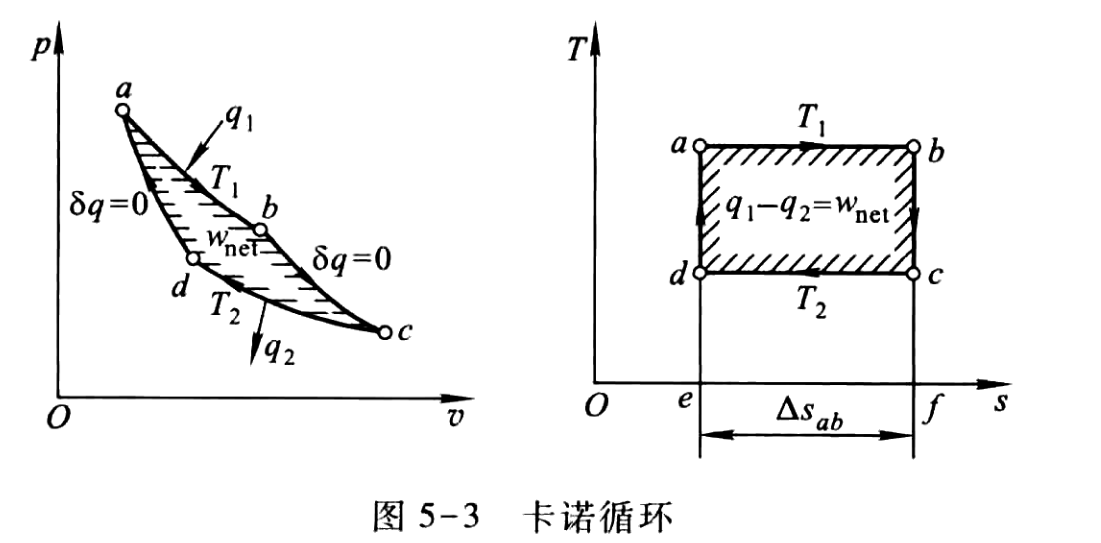
\includegraphics[width=0.7\textwidth]{image/kanuoxunhuan.png}
\end{center}

循环可以这样走：第一步，让系统在高温 $T_h$ 下等温膨胀，从高温热源吸热 $Q_h$，对外做正功，内能纹丝不动；第二步，让它绝热膨胀，温度从 $T_h$ 掉到 $T_c$，继续对外做功，但靠的是消耗自身内能；第三步，在低温 $T_c$ 下等温压缩，外界对系统做功，系统向低温热源放热 $Q_c$；第四步，绝热压缩，温度从 $T_c$ 回升到 $T_h$，外界继续对系统做功，把内能压回来。四步走完，机器回到起点，干干净净地走完一圈。

把这个循环的热量账本摊开：高温吸进 $Q_h$，低温排出 $Q_c$，净得的热量 $Q_h - Q_c$ 全部变成了对外做的净功 $W$。于是热机效率就是
\[
\eta = \frac{W}{Q_h} = 1 - \frac{Q_c}{Q_h}.
\]

卡诺循环真正深刻的地方，不是这个公式本身，而是它揭示的一个事实：\textbf{效率只取决于两个热源的温度，完全不依赖于用什么工质，也不依赖于机器的内部结构。} 对理想气体可以推导，对任意物质也可以推导；用蒸汽可以，用空气可以，甚至用某种你从未想象过的古怪液体，只要循环是可逆的，结果都一样：
\[
\eta_{\text{Carnot}} = 1 - \frac{T_c}{T_h}.
\]
这里 $T_h$ 和 $T_c$ 用的是热力学温标，也就是开尔文温度。这个公式像是自然界的定价标签：高温热源愿意给你多少热量，低温热源不得不接收多少废热，两者之间的温差决定了你能把那部分热量转换成有用功的比例上限。

如果你沿着这个思路再往前走一步，就会发现卡诺循环还藏着一件更贵重的东西。把效率公式改写一下：
\[
1 - \frac{Q_c}{Q_h} = 1 - \frac{T_c}{T_h}
\quad\Longrightarrow\quad
\frac{Q_h}{T_h} = \frac{Q_c}{T_c}.
\]
这个等式看上去只是移项整理的结果，但它意味着：在可逆循环中，系统从高温热源吸收的热量与温度之比，恰好等于它向低温热源放出的热量与温度之比。如果把 $Q/T$ 这个量看作某种“热量温度比重”，那么在一个可逆循环里，这个比重的收支竟然是平衡的。

这还不是全部。再进一步，如果我们把这个循环切碎，变成无数个无穷小的卡诺循环叠在一起，对每一个微小循环，都有
\[
\frac{\delta Q_h}{T_h} = \frac{\delta Q_c}{T_c}.
\]
当我们把所有这些微小循环拼成一个任意的可逆循环时，热量的出入便不再是两个热源，而是一路上无数个不同温度的微小热交换。但不论这条路多么曲折，总有一个量会始终保持均衡：
\[
\oint \frac{\delta Q_{\text{rev}}}{T} = 0.
\]
这个积分等于零，意味着什么？意味着被积函数 $\delta Q_{\text{rev}}/T$ 的积分与路径无关，只取决于起点和终点。这正是状态函数的标志性特征。于是克劳修斯站了出来，定义了一个新的状态函数——\textbf{熵}：
\[
\mathrm dS = \frac{\delta Q_{\text{rev}}}{T}.
\]
对于从一个状态到另一个状态的有限变化，熵变就是
\[
\Delta S = \int_{i}^{f} \frac{\delta Q_{\text{rev}}}{T}.
\]
注意那个下标“rev”绝不是摆设。它提醒你，这个定义里的热量是在可逆过程中传递的。熵本身是状态函数，它的变化只取决于初态和末态，但你计算它的时候，需要找一条可逆路径来搭桥——即使真实过程完全不可逆，你也得构造一条可逆的假想路径去算 $\Delta S$。

熵被定义出来之后，热力学第二定律终于有了一个精确的数学表述：对孤立系统（或者系统加环境一起考虑），任何自发过程都满足
\[
\Delta S \ge 0.
\]
等号对应可逆过程，大于号对应不可逆过程。这意味着，孤立系统的熵永远不会自己减少。热量从高温流向低温，气体自由膨胀，墨水滴进清水——所有这些过程之所以自发发生，不是因为它们被什么神秘力量驱使，而是因为它们的总熵在增加。反过来，想让熵减少，比如把热量从低温抽回高温，让气体自己缩回角落，你非得从外界输入功不可，而这个过程本身又会引起周围环境的熵增，最终总的 $\Delta S$ 仍然非负。

但这里有一个耐人寻味的问题：$\Delta S = \int \delta Q_{\text{rev}}/T$ 这个定义，从头到尾都没有解释“为什么熵会自动增加”。它只是告诉我们怎么算，却没有告诉我们熵究竟是什么。你可能会觉得，一个被定义为 $\delta Q_{\text{rev}}/T$ 的积分竟然永远不会减少，这件事多少有点像是从天上掉下来的——它正确，但并不直观。

这时候，统计物理站了出来，用一种完全不同的语言重新讲述了熵的故事。它的出发点不再是热量和温度，而是\textbf{微观状态数}。

设想你有一个气体系统，里面有 $N$ 个分子，每个分子都在某个位置以某个速度运动。如果我们把每个分子的位置和速度都精确地记下来，这就构成了系统的一个\textbf{微观状态}。但实际做实验时，你根本不会关心每个分子在哪——你只关心压强、体积、温度这些宏观量。反过来看，一个给定的宏观状态（比如 $p=1\text{atm}, V=1\text{L}, T=300\text{K}$），其实对应着天文数字般多的微观状态：分子可以稍微挪一挪位置，稍微改一改速度，只要整体统计上还给出同样的压强和温度就行。

话说到这里，$\Delta S \ge 0$ 这个第二定律就不再是一个从天而降的禁令了，它变成了一句几乎像废话一样自然的话：孤立系统总是倾向于走向那些实现方式更多的状态。气体自由膨胀后，分子可摆放的位置大大增加，$\Omega$ 暴涨，熵自然增大；热茶凉下来，能量从集中分布变成弥散分布，微观状态数同样激增。反过来，要让熵减少，就等于要系统自发地从“很多种方式”跳到“很少几种方式”——这在概率上几乎不可能。不是绝对不可能，而是“几乎永远不会发生”。这就是第二定律的统计本质：它不是一条绝对的金规铁律，而是一条关于概率的、近乎确定性的陈述。

于是我们手里就有了两个熵：一个是克劳修斯熵，由热量和温度定义，擅长描述宏观过程中的能量流动方向；另一个是玻尔兹曼熵，由微观状态数定义，擅长解释“为什么会这样”。问题是，它们说的是同一个熵吗？换句话说，当我们用克劳修斯熵算出一个 $\Delta S$ 时，玻尔兹曼熵会给出同样的答案吗？

答案是肯定的，而且这个统一正是统计力学最精彩的成就之一。要看出这一点，我们先从玻尔兹曼熵出发，考虑一个系统在温度 $T$ 下与外界有微小的能量交换。系统吸收一小部分热量 $\delta Q$ 时，它的内能会增加 $\mathrm dU$，同时微观状态数 $\Omega$ 也会变化。

为了把玻尔兹曼描述和宏观量联系起来，我们考虑两个系统接触并交换能量，但整体与外界隔绝，总能量 $E_1+E_2 = E_{\text{total}}$ 守恒。孤立系统最终会自发走向平衡态。在统计物理的语言里，平衡态不是谁下了命令，而是总微观状态数最大的那个宏观态——因为系统在演化中，总是以压倒性的概率落在那些实现方式最多的状态上。

总微观状态数是两个系统各自状态数的乘积：
\[
\Omega_{\text{total}}(E_1,E_2) = \Omega_1(E_1)\,\Omega_2(E_2)。
\]
我们的目标是，在约束 $E_1+E_2 = E_{\text{total}}$ 下，找到使这个乘积最大的 $E_1$。直接处理乘积并不方便——它通常是天文数字的连乘，求导会很麻烦。但这里有一个简单却关键的数学技巧：对数函数是严格单调递增的，所以一个函数和它的对数在完全相同的位置取得最大值。把乘积取对数，乘积就变成了求和：
\[
\ln\Omega_{\text{total}} = \ln\Omega_1(E_1) + \ln\Omega_2(E_2)。
\]
这不仅让求导变得极其简单，也恰好给出了熵的可加性。乘以玻尔兹曼常数，总熵就是
\[
S_{\text{total}}(E_1,E_2) = k_{\text{B}}\ln\Omega_1(E_1) + k_{\text{B}}\ln\Omega_2(E_2)。
\]
因此，最大化总微观状态数，完全等价于最大化总熵。接下来，只需要用微积分找到总熵极大的位置就可以了。

用约束条件消去 $E_2 = E_{\text{total}}-E_1$，总熵变成 $E_1$ 的一元函数：
\[
S_{\text{total}}(E_1) = k_{\text{B}}\ln\Omega_1(E_1) + k_{\text{B}}\ln\Omega_2(E_{\text{total}}-E_1)。
\]

平衡态对应总熵极大。对 $E_1$ 求导并令其为零：
\[
\frac{\mathrm dS_{\text{total}}}{\mathrm dE_1} = 0。
\]
第一项直接求导，第二项应用链式法则（$\mathrm dE_2/\mathrm dE_1 = -1$），得到
\[
\frac{\mathrm dS_1}{\mathrm dE_1} - \frac{\mathrm dS_2}{\mathrm dE_2} = 0，
\]
即
\[
\frac{\mathrm dS_1}{\mathrm dE_1} = \frac{\mathrm dS_2}{\mathrm dE_2}。
\]

也就是说，热平衡时，两个系统的**熵对能量的变化率**必然相等。这是一个不依赖于任何宏观经验、纯粹从统计计数中推导出来的共同强度量。我们把它记为
\[
\frac{1}{T} \equiv \frac{\mathrm dS}{\mathrm dE}。
\]
为什么叫它温度的倒数？因为从能量流动方向看，$\mathrm dS/\mathrm dE$ 较小的系统更愿意给出能量，较大的系统更愿意接收能量——这和日常经验中“热量从高温流向低温”恰好相反。给它加上倒数，就得到了我们熟悉的温度：$\mathrm dS/\mathrm dE$ 大，对应温度低；$\mathrm dS/\mathrm dE$ 小，对应温度高。再用理想气体做个具体计算，这个定义给出的 $T$ 与开尔文温标完美吻合。至此，温度不再是独立的基本概念，而是从熵与能量的微观关系中长出来的量。

在这个定义下，对一个微小的可逆热量交换过程，能量变化 $\mathrm dE$ 刚好等于吸收的热量 $\delta Q$（不做体积功时），于是自然得到
\[
\mathrm dS = \frac{1}{T}\,\mathrm dE = \frac{\delta Q}{T}。
\]
克劳修斯熵的微分形式，就这样从玻尔兹曼熵和温度的统计定义中推导了出来。两条路线在此合拢，不再需要额外的假设。

现在，假如能量的变化仅仅来自热量交换（不做体积功），那么 $\mathrm dE = \delta Q$。于是
\[
\mathrm dS = \frac{\delta Q}{T}.
\]
这就是克劳修斯熵的微分形式。如果在可逆路径上积分，就正好回到 $\Delta S = \int \delta Q_{\text{rev}}/T$。

这样一来，两条熵的定义就在可逆过程中完美地统一了：玻尔兹曼熵从微观计数出发，推演出了克劳修斯熵的表达式；反过来，克劳修斯熵的计算结果，也就等于 $\Delta S = k_{\text{B}}\Delta(\ln\Omega)$。前者告诉你“怎么算”，后者告诉你“本质是什么”。你可以把克劳修斯熵看作宏观世界的操作手册，玻尔兹曼熵则是在微观世界里的那幅底片——两者拍的是同一张照片，只不过镜头不同。

更重要的是，这个统一关系还解释了一个常常令人困惑的现象：当不可逆过程发生时，用克劳修斯熵公式时你不能直接把真实过程的 $\delta Q/T$ 积分，因为真实过程中系统可能并不处于平衡态，温度本身就没有统一定义。但你可以构造一条连接初态和末态的可逆路径，算出 $\Delta S$，而玻尔兹曼熵 $\Delta S = k_{\text{B}}\ln(\Omega_f/\Omega_i)$ 则直接告诉你，这个值对应的是微观状态数增加了多少倍。不可逆过程的熵增，本质上就是系统从一种实现方式较少的状态，自发演化到了实现方式多得多的状态。

所以，两个熵的关系可以用一个简单的话收束：\textbf{克劳修斯熵是宏观的热力学路径积分，玻尔兹曼熵是微观的排列组合计数；在同一条可逆路径上，它们说的完全是同一件事；而在不可逆的真实世界里，玻尔兹曼熵告诉我们为什么熵一定增加——因为概率站在更多微观状态数的那一边。} 热力学第二定律也因此不再像一个暴君式的命令，而更像一句温和但几乎无法反驳的陈述：世界倾向于走向那些更容易发生的事。


\newpage
\section{经典波动学基础}

在钻进量子力学的迷宫之前，我们得先把一件更简单的事彻底搞清楚——波。不是量子波，是普通的波。水面上丢一颗石子，声带振动一下，吉他弦拨一下——这些东西看起来完全不一样，但它们背地里用的是一套相同的数学把戏。

这一节我们只待在一个地方：经典世界。没有概率幅，没有不确定性原理，只有实实在在的、你能用耳朵听到的波。



\subsection{简谐运动——点的运动学方程}

在自然界与工程实践中，广泛存在一类振动现象：物体在某个平衡位置附近做周期性往复运动。例如轻质弹簧一端固定，另一端连接一个可以忽略摩擦的质点，当质点偏离平衡位置后释放，它将左右运动。进一步观察发现，质点所受的合力总是指向平衡位置，且合力的大小与质点偏离平衡位置的位移大小成正比。这种运动形式称为\textbf{简谐运动}。

设质点的平衡位置为坐标原点 \(O\)，在某一时刻 \(t\)，质点的位置坐标为 \(x\)（即偏离平衡位置的位移）。根据胡克定律与牛顿第二定律，质点所受的回复力 \(F\) 满足
\[
F = -kx,
\]
其中 \(k\) 为弹簧的劲度系数（正常数），负号表示力的方向与位移方向相反，始终指向平衡位置。由牛顿第二定律 \(F = ma\)，并注意到加速度 \(a = \ddot{x}\)，整理得简谐运动的动力学微分方程
\[
\ddot{x} + \frac{k}{m} x = 0.
\]
令 \(\omega^2 = \frac{k}{m}\)（\(\omega>0\) 为系统的固有角频率），则方程化为标准形式
\[
\ddot{x} + \omega^2 x = 0. \tag{1}
\]

学过微积分的我们都知道，方程 (1) 的通解可写为
\[
x(t) = C_1 \cos(\omega t) + C_2 \sin(\omega t),
\]
其中 \(C_1, C_2\) 为积分常数，由初始条件（初始位移与初始速度）确定。为了更直观地揭示振动的特征，通常将上式改写成振幅与初相的形式。设
\[
A = \sqrt{C_1^2 + C_2^2}, \quad \cos\varphi = \frac{C_1}{A}, \quad \sin\varphi = -\frac{C_2}{A},
\]
则可得简谐运动点的运动学方程
\[
\boxed{x(t) = A \cos(\omega t + \varphi)}. \tag{2}
\]
其中，\(A\) 表示最大位移，称为振幅；\(\omega\) 称为角频率；\(\varphi\) 称为初相位，它决定了初始时刻质点的运动状态；\(\omega t + \varphi\) 是相位，反映了质点振动的进程。表达式 (2) 清楚地表明：简谐运动中，质点的位移随时间按余弦（或正弦）函数规律变化，这是一种最简单的周期性运动。通过求导，还可以进一步得到速度和加速度的运动学方程：
\[
v(t) = \dot{x}(t) = -\omega A \sin(\omega t + \varphi), \quad a(t) = \ddot{x}(t) = -\omega^2 A \cos(\omega t + \varphi) = -\omega^2 x(t).
\]
最后这个关系再次验证了动力学方程 (1) 中加速度与位移成正比且方向相反的特性。

\subsection{波在空间传播——平面简谐波的波函数}

在上一小节我们已经完整得到了点的简谐运动，这样做简谐运动的点在介质里产生连续的波，波的每一个点都是在做简谐运动，那么我们如何从一个波源的运动学方程得到整个空间波的运动学方程呢？

考虑一维空间中一个\textbf{位于$x_0$的波源处做简谐运动的波源}产生的一个往右跑的正弦波：
\[
y(x,t) = A\cos(\omega (t-\frac{x-x_0}{u}) + \varphi).
\]
这个方程简单的描述了空间带来的相位，也就是当$t=0$时候波源开始震动时候，波传播到$x=x_p$需要的时间为$(x_p-x_0)/u$，也就是说对于P点，$t=(x_p-x_0)/u$才是它的“$t=0$”。为了简便方程，我们记$\omega/u=2\pi/\Lambda=k$，因而就引出了波数这个量告诉你波有多密），因而原方程可以简化为：
\[
y(x,t) = A\cos(k(x-x_0) - \omega t + \varphi).
\]
这个\textbf{方程完整描述了时空中任意一点$(x,t)$的位移}。

这里我要教你一个偷懒的技巧，后面会反复用到。写：
\[
\tilde{y}(x,t) = A e^{i(k - \omega t + \varphi)}.
\]
因为一维空间具有平移对称性，所以这里我们使用$x=x_0$来描述这个规律。对于我们写出的这个方程，真正的$y$是这个复数的实部。为什么要这么干？因为指数函数比余弦好算一万倍。两个波叠加的时候，你只需要把它们的复振幅加起来，最后再取实部——干净利落，不会漏掉因子2，不会搞错符号。你就把它当成一个记账工具，用完就取实部，不会出错。

我们现在就来使用这个小技巧来简要验证一个波动力学中的恒等式，我们考虑方向相同但频率稍有不同的两列波。要解决这个问题，我们要先回到波本身。定义相位$\theta = kx - \omega t$。如果你盯着波上的一个固定点（比如某个波峰），这个点的相位必须保持不变。$d\theta = k dx - \omega dt = 0$，所以：
\[
v_p = \frac{dx}{dt} = \frac{\omega}{k}.
\]
这叫相速度——波峰跑的速度。但这里藏着一个陷阱。如果$\omega/k$依赖于$k$（即不同频率的波跑得不一样快），那么一个有限的波包——比如你突然抖一下产生的脉冲——就会在前进中散开。这叫色散。深水波、光在玻璃里、弹性杆的弯曲波，都有色散。

那么波包整体移动的速度是多少？它不是波峰的速度，而是波包“信封”的速度。取两列频率和波数都差一点的波叠加：
\[
\tilde{y} = A e^{i(k_1 x-\omega_1 t)} + A e^{i(k_2 x-\omega_2 t)} = A e^{i(\bar{k}x-\bar{\omega}t)}\left(e^{i(\frac{\Delta k}{2}x-\frac{\Delta\omega}{2}t)} + e^{-i(\frac{\Delta k}{2}x-\frac{\Delta\omega}{2}t)}\right).
\]
括号里是$2\cos\left(\frac{\Delta k}{2}x - \frac{\Delta\omega}{2}t\right)$，所以：
\[
\tilde{y} = 2A Re(e^{i(\bar{k}x-\bar{\omega}t)}) \cos\left(\frac{\Delta k}{2}x - \frac{\Delta\omega}{2}t\right)= 2A\cos\left(\frac{\Delta k}{2}x - \frac{\Delta\omega}{2}t\right)\cos(\bar{k}x-\bar{\omega}t).
\]


\begin{wrapfigure}{L}{0.32\textwidth}
  \begin{center}
    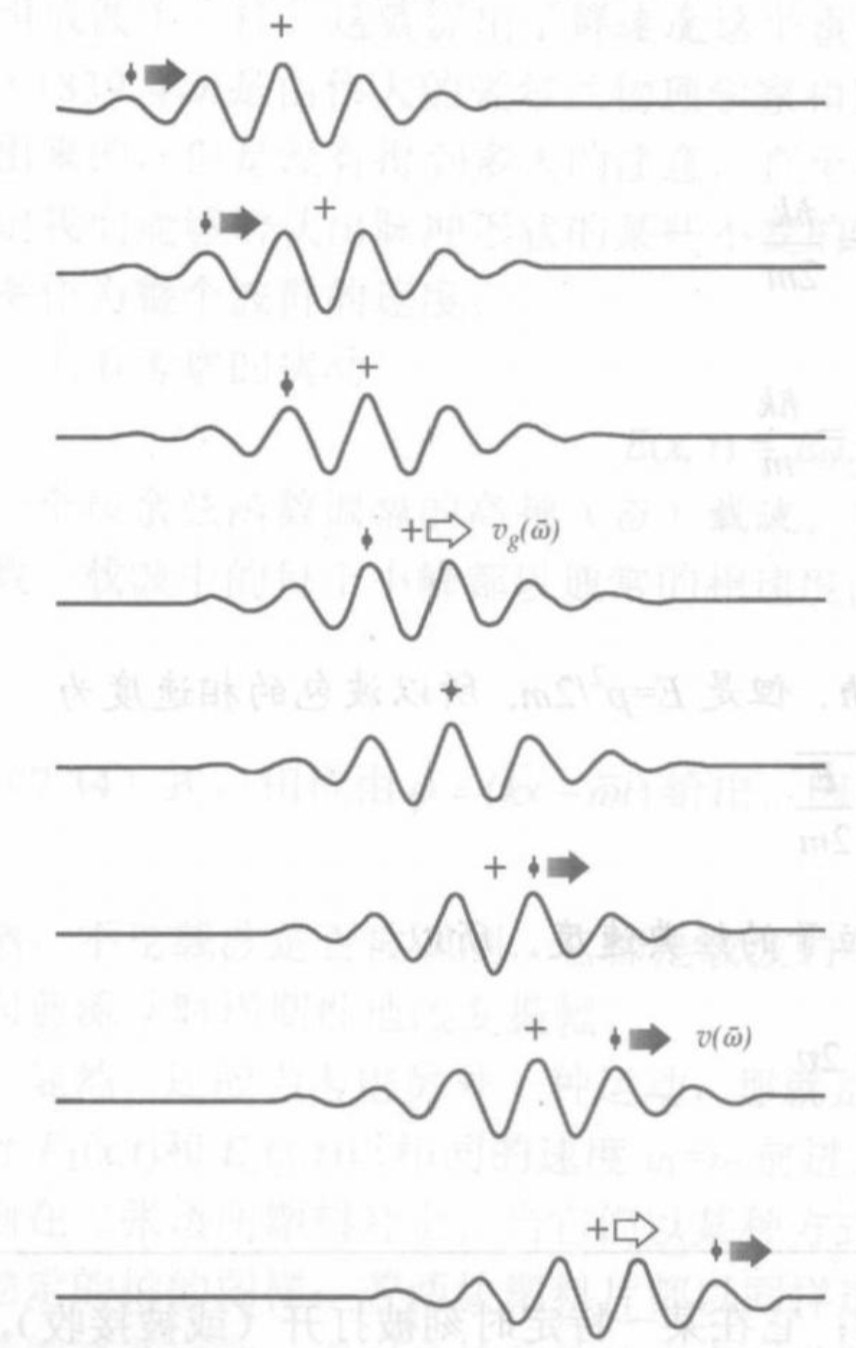
\includegraphics[width=0.3\textwidth]{image/qunv.png}
  \end{center}
    \caption{一个群的波包不断移动}
    \label{fig:qunv}
    \vspace{10pt}
\end{wrapfigure}

看到没有？一个快速振荡的载波（相速度$v_p=\bar{\omega}/\bar{k}$），外面套着一个慢变的包络。包络移动的速度就是群速度：
\[
v_g = \frac{\Delta\omega}{\Delta k} \to \frac{d\omega}{dk}.
\]
关键在这里：相速度只是波峰跑的速度，但波峰可以凭空消失在波包前面，又凭空从后面长出来——它不携带能量。只有群速度才告诉你“信号到底什么时候到”。你敲一根长杆，听到的“咚”的那一下，是以群速度跑的。相速度？那是数学游戏。

结果你看到了：一个慢变的包络骑在一个快变的载波上。当频率差足够大时，你能直接“听见”这个包络——那就是拍音。两个音叉频率差几赫兹，你听到的不是两个独立的声音，而是一个音量忽大忽小的声音，那个“呜—呜—呜”的频率就是频率差。这是音乐调音师耳朵里的物理学。



讨论完运动学方程，接下来我们就来看看它的“能量本征态”吧。波不只是形状在跑，它还把能量从一个地方搬到另一个地方。海浪能冲垮防波堤，声波能震碎酒杯——这不是开玩笑。

取绳子上的一小段$dx$，质量$\mu dx$（$\mu$是线密度），振动速度$\partial y/\partial t$，动能：
\[
dK = \frac12 \mu \left(\frac{\partial y}{\partial t}\right)^2 dx.
\]
势能从哪来？绳子弯曲的时候，它比平直的时候稍微长了一点，张力对这小段做了功。算出来：
\[
dU = \frac12 T \left(\frac{\partial y}{\partial x}\right)^2 dx.
\]
总能量密度：
\[
\mathcal{E}(x,t) = \frac12 \mu \left(\frac{\partial y}{\partial t}\right)^2 + \frac12 T \left(\frac{\partial y}{\partial x}\right)^2.
\]

对于简谐波$y=A\cos(kx-\omega t)$，代入波动方程$\mu\omega^2 = T k^2$，你会发现一个有意思的事：一个周期内，平均动能恰好等于平均势能。所以：
\[
\langle \mathcal{E} \rangle = \frac12 \mu \omega^2 A^2.
\]
能量以速度$v$传播，平均功率：
\[
\langle P \rangle = \langle \mathcal{E} \rangle v = \frac12 \mu \omega^2 A^2 v.
\]
公式很简单：频率越高、振幅越大、绳子越重，输送的能量就越多。

\subsection{叠加——波不打架}

因为波动方程是线性的，所以两列波可以在同一条绳子上共存，然后毫发无损地穿过去。总位移就是各自位移的代数和。就这么简单。但这个简单的原理，能衍生出一大堆有意思的现象。我们来看三种情况。

首先是最常见的情况：两列同频率、同方向的波。比如：
\[
\tilde{y}_1 = A_1 e^{i(kx-\omega t)},\quad \tilde{y}_2 = A_2 e^{i(kx-\omega t + \delta)}.
\]
加起来：
\[
\tilde{y} = (A_1 + A_2 e^{i\delta}) e^{i(kx-\omega t)}.
\]
合振幅的平方：
\[
A^2 = |A_1 + A_2 e^{i\delta}|^2 = A_1^2 + A_2^2 + 2A_1A_2\cos\delta.
\]

\begin{wrapfigure}{L}{0.32\textwidth}
  \begin{center}
    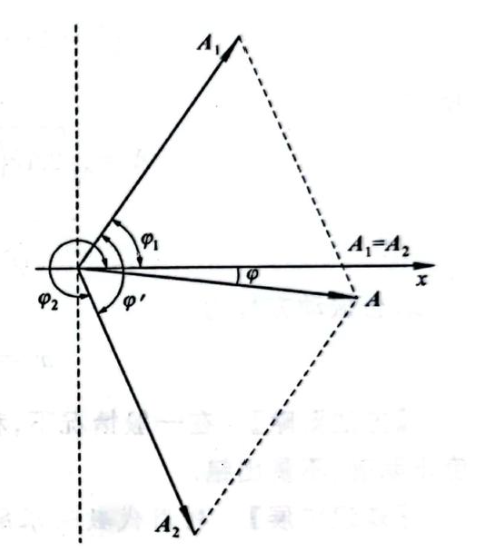
\includegraphics[width=0.3\textwidth]{image/rotvec1.png}
  \end{center}
    \caption{旋转矢量法看波合成}
    \label{fig:rotvec1}
    \vspace{10pt}
\end{wrapfigure}

这个结论也可以使用旋转矢量法更直观的得到，自然常数的技巧本质上是描述复平面上的旋转，因而我们只要绘制一个圆，对于角频率一样的两个波，它们的相位差总是不变，所以两个由振幅构成的矢量所合成的矢量也总是不变的，如图\ref{fig:rotvec1}，我们可以直观的看到这个平行四边形法则。

当$\delta=0$时，$A=A_1+A_2$——这叫相长干涉，波峰对波峰，变得更猛。当$\delta=\pi$时，$A=|A_1-A_2|$——这叫相消干涉，一个波峰撞上另一个波谷，可能完全抵消。能量去哪了？没消失，只是被重新分配到别的地方去了。这就是杨氏双缝实验的原理：光从两个缝出来，走到屏幕上某一点的路程差不同，相位差不同，有的地方亮，有的地方暗。如果光是粒子，不会出现暗纹。只有波，才会因为相位抵消而变暗。你看，这不就是波最迷人的地方吗？说它是幽灵也好，说它是数学游戏也罢，反正光就是这么干的——两个振动一碰头，既可能翻倍，也可能归零。







\bigskip

现在我们来看看一点不一样的情况，两列波频率依然相同，只不过一个波推着它上下振动（$X$方向），另一个波推着它左右振动（$Y$方向）我们盯着空间中的某个固定点。：
\[
X(t) = A_x \cos(\omega t + \varphi_x),\qquad Y(t) = A_y \cos(\omega t + \varphi_y).
\]
这两个振动频率相同，所以它们之间只有相对相位 $\delta = \varphi_y - \varphi_x$ 是重要的。我们想知道点 $(X(t),Y(t))$ 在平面上画出什么轨迹。

有没有办法把这两个实函数打包成一个复数？当然有！定义：
\[
Z(t) = X(t) + iY(t).
\]
$Z(t)$ 的实部就是 $X$ 方向的位置，虚部就是 $Y$ 方向的位置。当我们让 $t$ 变化时，$Z(t)$ 在复平面上移动，它的轨迹正好就是我们想要的那个图形——瞧，问题转化成了研究一个复值函数的轨迹。

现在把 $X$ 和 $Y$ 的表达式代进去：
\[
Z(t) = A_x \cos(\omega t + \varphi_x) + i A_y \cos(\omega t + \varphi_y).
\]

你还记得那个伟大的公式吗？$\cos\theta = \frac{e^{i\theta} + e^{-i\theta}}{2}$。这个公式的妙处在于：它把一个实余弦波分解成了两个反向旋转的复指数波的平均。让我们施展这个魔法：
\[
\begin{aligned}
Z(t) &= A_x \cdot \frac{e^{i(\omega t+\varphi_x)} + e^{-i(\omega t+\varphi_x)}}{2} \\
&\quad + i A_y \cdot \frac{e^{i(\omega t+\varphi_y)} + e^{-i(\omega t+\varphi_y)}}{2}.
\end{aligned}
\]

整理一下，把 $e^{i\omega t}$ 和 $e^{-i\omega t}$ 的项分别收集起来：
\[
Z(t) = \frac{1}{2}\Big[ A_x e^{i\varphi_x} + i A_y e^{i\varphi_y} \Big] e^{i\omega t}
     + \frac{1}{2}\Big[ A_x e^{-i\varphi_x} + i A_y e^{-i\varphi_y} \Big] e^{-i\omega t}.
\]

这个形式太漂亮了！让我们给那两个方括号起个名字：
\[
C_+ = A_x e^{i\varphi_x} + i A_y e^{i\varphi_y},\qquad
C_- = A_x e^{-i\varphi_x} + i A_y e^{-i\varphi_y}.
\]
于是：
\[
\boxed{Z(t) = \frac{1}{2} C_+ e^{i\omega t} + \frac{1}{2} C_- e^{-i\omega t}}.
\]

这个公式告诉我们什么？$Z(t)$ 是两个矢量的和：第一个矢量 $\frac{1}{2}C_+ e^{i\omega t}$ 长度为 $|C_+|/2$，以角速度 $+\omega$ 逆时针旋转；第二个矢量 $\frac{1}{2}C_- e^{-i\omega t}$ 长度为 $|C_-|/2$，以角速度 $-\omega$ 顺时针旋转。两个反向旋转的矢量相加——这就是椭圆的生成机制！你可以想象：两个旋转矢量首尾相接，它们的矢量和 $Z(t)$ 的尖端画出的轨迹，一般来说是一个椭圆。什么时候是直线？当两个矢量共线的时候（即 $C_+$ 和 $C_-$ 的方向相同或相反）。什么时候是圆？当两个矢量长度相等且互相垂直的时候。

我们还没有得到轨迹方程。为了消去 $t$，一个经典技巧是：把 $Z$ 和它的复共轭 $\overline{Z}$ 放在一起看。$Z$ 的表达式里有 $\zeta$ 和 $\zeta^{-1}$，$\overline{Z}$ 里也有 $\zeta$ 和 $\zeta^{-1}$——只不过系数交换了位置。这就像两个方程、两个未知数（$\zeta$ 和 $\zeta^{-1}$），我们可以把它们解出来。然后利用 $\zeta$ 乘以 $\zeta^{-1}$ 等于 $1$ 这个事实，就能消掉时间。为了方便，记 $a = C_+/2$，$b = C_-/2$，那么：
\[
Z = a\zeta + b\zeta^{-1},\qquad \overline{Z} = \overline{a}\zeta^{-1} + \overline{b}\zeta.
\]
写成矩阵形式：
\[
\begin{pmatrix} Z \\ \overline{Z} \end{pmatrix}
= \begin{pmatrix} a & b \\ \overline{b} & \overline{a} \end{pmatrix}
\begin{pmatrix} \zeta \\ \zeta^{-1} \end{pmatrix}.
\]
当 $\sin\delta \neq 0$ 时矩阵可逆（因为 $|a|^2-|b|^2 = -A_xA_y\sin\delta$），解出：
\[
\begin{pmatrix} \zeta \\ \zeta^{-1} \end{pmatrix}
= \frac{1}{|a|^2-|b|^2}
\begin{pmatrix} \overline{a} & -b \\ -\overline{b} & a \end{pmatrix}
\begin{pmatrix} Z \\ \overline{Z} \end{pmatrix}.
\]
利用 $\zeta \cdot \zeta^{-1}=1$，得到：
\[
\big(\overline{a}Z - b\overline{Z}\big)\big(-\overline{b}Z + a\overline{Z}\big) = (|a|^2-|b|^2)^2.
\]
左边展开，整理后得到：
\[
|a|^2|Z|^2 + |b|^2|\overline{Z}|^2 - a\overline{b}Z^2 - \overline{a}b\overline{Z}^2 = (|a|^2-|b|^2)^2.
\]
注意到 $|Z|^2 = X^2+Y^2$，$Z^2+\overline{Z}^2 = 2(X^2-Y^2)$，接下来的计算虽然有点繁琐，但本质上只是把前面解出来的 $\zeta$ 和 $\zeta^{-1}$ 代进 $\zeta \cdot \zeta^{-1}=1$ 这个条件里，然后把 $Z$ 和 $\overline{Z}$ 写成 $X+iY$ 和 $X-iY$，再整理各项。最后你会惊奇地发现，所有乱七八糟的项正好拼成了那个简洁的椭圆方程。，最终会得到：
\[
\boxed{\frac{X^2}{A_x^2} + \frac{Y^2}{A_y^2} - \frac{2XY}{A_xA_y}\cos\delta = \sin^2\delta}.
\]

这正是我们之前用代数方法得到的椭圆方程！复数方法并没有让推导变得更短——实际上它可能更长——但它揭示了椭圆的本质：椭圆是单位圆 $\zeta=e^{i\omega t}$ 在变换 $Z = a\zeta + b\zeta^{-1}$ 下的像。当 $\sin\delta=0$ 时变换退化，椭圆退化为直线段。

\begin{center}
    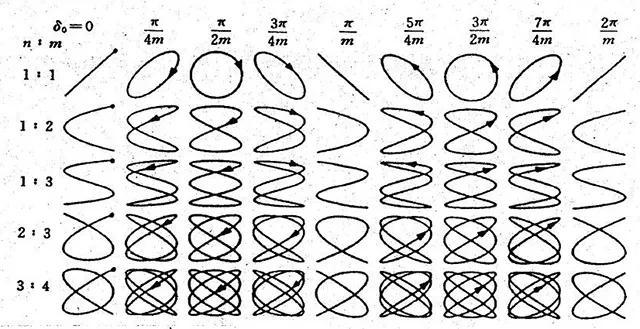
\includegraphics[width=\textwidth]{image/lisaru.jpg}
\end{center}

复数方法的真正价值不在于简化计算，而在于提供几何直觉：$Z(t)$ 不过是两个反向旋转矢量的和，椭圆的形状完全由这两个矢量的长度和夹角决定。一旦你接受了这个图像，你甚至不需要记住那个椭圆方程——你可以在脑子里“看见”两个旋转矢量，从而立即知道轨迹是椭圆、直线还是圆。这正是费曼所说的“理解”与“计算”的区别。







\bigskip

还有最后一种情况，如果一列向右的波和一列向左的波相遇，频率和振幅相同：
\[
\tilde{y} = A e^{i(kx-\omega t)} + A e^{i(-kx-\omega t)} = A e^{-i\omega t}\left(e^{ikx}+e^{-ikx}\right) = 2A\cos(kx)\, e^{-i\omega t}.
\]
取实部：
\[
y = 2A\cos(kx)\cos(\omega t).
\]
注意这个形式：时间和空间彻底分家了。

\begin{wrapfigure}{L}{0.32\textwidth}
  \begin{center}
    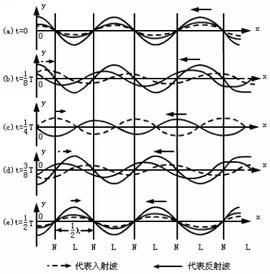
\includegraphics[width=0.3\textwidth]{image/standwav.png}
  \end{center}
    \caption{反射波的驻波}
    \label{fig:standwav}
    \vspace{20pt}
\end{wrapfigure}

每个点$x$都以$\cos(\omega t)$的频率上下振动，但振幅是$2A\cos(kx)$，随位置变化。有些点——$\cos(kx)=0$的点——永远不动，叫波节；有些点——$\cos(kx)=\pm1$的点——振幅最大，叫波腹。相邻波节的距离是半个波长。

驻波不传播能量，只是能量在波节之间来回震荡。这是有限系统中波动的标准形态。驻波一般出现在波与反射波的自干涉，如图\ref{fig:standwav}，这就像拿一把吉他，两端固定的弦，边界条件要求两端必须是波节，所以弦长必须正好是半波长的整数倍：
\[
L = n\frac{\lambda_n}{2}, \quad n=1,2,3,\ldots
\]
允许的频率是离散的：
\[
f_n = \frac{v}{\lambda_n} = n\frac{v}{2L}.
\]
$n=1$叫基频，决定你听到的音高；$n\ge2$叫泛音，决定音色。这就是为什么一根弦能发出美妙的声音——不是因为它的形状复杂，而是因为它只能以这些特定的模式振动。你按在不同的位置，就是改变了有效的$L$，从而改变了基频。

接下来我们不写数学了，来写物理中关于几何光学的部分。

\section{几何光学}

\textbf{惠更斯-菲涅尔原理}（Huygens-Fresnel principle）是波动光学的基石，它将惠更斯的几何作图法与菲涅尔的干涉思想融为一体。


\textbf{惠更斯原理}（1678年）指出：
\begin{quote}
介质中任意时刻的波阵面上的每一点，都可以看作是一个新的次波源，发出球面次波；其后任一时刻，这些次波的包络面就是新的波阵面。
\end{quote}

现在我们回到惠更斯原理本身，用它来推导反射定律。考虑一列平面波入射到平面反射面 $MN$ 上。设 $t=0$ 时刻，波阵面到达 $AB$ 位置。根据惠更斯原理，$A$ 点先成为次波源，发出球面次波；当 $B$ 点到达反射面 $B'$ 时，从 $A$ 点发出的次波已经传播了一段距离。通过几何作图（图\ref{fig:reflection}）可得：
\begin{itemize}
    \item 入射角 $i$ 等于反射角 $r$，即 $i = r$。
    \item 入射光线、反射光线和法线在同一平面内。
\end{itemize}
这就是\textbf{反射定律}。


设平面波从介质1（波速 $v_1$）进入介质2（波速 $v_2$）。$t=0$ 时刻，波阵面为 $AB$，$A$ 点首先到达界面。此后，$A$ 点在介质2中发出次波，而 $B$ 点仍在介质1中向界面运动。当 $B$ 点到达界面 $B'$ 时，从 $A$ 点发出的次波已在介质2中传播了 $v_2 \cdot \Delta t$ 的距离，其中 $\Delta t$ 是 $B$ 到 $B'$ 所需时间。

由几何关系可得：
\[
\frac{\sin i}{\sin r} = \frac{v_1}{v_2}.
\]
引入折射率 $n = c/v$（$c$ 为真空中的光速），则上式化为\textbf{斯涅耳定律}：
\[
n_1 \sin i = n_2 \sin r.
\]

\begin{figure}[H]
\centering
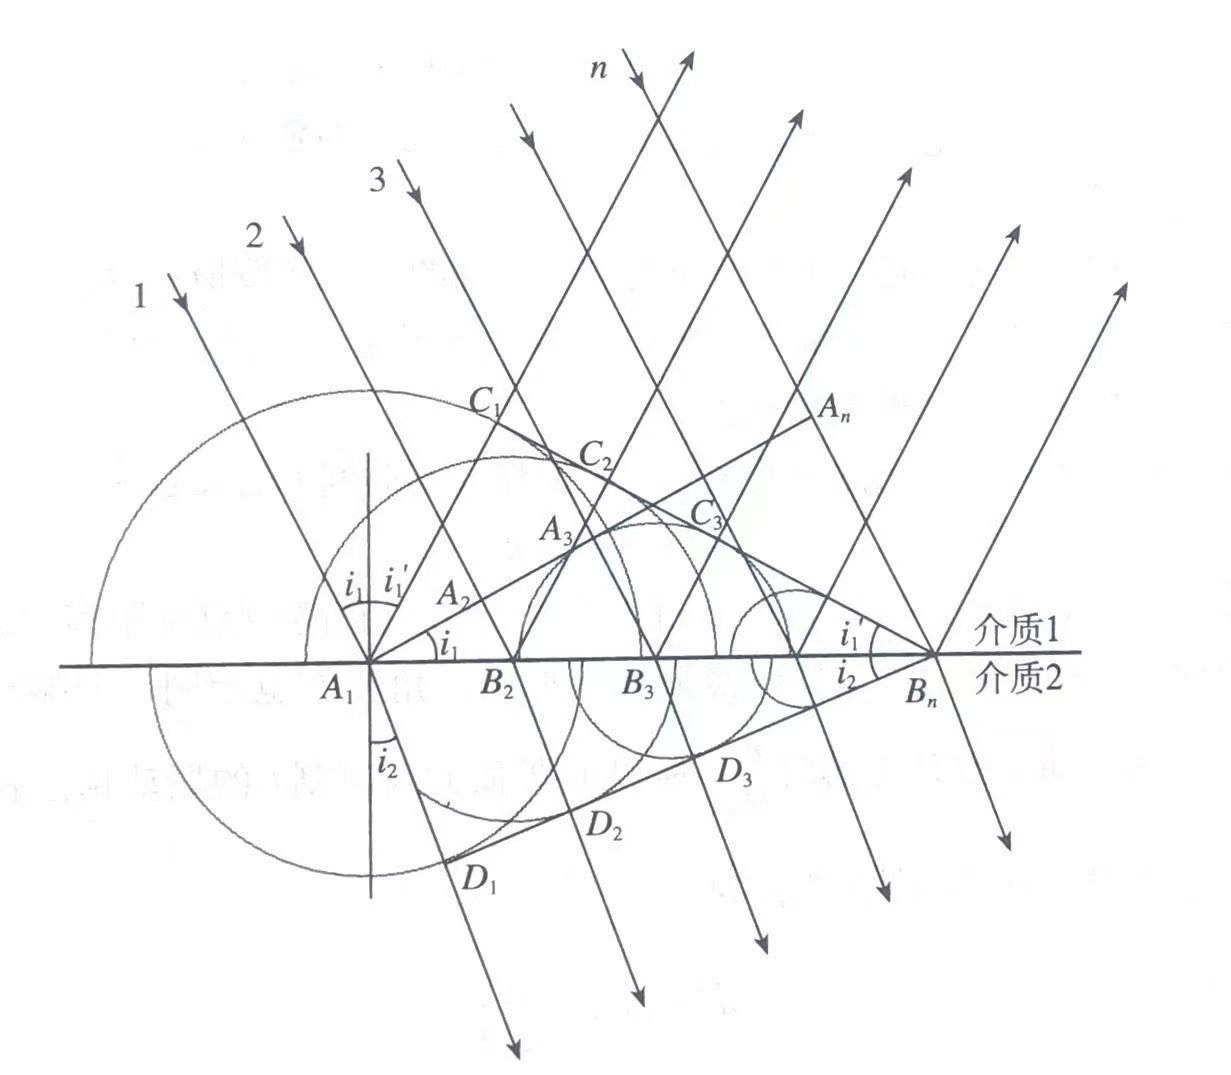
\includegraphics[width=0.62\textwidth]{image/fanshe.jpg}
\caption{反射定律与折射定律}
\label{fig:fanshezheshe}
\end{figure}

这个原理成功地解释了波的反射和折射，但它有一个根本的缺陷：它只能告诉你波“往哪里走”，却无法告诉你“每个方向有多少光强”——它只给出了波前的几何位置，却没有给出振动的振幅分布。

\textbf{菲涅尔}（1818年）对惠更斯原理做出了关键性的补充：
\begin{quote}
空间任意一点的光振动，是波阵面上所有次波源发出的次波在该点相干叠加的结果。
\end{quote}
这就是\textbf{惠更斯-菲涅尔原理}的核心：波在传播过程中，波阵面上的每一点都成为一个相干次波源，这些次波在空间相遇时会发生干涉，而观察到的光场就是所有次波干涉叠加的总效果。

\begin{wrapfigure}{L}{0.32\textwidth}
    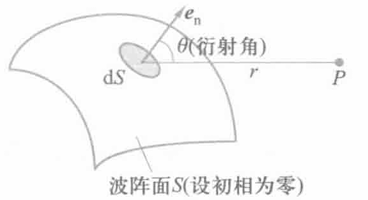
\includegraphics[width=0.32\textwidth]{image/SigmaP.png}
    \caption{波阵面为 $\Sigma$在空间某点 $P$ 产生的干涉}
    \caption{反射波的驻波}
    \label{fig:fanshezheshe}
    \vspace{20pt}
\end{wrapfigure}

设某一时刻的波阵面为 $\Sigma$，其上任意面元 $d\Sigma$ 可以看作一个次波源。该面元在空间某点 $P$ 产生的振动可写为：
\[
dE(P) = K(\theta) \cdot \frac{A}{r} \cdot \cos(\omega t - kr) \cdot d\Sigma,
\]
其中，$A$ 是波阵面上次波源的振幅；，$r$ 是面元到 $P$ 点的距离；， $k = 2\pi/\lambda$ 是波数；， $K(\theta)$ 是\textbf{倾斜因子}，它描述了次波振幅随方向的变化：$\theta = 0$ 时（即沿波传播方向）$K(\theta)$ 最大；$\theta = \pi/2$ 时 $K(\theta)=0$，即次波不会向后传播。$P$ 点的总振动就是整个波阵面上所有面元贡献的叠加：
\[
E(P) = \iint_{\Sigma} K(\theta) \frac{A}{r} \cos(\omega t - kr) \, d\Sigma.
\]


惠更斯-菲涅尔原理统一了几何光学和波动光学：
\begin{itemize}
    \item 在 $\lambda \to 0$ 的极限下，干涉效应消失，波动光学退化为几何光学，惠更斯原理解释了光的直线传播、反射和折射；
    \item 当波长有限时，惠更斯-菲涅尔原理能够解释衍射现象（如圆孔衍射、单缝衍射、圆屏衍射中的泊松亮斑）；
    \item 它是基尔霍夫衍射理论（从波动方程出发的严格理论）的物理雏形，也是费曼路径积分在经典波动光学中的先声。
\end{itemize}


\subsection{光程与费马原理}

在折射定律中，我们看到了速度比等于折射率之比。这提示我们，光在介质中的行为应该与“路径长度乘以折射率”有关。于是有了\textbf{光程}（Optical Path Length, OPL）的定义：
\[
L = \sum_i n_i d_i = \int n \, ds.
\]
物理意义：光在介质中传播的路程乘以折射率，等于光在真空中相同时间内传播的距离。光程把不同介质中的传播统一折算成真空中的传播。

\textbf{费马原理}（Fermat's principle）是说：
\begin{quote}
光从一点到另一点的实际路径，其光程取极值（通常为极小值）。
\end{quote}

由费马原理可以：
\begin{itemize}
    \item 再次导出反射定律和折射定律；
    \item 推导透镜成像公式；
    \item 理解光在渐变折射率介质中的弯曲传播。
\end{itemize}

\subsection{半波损失}

\textbf{当光从光疏介质（折射率小）射向光密介质（折射率大）并在界面上反射时，反射光的相位会发生$\pi$的突变}，相当于多走了半个波长。这就是\textbf{半波损失}。考虑光垂直入射到介质界面。反射系数为
\[
r = \frac{n_1 - n_2}{n_1 + n_2}.
\]
\begin{itemize}
    \item 当$n_1 < n_2$（光疏到光密）时，$r<0$，表示反射光电场方向与入射光相反，即相位突变$\pi$，对应光程增加$\lambda/2$。
    \item 当$n_1 > n_2$（光密到光疏）时，$r>0$，无相位突变，无半波损失。
\end{itemize}

这一结论在干涉现象中至关重要：在计算光程差时，每发生一次“光疏→光密”的反射，就要加上或减去$\lambda/2$。


\subsection{半波面法：理解单缝衍射的直观图像}

\begin{figure}[H]
\centering
\begin{subfigure}[b]{\textwidth}
    \centering
    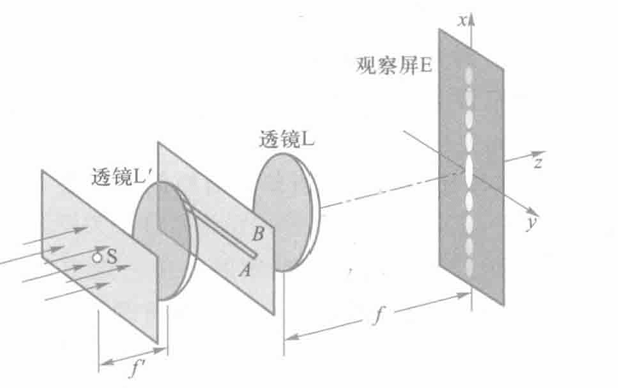
\includegraphics[width=0.6\textwidth]{image/Fraunhofer1.png}
    \caption{夫琅禾费衍射装置}
    \label{fig:Fraunhofer1}
\end{subfigure}

\vspace{1em}

\begin{subfigure}[b]{\textwidth}
    \centering
    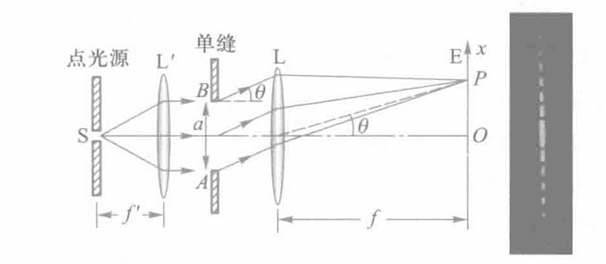
\includegraphics[width=0.6\textwidth]{image/Fraunhofer2.png}
    \caption{夫琅禾费衍射装置光路}
    \label{fig:Fraunhofer2}
\end{subfigure}
\caption{夫琅禾费衍射}
\label{fig:michelson}
\end{figure}

半波面法是一种不使用复杂积分，仅通过几何分割和波动叠加思想来分析单缝衍射图样的经典方法。其核心在于：将单缝处的波前分割成若干个面积相等、但到观察点光程差依次相差半个波长的窄带——这些窄带被称为“半波面”。

当平行光垂直照射到宽度为 \(a\) 的单缝上时，缝所在平面成为一个新的子波源。我们关注屏幕上某一点 \(P\) 的光强。从缝的上、下边缘发出的光到达 \(P\) 的光程差为 \(\Delta = a \sin\theta\)，其中 \(\theta\) 是衍射角。

\begin{figure}[H]
\centering
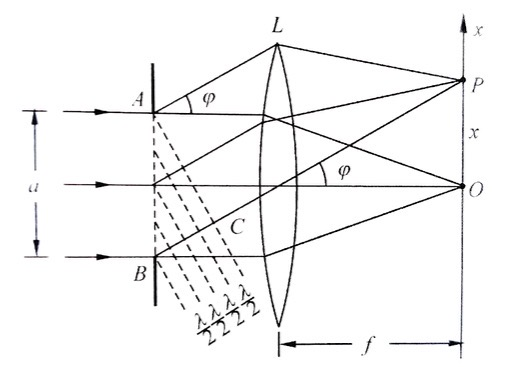
\includegraphics[width=0.62\textwidth]{image/0.5wave.jpg}
\caption{半波面法}
\label{fig:fanshezheshe}
\end{figure}

半波面法其实非常简单，虽然上课时候我没听明白（骗你的，大学生听什么课），这个方法的核心就是惠更斯-菲涅尔原理，废话，它将单缝沿着与缝长垂直的方向（即宽度方向）等分成许多细长的窄带。每个窄带视为发射振幅相同的子波源。相邻窄带到 \(P\) 点的光程差相等。当这个光程差恰好等于半波长 \(\lambda/2\) 时，这两条窄带发出的光在 \(P\) 点就会完全抵消（相位相反，振幅相消）。因此，我们把缝宽 \(a\) 按光程差每 \(\lambda/2\) 一段进行划分。每一段对应的缝宽区域就是一个“半波面”。

假设缝两边缘的光程差也就是$BC$段长度，为 \(a\sin\theta = m\cdot\frac{\lambda}{2}\)。那么半波面的总数 \(N\) 就等于 \(m\)：
\begin{itemize}
    \item 如果 \(N\) 是偶数（即 \(a\sin\theta = 2k\cdot\frac{\lambda}{2} = k\lambda\)），那么半波面两两成对抵消，\(P\) 点光强为极小（暗纹）。
    \item 如果 \(N\) 是奇数（即 \(a\sin\theta = (2k+1)\cdot\frac{\lambda}{2}\)），那么会剩下一个半波面的光无法被抵消，从而形成亮纹（但不是最亮，强度随 \(k\) 增大而减弱）。
    \item 如果 \(N\) 很大（缝很宽）：近于几何光学直线传播。
    \item 如果 \(N\) 很小（缝很窄）：中央亮斑极大加宽。
\end{itemize}
特别地，当 \(\theta=0\) 时，光程差为0，所有半波面的光在 \(P\) 点同相位叠加，形成最亮的中央主极大。

半波面法本质上是一种惠更斯-菲涅耳原理的直观近似。它避免了菲涅耳积分，却抓住了波动干涉中最核心的因素——光程差导致的相位差。通过简单的“成对相消”或“单数残留”模型，半波面法能够清晰解释：
\begin{itemize}
    \item 中央条纹最亮、最宽；
    \item 暗纹条件：\(a\sin\theta = k\lambda\)（\(k=\pm1,\pm2,\dots\)）；
    \item 明纹大致位置：\(a\sin\theta = (2k+1)\frac{\lambda}{2}\)；
    \item 随着衍射级次 \(k\) 增大，光强迅速衰减（因为剩余的半波面宽度变窄）。
\end{itemize}
虽然半波面法简洁易懂，但它只是一种近似。严格的光强分布由夫琅禾费衍射积分给出：
\[
I(\theta)=I_0\left(\frac{\sin\beta}{\beta}\right)^2,\quad \beta=\frac{\pi a\sin\theta}{\lambda}
\]
该函数表明：偶数个半波面对应 \(I=0\)，奇数个半波面对应次极大，但次极大的确切位置与 \((2k+1)\frac{\lambda}{2}\) 略有偏差（例如第一级次极大实际在 \(\beta\approx 1.43\pi\) 处，对应 \(a\sin\theta\approx 1.43\lambda\)，而非 \(1.5\lambda\)）。因此，半波面法适合定性理解与初步估算，精确计算仍需依靠积分公式。

\begin{figure}[H]
\centering
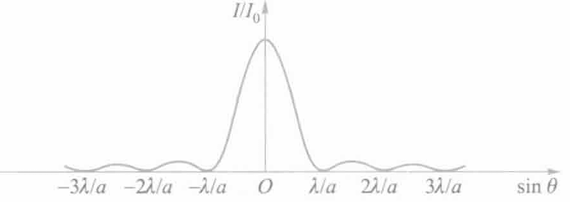
\includegraphics[width=0.62\textwidth]{image/Fraunhofer3.png}
\caption{衍射图样}
\label{fig:Fraunhofer3}
\end{figure}

傍轴近似下，明暗纹坐标就是$sin \theta$乘以到焦平面的距离$f$了。

\subsection{圆孔衍射与艾里斑：从半波带到贝塞尔函数}

圆孔衍射是光学系统分辨本领的理论基石。与单缝衍射的“一维分割”不同，圆孔的对称性使得其衍射图样呈现出同心圆环结构，中心亮斑被称为\textbf{艾里斑}。我们仍可采用类似“半波面”的直观思想来理解其形成，但数学描述需借助贝塞尔函数。

\begin{figure}[H]
\centering
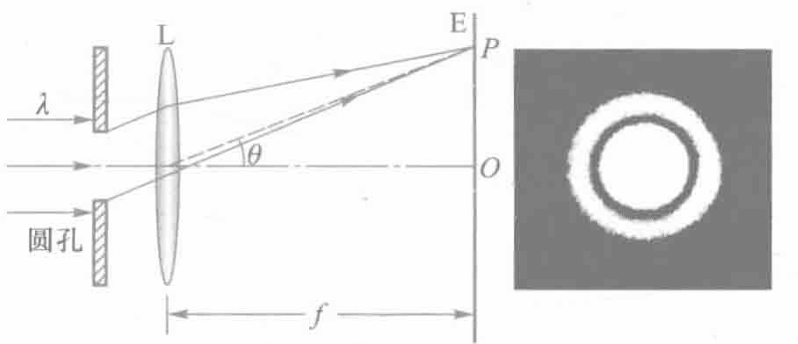
\includegraphics[width=0.55\textwidth]{image/Airy_disk.png}
\caption{圆孔夫琅禾费衍射图样（艾里斑）}
\label{fig:airy_disk}
\end{figure}

对于宽度为 \(a\) 的单缝，我们沿直线方向将波前分割为平行的窄带。对于直径为 \(D\) 的圆孔，对称性要求我们将孔径分割为一系列\textbf{同心圆环带}。考虑屏幕上衍射角为 \(\theta\) 的某点 \(P\)，从圆孔中心到边缘的光程差为：
\[
\Delta = D\sin\theta
\]
我们按光程差每 \(\lambda/2\) 为间隔，将圆孔划分为 \(N\) 个同心半波带。第一个半波带是中心处半径为 \(r_1\) 的圆斑，第二个是宽度为 \((r_2-r_1)\) 的圆环，依此类推。相邻半波带发出的子波在 \(P\) 点的相位相反，因此也会发生两两相消。

然而，与单缝情况有两点关键不同：
\begin{itemize}
    \item \textbf{面积权重不同}：圆环带的面积随半径线性增大（\( \mathrm dA = 2\pi r\,\mathrm dr \)），外圈半波带贡献的子波振幅更大，不能简单视为等振幅成对抵消；
    \item \textbf{相位分布复杂}：各环带内不同方位角的子波到达 \(P\) 点的相位并非一致，需对整个圆面积分，这使得严格求解依赖于贝塞尔函数。
\end{itemize}

夫琅禾费圆孔衍射的振幅分布可由圆孔面上各子波源的积分给出。设圆孔半径为 \(R = D/2\)，观察点 \(P\) 的衍射角为 \(\theta\)，则复振幅为：
\[
U(\theta) \propto \int_0^R \int_0^{2\pi} e^{ik\rho\sin\theta\cos\phi} \,\rho\,\mathrm d\rho\,\mathrm d\phi
\]
其中 \(\rho\) 是圆孔面上的极径，\(\phi\) 是极角，\(k = 2\pi/\lambda\)。该二重积分结果为：
\[
U(\theta) \propto \frac{2J_1(ka\sin\theta)}{ka\sin\theta}
\]
其中 \(J_1\) 为\textbf{第一类一阶贝塞尔函数}。因此，圆孔衍射的光强分布为：
\[
I(\theta) = I_0 \left[\frac{2J_1(x)}{x}\right]^2, \quad x = \frac{\pi D}{\lambda}\sin\theta
\]
这一表达式与单缝衍射的 \( \left(\sin\beta/\beta\right)^2 \) 形式相似，但分子由正弦函数换成了贝塞尔函数 \(J_1(x)\)。


贝塞尔函数 \(J_1(x)\) 的第一个零点位于 \(x = 3.8317\)。由此可得中央亮斑（艾里斑）边缘对应的衍射角：
\[
\sin\theta = \frac{3.8317}{\pi}\cdot\frac{\lambda}{D} \approx 1.22\frac{\lambda}{D}
\]
这就是瑞利判据给出的\textbf{最小分辨角}。中央亮斑集中了约 \(84\%\) 的衍射光能，其角半径由 \(1.22\lambda/D\) 决定。随着 \(x\) 增大，\(J_1(x)\) 呈现衰减振荡，对应着各级暗环与次极大亮环：
\begin{itemize}
    \item 暗环条件：\(J_1(x) = 0\)，即 \(x = 3.8317,\, 7.0156,\, 10.1735,\, \dots\)
    \item 次极大位置：约在 \(x = 5.136,\, 8.417,\, 11.620,\, \dots\)，对应强度依次迅速衰减。
\end{itemize}

\begin{wrapfigure}{L}{0.32\textwidth}
    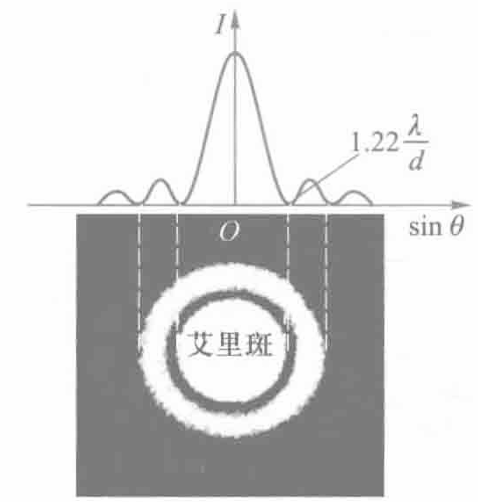
\includegraphics[width=0.32\textwidth]{image/Circular_diffraction_pattern.png}
    \caption{圆孔夫琅禾费衍射截面光强分布（艾里斑与衍射环）}
    \label{fig:circular_diffraction}
    %\vspace{10pt}
\end{wrapfigure}

与单缝衍射的明暗条纹相比，圆孔衍射图样具有以下特点：
\begin{itemize}
    \item 中央亮斑（艾里斑）占据最大亮度与最宽角半径；
    \item 周围环绕明暗相间的同心圆环，但环纹亮度随级次衰减更快；
    \item 第一级暗环对应的 \(1.22\lambda/D\) 定义了光学系统极限分辨能力。
\end{itemize}

半波面法的直观图像虽能解释“成对相消”的基本物理图像，但由于圆孔的二维对称性，严格的光强分布必须依赖贝塞尔函数。因此，圆孔衍射的最小分辨角 \(1.22\lambda/D\) 正是贝塞尔函数第一个零点 \(3.8317\) 与圆周率 \(\pi\) 之比——这是二维圆孔衍射的本质特征，而非对单缝公式的简单修正。

傍轴近似下，焦平面上艾里斑的线半径为：
\[
r = f\cdot\theta \approx 1.22\frac{f\lambda}{D}
\]
其中 \(f\) 为透镜焦距。这一表达式直接决定了望远镜、显微镜等光学仪器的理论分辨极限。

\subsection{光栅衍射：从单缝到多缝的干涉调控}

半波面法为理解单缝衍射提供了清晰的物理图像，而光栅衍射则是这一思路的自然延伸与重要应用。光栅由大量等宽、等间距的平行狭缝构成，设缝宽为 \(a\)，相邻狭缝中心间距为 \(d\)（称为光栅常数），总缝数为 \(N\)。当平面波垂直入射时，每个狭缝自身产生单缝衍射图样，而不同狭缝之间又发生多光束干涉。因此，光栅衍射是单缝衍射与多缝干涉联合作用的结果。

\begin{figure}[H]
\centering
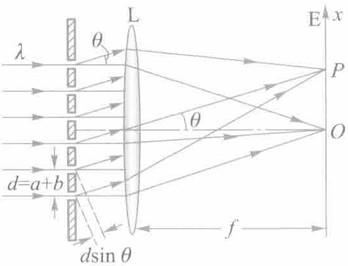
\includegraphics[width=0.62\textwidth]{image/grating.png}
\caption{光栅衍射光路图}
\label{fig:grating}
\end{figure}

多缝干涉的主极大条件为各缝发出的光在观察点同相位叠加。相邻狭缝的光程差为 \(d\sin\theta\)，对应的相位差为 \(\Delta\varphi = \frac{2\pi}{\lambda} d\sin\theta\)。当 \(\Delta\varphi = 2k\pi\) 时，所有缝的振动同相位叠加，形成主极大，由此得到\textbf{光栅方程}：
\[
d\sin\theta = k\lambda \quad (k = 0, \pm 1, \pm 2, \dots)
\]
主极大在屏上的位置为 \(x = k\lambda \dfrac{f}{d}\)，其强度为单缝衍射在该方向光强的 \(N^2\) 倍。主极大的位置仅由光栅常数 \(d\) 决定，与缝宽 \(a\) 无关。

然而，每个狭缝自身的衍射特性会对总光强产生调制作用。由半波面法可知，当衍射角 \(\theta\) 满足 \(a\sin\theta = m\lambda\)（\(m = \pm 1, \pm 2, \dots\)）时，单缝在该方向的光强为零。这一条件构成了光栅衍射强度的“包络线”——即使多缝干涉在该方向本应出现主极大，若恰好落在单缝衍射的零点处，该级主极大也将消失。这种干涉主极大与单缝衍射暗纹重合而导致主极大不出现的现象称为\textbf{缺级}。联立光栅方程与单缝暗纹条件：
\[
\begin{cases}
d\sin\theta = k\lambda & \text{（干涉主极大）}\\
a\sin\theta = m\lambda & \text{（单缝暗纹）}
\end{cases}
\]
可得缺级条件为 \(\dfrac{d}{a} = \dfrac{k}{m}\)，即当光栅常数与缝宽之比等于两个整数之比时，第 \(k\) 级主极大缺级。例如，若 \(d/a = 2\)，则 \(k = \pm 2, \pm 4, \pm 6, \dots\) 级缺级；若 \(d/a = 3\)，则 \(k = \pm 3, \pm 6, \pm 9, \dots\) 缺级；若 \(d/a = 3/2\)，则 \(k = \pm 3, \pm 6, \pm 9, \dots\) 缺级。

除了缺级现象，光栅常数 \(d\) 和缝宽 \(a\) 还对条纹的整体分布产生不同影响。光栅方程 \(d\sin\theta = k\lambda\) 表明，\(d\) 决定了主极大的疏密：\(d\) 越大，相邻主极大的角间距 \(\Delta\theta \approx \lambda/(d\cos\theta)\) 越小，条纹越密集；反之 \(d\) 越小，条纹越稀疏。而缝宽 \(a\) 则决定了单缝衍射包络的宽度，中央明纹的半角宽度为 \(\lambda/a\)，\(a\) 越小，包络越宽，中央包络内包含的主极大数目也就越多。

缝数 \(N\) 虽然不改变主极大的位置，但显著影响条纹的精细结构。相邻主极大之间有 \(N-1\) 条暗纹和 \(N-2\) 个次极大，主极大的半角宽度 \(\Delta\theta \propto \dfrac{\lambda}{Nd\cos\theta}\)，因此 \(N\) 越大，条纹越细锐，同时主极大强度 \(\propto N^2\)（但受单缝衍射包络调制）。当 \(N\) 很大时，主极大变成极其尖锐的亮线，这正是光栅具有高分光能力的原因。这种缝间干涉的物理本质可以用半波面法的思想来类比：将 \(N\) 条缝看作 \(N\) 个等间距子波源，当 \(d\sin\theta = k\lambda\) 时，所有缝到达观察点的光程差为 \(\lambda\) 的整数倍，相位相同，形成主极大；当光程差偏离恰好一个 \(\lambda/N\) 时，\(N\) 个振动矢量围成近乎闭合的正多边形，合振幅急剧减小，这正是条纹尖锐的根源。

作为精密的分光元件，光栅的角色散率和色分辨本领分别为：
\[
\frac{\mathrm{d}\theta}{\mathrm{d}\lambda} = \frac{k}{d\cos\theta}, \qquad
R = \frac{\lambda}{\Delta\lambda} = kN,
\]
表明缝数 \(N\) 越多、级次 \(k\) 越高，分辨相邻波长细节的能力就越强。

\begin{figure}[H]
\centering
\begin{subfigure}[b]{\textwidth}
    \centering
    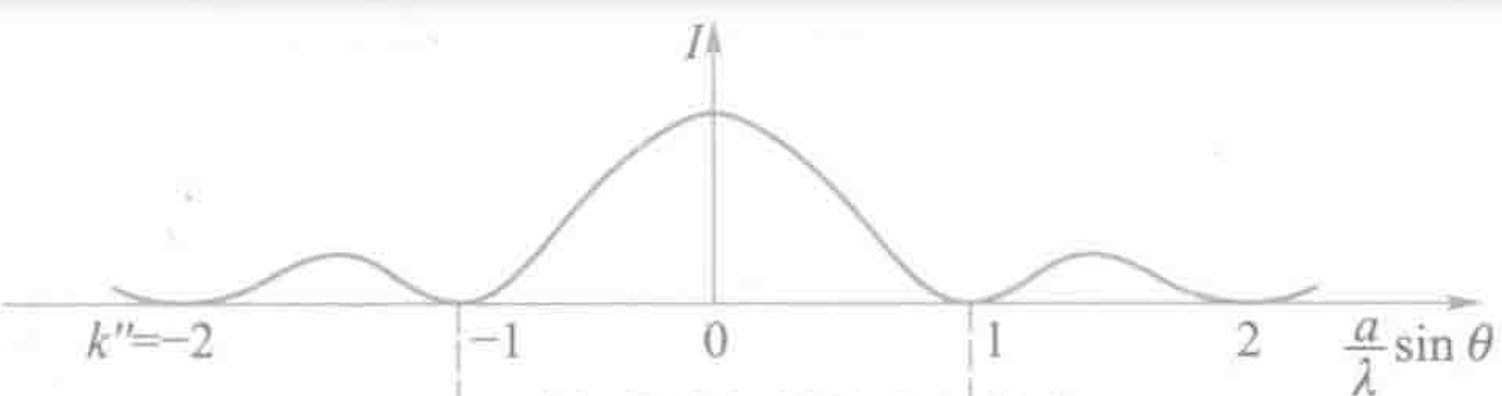
\includegraphics[width=0.8\textwidth]{image/grating1.png}
\end{subfigure}

\begin{subfigure}[b]{\textwidth}
    \centering
    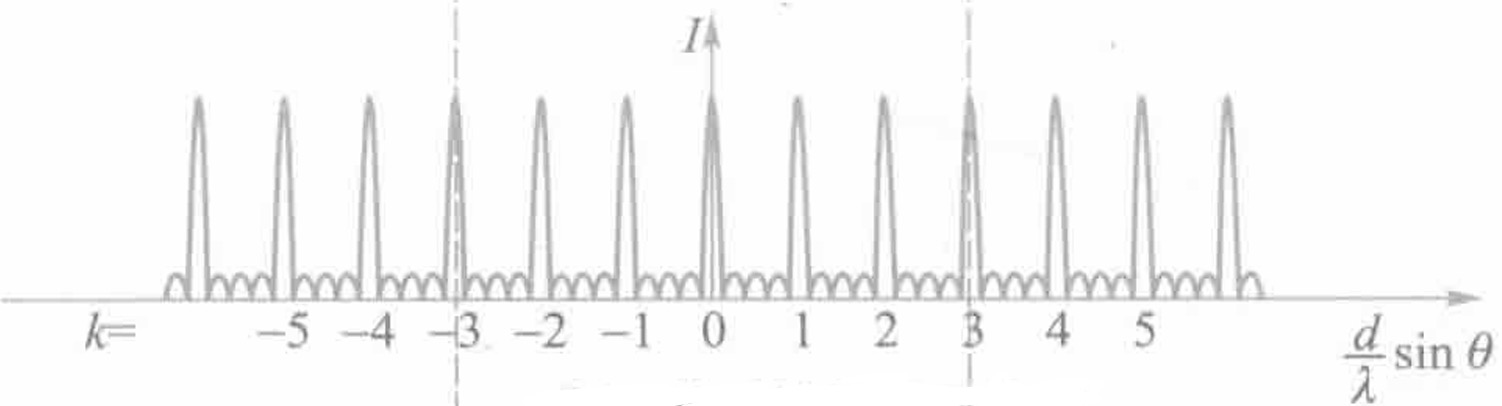
\includegraphics[width=0.8\textwidth]{image/grating2.jpg}
\end{subfigure}

\begin{subfigure}[b]{\textwidth}
    \centering
    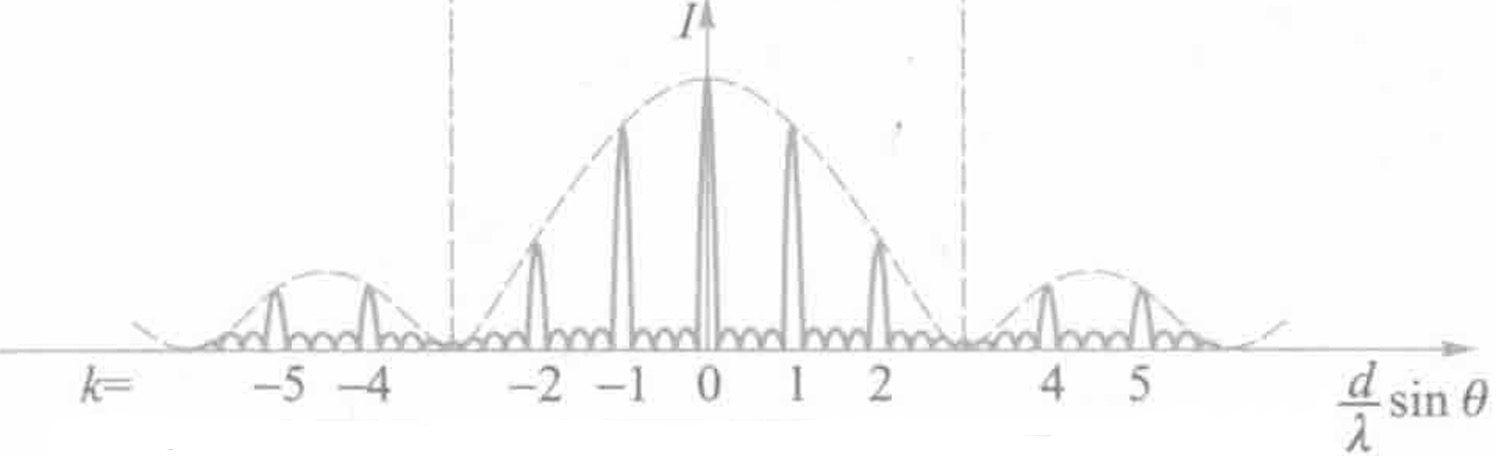
\includegraphics[width=0.8\textwidth]{image/grating3.jpg}
\end{subfigure}

\caption{夫琅禾费衍射}
\label{fig:grating123}
\end{figure}

为便于系统理解，将上述关系总结如下：

\begin{table}[H]
\centering
\begin{tabular}{|c|c|c|}
\hline
\textbf{物理量} & \textbf{公式} & \textbf{对光栅衍射的解释} \\
\hline
单缝暗纹 & \(a\sin\theta = m\lambda\) & 衍射包络的零点，导致缺级 \\
\hline
干涉主极大（光栅方程） & \(d\sin\theta = k\lambda\) & 主极大位置，由 \(d\) 决定疏密 \\
\hline
缺级条件 & \(d/a = k/m\) & 干涉峰恰好落在衍射零点 \\
\hline
缝数 \(N\) & — & \(N\) 越大，主极大越锐，极小越多 \\
\hline
\end{tabular}
\end{table}

综上，半波面法所奠基的“分割波前→相位差→叠加结果”的分析框架，在光栅衍射中升华为“单缝衍射包络 + 多缝干涉结构”的乘积图像。半波面法导出的单缝暗纹条件 \(a\sin\theta = m\lambda\) 与光栅方程 \(d\sin\theta = k\lambda\) 相配合，能够完整解释光栅衍射的“包络-峰”结构、缺级、条纹密度与条纹锐度等全部核心现象。这一图像不仅贯穿于夫琅禾费衍射的理论核心，也是设计光谱仪、光栅单色仪等现代光学仪器的物理基础，体现了从单缝到多缝、从简单到复杂的物理思想的一脉相承。


\subsection{光学透镜}

在近轴近似（$\sin\theta \approx \theta$）下，利用光程相等的费马原理，可以推导出透镜成像公式。


对于单个球面（曲率半径$R$），两侧介质折射率分别为$n_1$和$n_2$，物距为$u$，像距为$v$，有：
\[
\frac{n_1}{u} + \frac{n_2}{v} = \frac{n_2 - n_1}{R}.
\]
符号规则：光线从左向右传播，物距$u$在左侧取正，曲率中心在右侧时$R>0$，反之为负。


对于放在空气（$n=1$）中的薄透镜，由两个球面组合可得\textbf{薄透镜公式}：
\[
\frac{1}{u} + \frac{1}{v} = \frac{1}{f},
\]
其中$f$为焦距，由\textbf{透镜制造者公式}给出：
\[
\frac{1}{f} = (n - 1)\left( \frac{1}{R_1} - \frac{1}{R_2} \right).
\]
$R_1$和$R_2$分别为透镜两个球面的曲率半径，符号按光线入射顺序确定。



\subsection{光学干涉}


当两束光满足频率相同、振动方向相同、相位差恒定时，它们会发生干涉，产生稳定的明暗相间条纹。为了获得稳定的相干光，一般有分波振面法和分波振幅法。


分波振幅法就是将一束光的振幅（能量）分成两部分（或多部分），让它们经过不同路径后再相遇，产生干涉。相比于分波振面法，分波振幅法的家族则更为庞大，主要分为等厚薄膜干涉和等倾薄膜干涉。

等厚干涉的核心特征就是通过厚度相等的介质的光形成一道干涉条纹，一般的等厚干涉如图\ref{fig:denghou}。

\begin{wrapfigure}{R}{0.4\textwidth}
  \begin{center}
    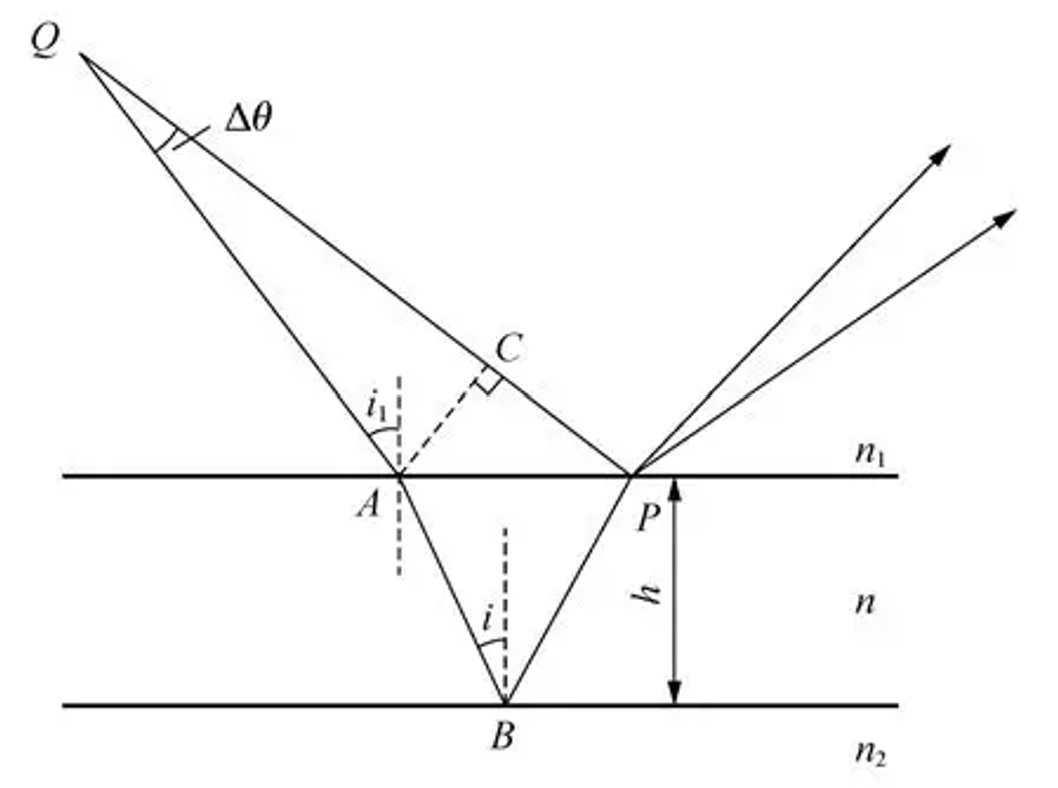
\includegraphics[width=0.4\textwidth]{image/denghou.png}
  \end{center}
    \caption{等厚干涉}
    \label{fig:denghou}
    \vspace{20pt}
\end{wrapfigure}

当一束平行光垂直照射到厚度不均匀的透明薄膜上时，从薄膜上下表面反射的两束光发生干涉。若薄膜的折射率 $n$ 均匀，则两束反射光的光程差为：
\[
\delta = 2nd + \frac{\lambda}{2} \quad \text{或} \quad \delta = 2nd,
\]
其中 $\frac{\lambda}{2}$ 项取决于半波损失是否发生（上下表面反射共产生奇数次还是偶数次相位突变）。

从我们在波的干涉章节讨论知道，相干抵消与否本质就是相位差是否相差半周期，而在这里我们又可以简化为光程差，所以产生干涉的条件就是：
\begin{itemize}
    \item 明纹：$\delta = m\lambda \quad (m = 0,1,2,\dots)$
    \item 暗纹：$\delta = \left(m + \frac12\right)\lambda \quad (m = 0,1,2,\dots)$
\end{itemize}

由于光程差 $\delta$ 仅依赖于薄膜厚度 $d$，因厚度相同的地方对应同一级干涉条纹——这就是“等厚干涉”名字的由来。

典型的等厚干涉装置包括：
\begin{itemize}
    \item \textbf{劈尖}：两平面玻璃一端接触，形成微小夹角的空气楔，条纹为平行直纹；
    \item \textbf{牛顿环}：平凸透镜与平面玻璃接触，形成同心环状空气膜，条纹为同心圆环。
\end{itemize}

等厚干涉的应用包括：测量微小角度、检测表面平整度、测定透镜曲率半径、检验光学元件质量等。

\begin{wrapfigure}{L}{0.37\textwidth}
  \begin{center}
    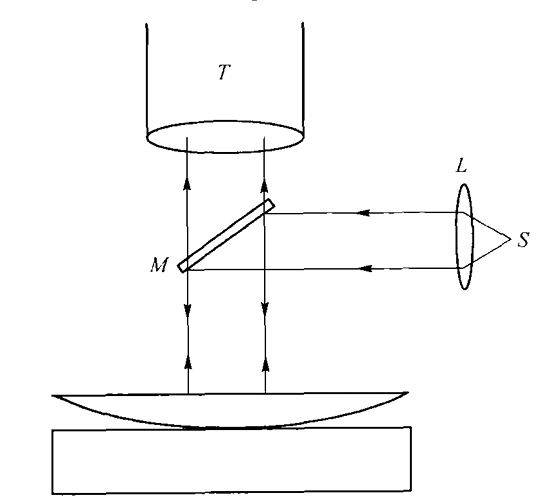
\includegraphics[width=0.35\textwidth]{image/NewtonRing.png}
  \end{center}
    \caption{牛顿环}
    \label{fig:NewtonRing}
    \vspace{20pt}
\end{wrapfigure}
牛顿环干涉装置就是简单的将平凸透镜凸面朝下放在平面玻璃上。平凸透镜和平面玻璃之间形成一层厚度不均的空气膜。用单色光垂直照射，在反射光中可观察到以接触点为中心的同心圆环，这就是牛顿环。干涉之所以形成主要是因为平行光源和反射光在反射镜处产生干涉，二者相比，反射光的光程在半波损失的基础上（从空气进入到玻璃时产生）还叠加空气膜厚度的产生的额外光程，所以光程差（考虑一次半波损失）：
\[
\delta = 2d + \frac{\lambda}{2}.
\]
显然空气膜厚度相等的部分呈现环状分布，从而呈现的干涉条纹也呈现同心圆环的图像，这类似某种等高线。根据勾股定理，我们直接得到空气膜厚$d$与环半径$r$的关系（$R$为透镜曲率半径）：
\[
R^2 = r^2 + (R - d)^2 \longrightarrow r^2 = 2Rd.
\]

用已知量代入之前的干涉条件我们得到：
\begin{itemize}
    \item 明环：$\delta = m\lambda \;\Rightarrow\; r^2 = \left(m - \frac12\right)\lambda R$
    \item 暗环：$\delta = \left(m + \frac12\right)\lambda \;\Rightarrow\; r^2 = m\lambda R$
\end{itemize}

牛顿环装置一般被广泛应用于测定透镜曲率半径、检查光学表面质量、测量微小位移。这个实验也是大学物理实验的常客，只不过并不被大学生们欢迎。

\begin{wrapfigure}{R}{0.5\textwidth}
  \begin{center}
    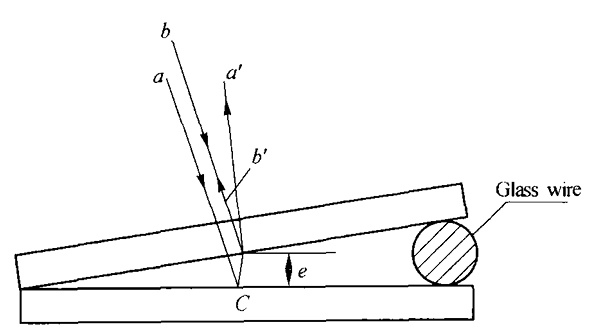
\includegraphics[width=0.48\textwidth]{image/Pijian.png}
  \end{center}
    \caption{劈尖干涉示意图}
    \label{fig:Pijian}
    \vspace{20pt}
\end{wrapfigure}

劈尖干涉的装置也很简单，就是将两片平面玻璃一端接触，另一端垫薄片，从而形成一微小角度的空气楔（劈尖）。用单色光垂直照射，在反射光中看到平行于棱边的等厚干涉条纹。对于劈尖角为$\theta$的劈尖，在傍轴近似（$\sin\theta \approx \theta$）下有膜厚$e = x\theta$（$x$为到棱边的距离），光路$a$和$b$的光程差主要就是在空气隙的部分，在劈尖干涉中，入射光近乎垂直，劈尖角 $\theta$ 很小（通常小于 $1^\circ$）。因此，光线在空气隙中的实际路径长度 $2e/\cos\theta$ 与竖直高度 $2e$ 的差别极小：
\[
\frac{2e}{\cos\theta} = 2e \left(1 + \frac{\theta^2}{2} + \cdots\right) \approx 2e,
\]
其中 $\cos\theta \approx 1 - \theta^2/2$。对于 $\theta = 0.1^\circ$，$\theta^2/2 \approx 1.5\times10^{-6}$，相对误差可忽略。故在傍轴近似下，可直接用 $2e$ 表示空气隙中的光程差，所以光程差（考虑一次半波损失）：
\[
\delta = 2e + \frac{\lambda}{2}.
\]
它的明暗纹条件与牛顿环相同。相邻明纹（或暗纹）对应的厚度差为$\lambda/2$，对应的水平间距为：
\[
\Delta x = \frac{\Delta e}{\theta} =\frac{((m+1) \lambda - \lambda /2)-(m \lambda - \lambda /2)}{2 \theta} = \frac{\lambda}{2\theta}.
\]

这个一般用来测量微小角度或薄片厚度：$\theta = \lambda/(2\Delta x)$，检测表面平整度：条纹弯曲表明表面不平，测量热膨胀系数、透明薄膜厚度等。这点我深有体会，我在做大学物理实验光的干涉的劈尖干涉部分的时候，我组装完装置后做出来的条纹是垂直于劈尖的，当时我叫老师过来，他看了看说：“嗯做的很标准。”然后看了看显微镜：“嗯？！！”后来他和我说，可能是劈尖表面不平整才导致了这样的奇观。

迈克尔逊干涉仪是等倾干涉和等厚干涉的典型装置，它也是通过分振幅的方式产生干涉。


如图\ref{fig:michelson}所示，迈克尔逊干涉仪的主要部件包括：
\begin{itemize}
    \item 一个\textbf{分束器}（半透半反镜）：将入射光分成两束，一束反射（光束1），一束透射（光束2）；
    \item 两个平面反射镜：$M_1$（固定）和 $M_2$（可移动）；
    \item 一个\textbf{补偿板}：使两束光通过玻璃板的次数相同，消除色散影响。
\end{itemize}

\begin{figure}[H]
\centering
\begin{subfigure}[b]{0.45\textwidth}
    \centering
    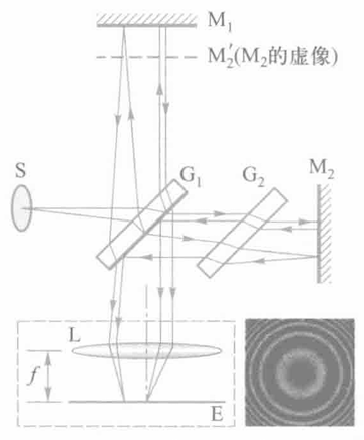
\includegraphics[width=\textwidth]{image/Mchesonint1.png}
    \caption{$M_1$和$M_2$严格垂直时光路示意图及等倾条纹照相}
    \label{fig:michelson1}
\end{subfigure}
\hfill
\begin{subfigure}[b]{0.45\textwidth}
    \centering
    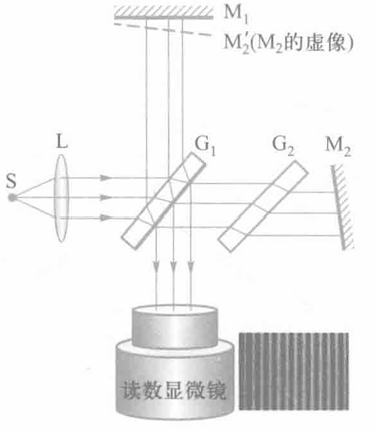
\includegraphics[width=\textwidth]{image/Mchesonint2.png}
    \caption{$M_1$和$M_2$不严格垂直时光路示意图及等厚条纹照相}
    \label{fig:michelson2}
\end{subfigure}
\caption{迈克尔逊干涉仪}
\label{fig:michelson}
\end{figure}


光路如下：从扩展光源发出的光经分束器分成两束——反射光射向 $M_1$，透射光射向 $M_2$。两束光分别被 $M_1$ 和 $M_2$ 反射后返回分束器，再次相遇并发生干涉，进入观察屏。由于分束器的作用，$M_2$ 在半透半反镜中的虚像 $M_2'$ 与 $M_1$ 构成一个\textbf{等效空气膜}。设 $M_1$ 到分束器的距离为 $d_1$，$M_2$ 到分束器的距离为 $d_2$，则等效空气膜的厚度为：
\[
d = d_1 - d_2 \quad (\text{或取绝对值})
\]
当 $M_1$ 和 $M_2'$ 严格平行时，等效为平行平板，产生\textbf{等倾干涉}；当 $M_1$ 和 $M_2'$ 有一微小夹角时，等效为劈尖，产生\textbf{等厚干涉}。
对于等倾干涉（两镜平行）：
\[
\delta = 2d\cos\theta + \frac{\lambda}{2}
\]
其中 $\theta$ 是光线在等效膜中的折射角（空气 $n\approx1$，$\theta$ 近似等于入射角），$\lambda/2$ 来自半波损失（视具体反射情况而定）。

干涉条件：
\begin{itemize}
    \item 明纹：$\delta = m\lambda$（$m$ 为整数）
    \item 暗纹：$\delta = \left(m + \frac12\right)\lambda$
\end{itemize}

对于等厚干涉（两镜有一微小夹角），类似于劈尖：
\[
\delta = 2d + \frac{\lambda}{2}
\]
条纹为平行直纹，间距 $\Delta x = \lambda/(2\theta)$。



\begin{figure}[H]
\centering
\begin{subfigure}[b]{\textwidth}
    \centering
    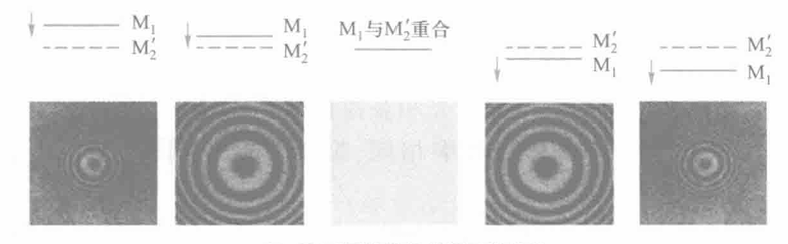
\includegraphics[width=\textwidth]{image/Mchesonint3.png}
    \caption{$M_1$不同位置等倾干涉条纹}
    \label{fig:michelson3}
\end{subfigure}

\vspace{1em}

\begin{subfigure}[b]{\textwidth}
    \centering
    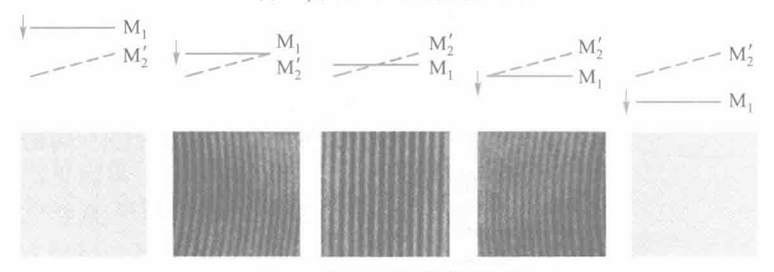
\includegraphics[width=\textwidth]{image/Mchesonint4.png}
    \caption{$M_1$不同位置等厚干涉条纹}
    \label{fig:michelson4}
\end{subfigure}
\caption{迈克尔逊干涉仪干涉条纹}
\label{fig:michelson}
\end{figure}

\begin{itemize}
    \item \textbf{测长度（或位移）}：移动 $M_2$，条纹每变化一级，$M_2$ 移动 $\lambda/2$。因此通过数条纹变化数 $\Delta m$ 可测微小位移：
    \[
    \Delta d = \Delta m \cdot \frac{\lambda}{2}
    \]
    \item \textbf{测折射率}：在光路中插入透明介质，光程差变化引起条纹移动，可反推折射率。
    \item \textbf{测波长}：已知位移，数条纹变化数，可计算 $\lambda$。
    \item \textbf{光谱分析}：通过干涉图样分析光源的频谱成分。
\end{itemize}

\begin{itemize}
    \item 精度极高（可测 $\lambda/2$ 量级的位移）
    \item 既可等倾（两镜平行，扩展光源），也可等厚（两镜有夹角，点光源）
    \item 迈克尔逊-莫雷实验正是用此装置否定了“以太”的存在，为狭义相对论奠定了基础
\end{itemize}

杨氏双缝干涉是最经典的分波阵面干涉实验。一个点光源或线光源发出的光，其波阵面是连续的球面或柱面。如果在波阵面上取两个不同的点（或两个小区域），这两个点发出的光来自同一光源的同一波阵面，因此它们频率相同、相位差恒定（初始相位相同或相差固定值），满足相干条件。简单地说就是单色光通过两条相距$d$的狭缝，在距离为$D$的屏上形成干涉条纹。

\begin{figure}[H]
  \begin{center}
    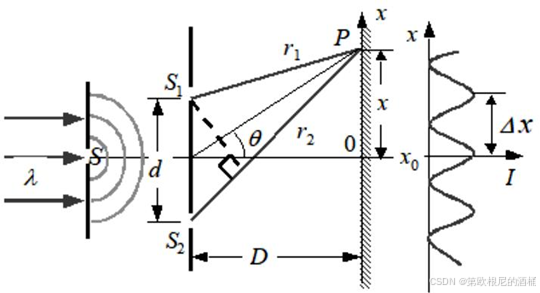
\includegraphics[width=0.5\textwidth]{image/Shuangfeng.png}
  \end{center}
    \caption{双缝干涉示意图}
    \label{fig:Shuangfeng}
\end{figure}

对于杨氏双缝干涉，设双缝间距为 $d$，缝到屏的距离为 $D$，屏上点 $P$ 到中心 $O$ 的距离为 $y$。从两缝 $S_1$ 和 $S_2$ 到 $P$ 的光程差为：
\[
\delta = S_2P - S_1P.
\]
在 $D \gg d$ 且 $D \gg y$ 的条件下（傍轴近似），$S_1P$ 和 $S_2P$ 近似平行，过 $S_1$ 作 $S_2P$ 的垂线 $S_1M$，则 $S_2M = d\sin\theta$，且 $\delta \approx S_2M = d\sin\theta$。又因为 $\theta$ 很小，$\sin\theta \approx \tan\theta = y/D$，故：
\[
\delta = d\sin\theta \approx d \cdot \frac{y}{D}.
\]
其中$y$为屏上位置坐标，$\theta$为衍射角。

干涉条件：
\begin{itemize}
    \item 明纹（相长干涉）：$\delta = m\lambda,\quad m = 0, \pm1, \pm2, \dots$
    \item 暗纹（相消干涉）：$\delta = \left(m + \frac12\right)\lambda,\quad m = 0, \pm1, \pm2, \dots$
\end{itemize}

相邻明纹（或暗纹）之间的间距为：
\[
\Delta y = \frac{\lambda D}{d}.
\]
它的主要\textbf{应用}是测量光波波长、测定微小长度变化，也是干涉仪基础。

此外还有一种它的变形，就是劳埃德镜，通过在两狭缝中心垂直于光屏放置一个反射镜，使得$S_1$和它自己的像作为$S_2$发生干涉，其它的和杨氏干涉一样。

杨氏双缝实验的成功，自然引发了一个深刻的追问：如果我们在波阵面上不只取两个点，而是取无穷多个点，并且让这些点无限密集地排列，会发生什么？

想象一下，我们将双缝换成一块有着无穷多条狭缝的光栅——或者说，干脆把整个波阵面都敞开，不设任何遮挡。当光从光源发出后，波阵面上的每一点都成为次波源，发出球面次波。空间任意一点的振动，就是所有这些次波在该点干涉叠加的结果。

这不就是惠更斯-菲涅尔原理的另一种表述吗？是的。但问题在于：当狭缝数目趋于无穷、缝间距趋于零时，我们实际上是在对波阵面做“连续求和”——也就是积分。光从光源 $S$ 发出，经过某个开孔或障碍物，到达观察点 $P$，其振幅可以写成：
\[
\psi(P) = \iint_{\text{开孔}} \frac{e^{ikr}}{r} \, dS,
\]
其中 $r$ 是波阵面上某点到 $P$ 的距离，$k = 2\pi/\lambda$。这就是菲涅尔-基尔霍夫衍射公式的雏形。

费曼给出了一个更深刻、更统一的视角：把光的传播看作所有可能路径的贡献之和。在经典的双缝实验中，光只有两条路径（$S \to S_1 \to P$ 和 $S \to S_2 \to P$）。当我们把缝增加到 $N$ 条时，光有 $N$ 条路径。当 $N \to \infty$、缝的宽度趋于零时，我们不再有“缝”的概念——光可以从源到屏之间走任意一条路径，每条路径对最终振幅的贡献是一个相位因子 $e^{ikL}$，其中 $L$ 是该路径的光程。

这就是\textbf{费曼路径积分}的核心思想：
\[
\psi(P) \propto \sum_{\text{所有路径}} e^{ikL}.
\]
在经典极限下（$\lambda \to 0$），相位 $kL$ 极大，只有那些使得 $L$ 取极值的路径（即光程取极值的路径）才会相干叠加出一个显著的贡献——这就是费马原理。其他路径的相位快速震荡，相互抵消。

从这个角度看，几何光学（费马原理）只是波动光学（惠更斯-菲涅尔原理）的短波近似，而波动光学又是量子力学中路径积分形式在宏观尺度上的体现。光从双缝到无穷多缝，从离散求和到连续积分，从费马原理到惠更斯-菲涅尔再到路径积分——这是物理学中一个极其优美的一脉相承。

\begin{figure}[H]
\centering
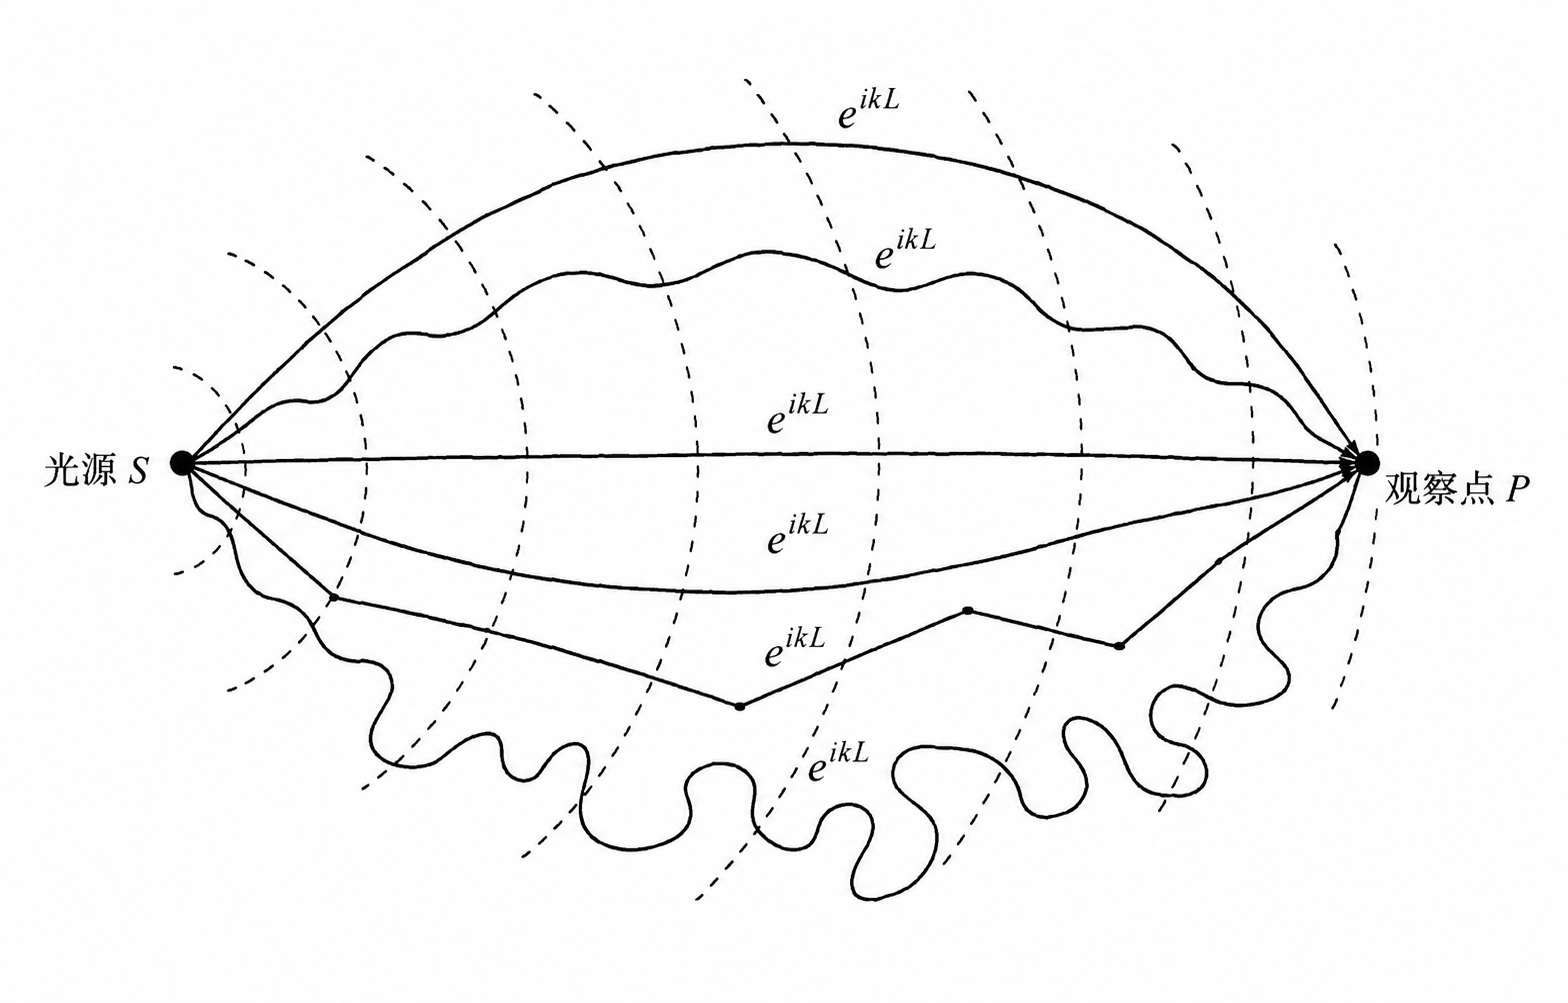
\includegraphics[width=0.6\textwidth]{image/FeynmanPath.png}  % 如果有图的话
\caption{费曼路径积分示意图：光从源 $S$ 到点 $P$ 可以沿任意路径传播，每条路径贡献一个相位 $e^{ikL}$。}
\label{fig:feynman}
\end{figure}

双缝实验中的两条路径，不过是无穷多条路径中最简单的特例。当我们把“缝”彻底打开，光的波动本性就以最完整的面貌呈现出来：它不是只走某一条路，而是同时走所有的路，然后在观察点“决定”自己该出现在哪里。

\subsection{偏振光的两个基本定律：马吕斯定律与布儒斯特定律}

在偏振光的理论和应用中，有两个核心定律分别解决了偏振光的\textbf{产生}与\textbf{检测}问题：布儒斯特定律描述了如何从自然光获得线偏振光，而马吕斯定律则描述了线偏振光通过检偏器后的强度变化规律。

\subsubsection{马吕斯定律（Malus's Law）：偏振光的强度变化}

马吕斯定律给出了线偏振光通过检偏器后透射光强的定量关系。设入射线偏振光的强度为 \(I_0\)，其振动方向与检偏器透光轴方向的夹角为 \(\alpha\)，则透射光强 \(I\) 为：
\[
I = I_0 \cos^2 \alpha
\]

\begin{figure}[htbp]
\centering
% \includegraphics[width=0.45\textwidth]{Malus_law.png}
\caption{马吕斯定律示意图：线偏振光通过检偏器，\(\alpha\) 为偏振方向与透光轴的夹角}
\label{fig:malus_law}
\end{figure}

该定律的物理图像十分清晰：将入射光的光矢量 \(\mathbf{E}_0\) 分解为平行于透光轴的分量 \(E_0\cos\alpha\) 和垂直于透光轴的分量 \(E_0\sin\alpha\)。只有平行分量能够通过检偏器，而光强与振幅平方成正比，故 \(I \propto (E_0\cos\alpha)^2 = I_0\cos^2\alpha\)。

由马吕斯定律可直接得出以下结论：
\begin{itemize}
    \item 当 \(\alpha = 0\) 时，透射光强最大，\(I = I_0\)，偏振方向与透光轴完全一致；
    \item 当 \(\alpha = 90^\circ\) 时，透射光强为零，\(I = 0\)，即完全消光（这是检验线偏振光的重要依据）；
    \item 当 \(0 < \alpha < 90^\circ\) 时，透射光强介于 0 与 \(I_0\) 之间；
    \item 若入射光为自然光，则所有方向的 \(\alpha\) 等概率存在，对 \(\cos^2\alpha\) 取平均得 \(\langle\cos^2\alpha\rangle = 1/2\)，故透射光强恒为入射光强的一半，\(I = I_0/2\)。
\end{itemize}

\begin{figure}[htbp]
\centering
% \includegraphics[width=0.5\textwidth]{Malus_curve.png}
\caption{透射光强随夹角 \(\alpha\) 的变化曲线：\(I = I_0\cos^2\alpha\)}
\label{fig:malus_curve}
\end{figure}

\subsubsection{布儒斯特定律（Brewster's Law）：自然光获得偏振光}

布儒斯特定律指出了利用反射获取完全线偏振光的条件。当自然光以某一特定角度 \(i_B\) 入射到两种透明介质的分界面时，反射光成为完全线偏振光，其振动方向垂直于入射面。该特定入射角 \(i_B\) 称为\textbf{布儒斯特角}（或起偏角），满足：
\[
\tan i_B = \frac{n_2}{n_1}
\]
其中 \(n_1\) 为入射光所在介质的折射率，\(n_2\) 为折射光所在介质的折射率。

\begin{figure}[htbp]
\centering
% \includegraphics[width=0.5\textwidth]{Brewster_angle.png}
\caption{布儒斯特角入射时反射光与折射光相互垂直}
\label{fig:brewster_angle}
\end{figure}

该定律的物理机制可解释如下：光在界面发生反射和折射时，反射光的偏振状态取决于入射角。当入射角等于布儒斯特角时，反射光中平行于入射面的光振动分量为零，只剩下垂直于入射面的分量，因此反射光成为完全线偏振光。此时，反射光线与折射光线恰好相互垂直，即：
\[
i_B + \gamma = 90^\circ
\]
其中 \(\gamma\) 为折射角。结合折射定律 \(n_1\sin i_B = n_2\sin\gamma\)，可导出 \(\tan i_B = n_2/n_1\)。

由布儒斯特定律可得以下结论：
\begin{itemize}
    \item 当 \(i = i_B\) 时，反射光为完全线偏振光（垂直于入射面）；
    \item 当 \(i \neq i_B\) 时，反射光为部分偏振光；
    \item 折射光始终为部分偏振光（只有当入射光为线偏振光且振动方向平行于入射面时，折射光才可能变为完全偏振光，但此情况不属布儒斯特效应）；
    \item 若光从空气（\(n_1 \approx 1\)）射向玻璃（\(n_2 \approx 1.5\)），则 \(i_B = \arctan(1.5) \approx 56.3^\circ\)。
\end{itemize}

\subsubsection{两个定律的对比总结}

\begin{table}[htbp]
\centering
\caption{马吕斯定律与布儒斯特定律的核心对比}
\label{tab:polarization_laws}
\begin{tabular}{|c|c|c|}
\hline
\textbf{特性} & \textbf{马吕斯定律} & \textbf{布儒斯特定律} \\
\hline
核心内容 & 线偏振光通过检偏器后的强度变化 & 自然光反射获得线偏振光的条件 \\
\hline
核心公式 & \(I = I_0\cos^2\alpha\) & \(\tan i_B = n_2/n_1\) \\
\hline
物理图像 & 光矢量在透光轴方向上的投影分解 & 反射光中平行分量消失，垂直分量保留 \\
\hline
关键条件 & 入射光必须为线偏振光 & 入射角必须等于布儒斯特角 \(i_B\) \\
\hline
典型应用 & 偏振片透射光强计算、消光检验 & 偏振片制造、偏光太阳镜、玻璃片堆起偏 \\
\hline
\end{tabular}
\end{table}

\begin{figure}[htbp]
\centering
% \includegraphics[width=0.5\textwidth]{Polarization_comparison.png}
\caption{马吕斯定律与布儒斯特定律的物理图像对比}
\label{fig:polarization_comparison}
\end{figure}

两个定律在偏振光学中各有定位：马吕斯定律回答的是“偏振光穿过偏振片后剩多少”的问题，是对已有偏振光的强度定量分析；布儒斯特定律回答的是“如何从自然光得到偏振光”的问题，是偏振光的产生方法。二者共同构成了偏振光测量与应用的理论基础。

\subsection{空间波动方程}

考虑一根无限长的均匀空气柱，截面积取 $dS$。你在左端用一个声源猛地“推”一下：局部空气被压缩，压强升高，于是它膨胀去推右边的邻居；邻居被压缩后，又去推下一个。就这样，一个“鼓包”安安静静地沿着空气柱跑出去——这就是声波。

要抓住这个过程的数学灵魂，我们取一小段空气柱：从 $x$ 到 $x+dx$。设空气质点沿着 $x$ 方向的位移为 $y(x,t)$，那么：
\begin{itemize}
    \item 左端位移：$y(x,t)$；
    \item 右端位移：$y(x+dx,t) \approx y(x,t) + \frac{\partial y}{\partial x} dx$。
\end{itemize}

于是这一小段空气被拉长（或压缩）了：
\[
\Delta(dx) =y(x+dx,t)-y(x,t)= \frac{\partial y}{\partial x} dx.
\]
体积应变（单位体积的体积变化量）就是：
\[
\theta = \frac{\Delta V}{V} = \frac{\Delta(dx)}{dx} = \frac{\partial y}{\partial x}.
\]

你可能会问：截面积 $dS$ 不是没变吗？受力方向也是沿着 $x$，看上去和拉绳子差不多，为什么不能直接用胡克定律 $\sigma = E \varepsilon$ 呢？道理在这里。胡克定律讲的是固体的事。你拉一根金属棒，它变长；你一松手，它缩回去——因为它有“形状记忆”。空气没有这个脾气。你把一团空气压扁了，手一松，它确实也会弹开，但它弹开的理由不是“我记得自己原来多长”，而是“我里面压强比你外面大”。换句话说，空气的恢复力来源于压强的差异，而不是形状的还原。

再看我们的空气柱。截面积虽然固定，但空气被压缩时，它不只是沿着 $x$ 方向反抗——它内部向四面八方都有压强。只不过管壁把它限制住了，你才只能看到 $x$ 方向的运动。如果只用胡克定律，你等于假设空气只在一个方向上“较劲”，这忽略了流体压强的各向同性。所以，描述空气被压缩时压强如何变化，得用体变模量 $K$：
\[
\Delta p = -K \cdot \frac{\Delta V}{V}.
\]
这才是给流体量身定做的胡克定律。绳子用杨氏模量，空气用体变模量——各找各的妈，不能乱点鸳鸯谱。
\[
\Delta p = -K \theta = -K \frac{\partial y}{\partial x}.
\]
负号的意思很直观：你把它压小了（$\theta<0$），它的压强反而变大（$\Delta p>0$）。记平衡时的压强为 $p_0$，则实际压强为：
\[
p(x,t) = p_0 - K \frac{\partial y}{\partial x}.
\]

现在看这一小段空气柱受到的合力。左端受到向左的力 $p(x,t) \cdot dS$，右端受到向右的力 $p(x+dx,t) \cdot dS$。注意方向：右端的力是右边空气对它的推压，方向向左。代入 $p$ 的表达式，所以合力（向右为正）为：
\[
F_{\text{合}} = p(x,t)\,dS - p(x+dx,t)\,dS \approx -\frac{\partial p}{\partial x}dx\,dS= -\frac{\partial}{\partial x}\left(p_0 - K\frac{\partial y}{\partial x}\right) dS\,dx = K \frac{\partial^2 y}{\partial x^2} dS\,dx.
\]
这一段空气柱的质量是 $\rho \cdot dS \cdot dx$（$\rho$ 是平衡时的密度），加速度是 $\frac{\partial^2 y}{\partial t^2}$。牛顿第二定律 $F = ma$ 说：
\[
K \frac{\partial^2 y}{\partial x^2} dS\,dx = \rho \, dS\,dx \cdot \frac{\partial^2 y}{\partial t^2}.
\]
两边同时约掉 $dS\,dx$，得到：
\[
\rho \frac{\partial^2 y}{\partial t^2} = K \frac{\partial^2 y}{\partial x^2}.
\]
最后，记 $v^2 = K/\rho$，就是大名鼎鼎的\textbf{一维波动方程}：
\[
\frac{\partial^2 y}{\partial t^2} = v^2 \frac{\partial^2 y}{\partial x^2}.
\]

对于理想气体，声速还可以写成 $v = \sqrt{\gamma p_0 / \rho}$，其中 $\gamma$ 是比热容比，$p_0$ 是平衡压强。

你看，整个过程就是：你推一下 → 压强变化 → 推动邻居 → 邻居再推下一个邻居。能量就这样一段一段地传下去，而波动方程就是这段“接力赛”的数学翻译。

这个方程妙就妙在它的通解：
\[
y(x,t) = f(x - vt) + g(x + vt).
\]

\textbf{任意函数！} 你没看错。$f$可以是高斯山包，可以是方波，可以是你签名的那一坨曲线——只要自变量是$x-vt$，这个形状就会以速度$v$原封不动地往右跑。$g(x+vt)$则是往左跑的。两种波在绳子上穿过彼此，互不干扰，就像两个鬼魂互相穿过一样。这就是为什么你能同时听见交响乐团里几十种乐器——它们在空气里叠加在一起，你的大脑还能把它们拆开。波不打架，波只叠加。

在所有可能的形状里，正弦波最特殊。为什么？因为傅里叶告诉我们，任何形状都能拆成一堆正弦波的叠加。所以只要你搞懂了正弦波，你就搞懂了一切。

接下来我们继续将波推广到高维空间，我们不难想到，导致波相位变化的空间参数只有波程差，也就是点到波源的距离，所以高维波动方程可以简单的写为：
\[
y(x,t) = A\cos(k \rvert \mathbf{r}_p-\mathbf{r}_0 \rvert - \omega t + \varphi).
\]
其中$\rvert \mathbf{r}_p-\mathbf{r}_0 \rvert$描述了点P到到波源的距离，如果$\mathbf{r}$是一维的那么它就是一维波动方程，如果$\mathbf{r}$是二维的那么它就是平面波方程，如果$\mathbf{r}$是三维的那么它就是球面波方程。






\chapter{量子力学}

在我刚开始学习量子力学的时候，最让我苦恼的就是这个波函数到底是个什么，上网上找视频看都说是个波包，至于为什么是个波包，数学形式是什么样子的，我不知道，也没人说，大概因为他们都是很厉害的数学家吧（数学好的人讲物理很难听懂）。而且还有一个神乎其神的量子坍缩，说得量子力学很高大上的呢。

不过再怎么神乎其神，量子力学始终和经典力学保持着惊人的统一性，也就是力学方程仍然存在，经典力学和量子力学间已经满足某种不改变单调性的映射关系。

相信很多人听说量子力学的第一反应都是双缝干涉吧，确实我也是，利用三角函数解双缝干涉给出了第一个波动的力学解，我们设两缝在屏上某点的振幅分别为
\[
E_1=E_0\cos(\omega t),\qquad E_2=E_0\cos(\omega t+\delta),
\]
其中 \(\delta\) 为相位差（由程差 \(\Delta r\) 给出 \(\delta=\frac{2\pi}{\lambda}\Delta r\)）。叠加后总振幅
\[
E=E_1+E_2=2E_0\cos\left(\frac{\delta}{2}\right)\cos\left(\omega t+\frac{\delta}{2}\right).
\]
因此强度（与振幅平方成正比）满足
\[
I\propto \left[2E_0\cos\left(\frac{\delta}{2}\right)\right]^2,
\]
即
\[
I=I_{\max}\cos^2\left(\frac{\delta}{2}\right)
=I_{\max}\cos^2\left(\frac{\pi\Delta r}{\lambda}\right).
\]

这个结果揭示了条纹分布的本质：相位差决定明暗，而这正是后续波函数相位思想的起点。

为了把三角函数叠加写得更紧凑，我们引入欧拉公式
\[
e^{i\theta}=\cos\theta+i\sin\theta,
\qquad
\cos\theta=\frac{e^{i\theta}+e^{-i\theta}}{2}.
\]
于是双缝振幅可改写为复指数和
\[
\tilde E=E_0e^{i\omega t}+E_0e^{i(\omega t+\delta)}
=2E_0e^{i(\omega t+\delta/2)}\cos\left(\frac{\delta}{2}\right),
\]
其模平方直接给出同样的干涉强度公式。这也是量子力学中广泛使用复波函数表示的计算优势所在。

基于双缝干涉中的程差 \(\Delta r\)，我们可以把复指数里的位移变量明确写成空间位置矢量 \(\mathbf r\)。
对于沿传播方向的一维情形，\(k r\) 就是相位 \(\phi\) 的空间部分；更一般的三维形式应写为 \(\mathbf k\cdot\mathbf r\)。
两条路径在屏上同一点的相位差也正来自位移差：
\[
\delta=\mathbf k\cdot(\mathbf r_2-\mathbf r_1)\approx k\Delta r.
\]
这说明复指数中的 \(r\) 不是抽象参数，而是决定干涉条纹位置的几何位移量。


这时候再仔细观察我们得到的波函数其中复指数的部分，我们发现它包含了一个粒子在空间中所有的信息。在波动力学中，一般地波函数可以表示为：
\[
\varphi = A e^{-i(kr+\omega t)}
\]

从德布罗意方程和简谐运动的力学特征，我们可以了解到波数/角频率和动量/能量存在着线性关系，所以上式也可以写为如下形式：
\[
\varphi = A e^{-\frac{i}{\hbar}(\mathbf p\cdot \mathbf r+Et)}
\]

为推广到更一般的情况，利用作用量，波尔假设波函数一般表达为的格式：
\[
\varphi = A e^{-\frac{i}{\hbar}[S(r,t)]}
\]

\newpage
\section{薛定谔方程}

\subsection{从波函数到薛定谔方程}

有了波函数的基本形式，我们就可以着手建立量子力学体系了，要描述波函数普遍符合的数学规律，我们从最简单的自由粒子的考虑起，不难看出对波函数求导我们可以得到该粒子在此时此地的动量和能量：
\[
\begin{cases}
\dfrac{\partial\varphi}{\partial t}=-\dfrac{iE}{\hbar}A e^{-\frac{i}{\hbar}(p\cdot r+Et)}\\[0.8em]
\nabla\varphi=-\dfrac{ip}{\hbar}A e^{-\frac{i}{\hbar}(p\cdot r+Et)}
\end{cases}
\]

这时候其实我们已经可以摸出一个有些模样的薛定谔方程了，顺带一提动量算符和能量算符就蕴含在上式之中了。算符就是作用于波函数得到我们需要的量的东西，比如能量算符作用于波函数得到能量本征值和波函数，动量算符同理，因为有些人不知道这个东西是个什么原理，就神乎其神的称其为量子坍缩了。

但是上面那么做却容易丢失势能项。那么薛定谔是怎么想的呢？
于是他找到了那个转化方程——哈密顿-雅可比方程：
\[
H\left(q,\dfrac{\partial S}{\partial q},t\right)+\dfrac{\partial S}{\partial t}=0
\]

我们又知道 \(S=\dfrac{\hbar}{i}\ln\varphi\)，所以有：
\[
\left\{
\begin{aligned}
\nabla S &= \dfrac{\hbar}{i}\dfrac{\nabla\varphi}{\varphi}\\[0.8em]
\dfrac{\partial S}{\partial t} &= \dfrac{\hbar}{i}\dfrac{1}{\varphi}\dfrac{\partial\varphi}{\partial t}
\end{aligned}
\right.
\]

把两项都带入哈密顿方程：
\[
\dfrac{1}{2m}\left(\dfrac{\hbar}{i}\dfrac{\nabla\varphi}{\varphi}\right)^2+V\varphi+\dfrac{\hbar}{i}\dfrac{1}{\varphi}\dfrac{\partial\varphi}{\partial t}=0
\]

利用平面波严格成立的近似 \(\nabla\cdot\nabla\varphi=\dfrac{(\nabla\varphi)^2}{\varphi}\)，化简方程可以得到薛定谔方程：
\[
\boxed{ i\hbar\dfrac{\partial\varphi}{\partial t}=-\dfrac{\hbar^2}{2m}\nabla^2\varphi+V\varphi }
\]

经过更精确的推导，薛定谔方程其实广泛适用于任何体系，不过薛定谔方程只能解决单对象问题，面对多电子问题，它出现了难以逾越的鸿沟——复杂积分。并且也没有统一狭义相对论的能量观，因而在原子结构上仍存在缺陷。

\subsection{薛定谔方程求解氢原子：从分离变量到本征解}

用薛定谔方程求氢原子解，基本是所有人学会后都会干的是，毕竟这是量子力学的一个基本途径。根据经典物理模型，氢原子电子在库仑势中运动，首先我们可以写出薛定谔方程：
\[
\frac{\partial^2\psi}{\partial x^2}+\frac{\partial^2\psi}{\partial y^2}+\frac{\partial^2\psi}{\partial z^2}
+\frac{2m}{\hbar^2}(E-V)\psi=0.
\]

我们将直角坐标系换成极坐标系：
\[
\frac{\partial^2\psi}{\partial x^2}+\frac{\partial^2\psi}{\partial y^2}+\frac{\partial^2\psi}{\partial z^2}
=\frac{1}{r^2\sin\theta}\left[\sin\theta\,\frac{\partial}{\partial r}\left(r^2\frac{\partial\psi}{\partial r}\right)
+\frac{\partial}{\partial\theta}\left(\sin\theta\frac{\partial\psi}{\partial\theta}\right)
+\frac{1}{\sin\theta}\frac{\partial^2\psi}{\partial\varphi^2}\right].
\]

代回原方程得到：
\[
\frac{1}{r^2\sin\theta}\left[\sin\theta\,\frac{\partial}{\partial r}\left(r^2\frac{\partial\psi}{\partial r}\right)
+\frac{\partial}{\partial\theta}\left(\sin\theta\frac{\partial\psi}{\partial\theta}\right)
+\frac{1}{\sin\theta}\frac{\partial^2\psi}{\partial\varphi^2}\right]
+\frac{2m}{\hbar^2}\left(E+\frac{Ze^2}{4\pi\varepsilon_0 r}\right)\psi=0.
\]

考虑到氢原子极密的对称性，我们假定
\[
\psi(r,\theta,\varphi)=R(r)\Theta(\theta)\Phi(\varphi),
\]

代入并除以 \(R\Theta\Phi\)，乘以 \(-\frac{2\mu r^2}{\hbar^2}\) 后整理得
\[
\frac{1}{R}\frac{\mathrm d}{\mathrm dr}\!\left(r^2\frac{\mathrm dR}{\mathrm dr}\right)
+\frac{2\mu r^2}{\hbar^2}\left(E+\frac{e^2}{4\pi\varepsilon_0 r}\right)
+\frac{1}{\Theta\sin\theta}\frac{\mathrm d}{\mathrm d\theta}\!\left(\sin\theta\frac{\mathrm d\Theta}{\mathrm d\theta}\right)
+\frac{1}{\Phi\sin^2\theta}\frac{\mathrm d^2\Phi}{\mathrm d\varphi^2}=0.
\]
首先我们先分离第一个方位角\(\Phi\)，我们将所有相关项移到一侧得到：
\[
\frac{1}{{Rr}^2}\frac{\partial}{\partial r}\left(r^2\frac{\partial R}{\partial r}\right)+\frac{1}{{\mathrm{\Theta r}}^2sin{\theta}}\frac{\partial}{\partial\theta}\left(sin{\theta}\frac{\partial\Theta}{\partial\theta}\right)+\frac{2m}{\hbar^2}\left(E+\frac{Ze^2}{4\pi\varepsilon_0r}\right)=-\frac{1}{{\mathrm{\Phi sin}}^2{\theta}}\frac{\partial^2\mathrm{\Phi}}{\partial\varphi^2}    
\]
根据等式的传递性（这是废话），我们可以令两边同时等于一个常数，为了方便我们记为$m^2$，于是剩下的部分为：
\[
\frac{1}{{Rr}^2}\frac{\partial}{\partial r}\left(r^2\frac{\partial R}{\partial r}\right)+\frac{1}{{\mathrm{\Theta r}}^2\sin{\theta}}\frac{\partial}{\partial\theta}\left(\sin{\theta}\frac{\partial}{\partial\theta}\right)+\frac{2m}{\hbar^2}\left(E+\frac{Ze^2}{4\pi\varepsilon_0r}\right)=\frac{m^2}{\sin^2{\theta}}
\]
之后我们再重复上述步骤，并记新的常数为$\lambda$，则可分离为三个方程：
\[
\frac{\mathrm d^2\Phi}{\mathrm d\varphi^2}+m^2\Phi=0,
\]
\[
\frac{1}{\sin\theta}\frac{\mathrm d}{\mathrm d\theta}\left(\sin\theta\frac{\mathrm d\Theta}{\mathrm d\theta}\right)
+\left[\lambda-\frac{m^2}{\sin^2\theta}\right]\Theta=0,
\]
\[
\frac{1}{r^2}\frac{\mathrm d}{\mathrm dr}\left(r^2\frac{\mathrm dR}{\mathrm dr}\right)
+\left[\frac{2m}{\hbar^2}\left(E+\frac{Ze^2}{4\pi\varepsilon_0 r}\right)-\frac{\lambda}{r^2}\right]R=0.
\]

现在我们来依次求解三个方程，首先第一方程解为：
\[
\Phi_m(\varphi)=\frac{1}{\sqrt{2\pi}}e^{im\varphi}.
\]
这是显然的，其中系数项为归一化系数。
然后我们解第二个方程。这个方程我们学的东西根本无法解，尤其是三角函数的存在更是使得它更加复杂，所以我们第一步肯定是要除去它，我们观察到三角函数的存在形式都是正弦，所以令 \(x=\cos\theta\)，角方程化为：
\[
(1-x^2)\frac{\mathrm d^2\Theta}{\mathrm dx^2}-2x\frac{\mathrm d\Theta}{\mathrm dx}
+\left[\lambda-\frac{m^2}{1-x^2}\right]\Theta=0.
\]
现在就只有一个未知元了，但是还是没法积出来，为了进一步化简函数形式，我们零$m=0$，之后我们只能采取万能的级数展开法，在学到这里之前，我从未感到级数展开法居然这么好用。设级数解 \(\Theta=\sum_{k=0}^{\infty}a_kx^k\)，代入后可得递推关系:
\[
\left(1-x^2\right)\sum_{k=0}^{\infty}{a_{k+2}\left(k+2\right)\left(k+1\right)x^k}-2x\sum_{k=0}^{\infty}{a_{k+1}{\left(k+1\right)x}^k}+\lambda\sum_{k=0}^{\infty}{a_kx^k}=0
\]
现在我们只需要将幂次对应的项组合到一起
\[
\sum_{k=0}^{\infty}{\left[\left(k+2\right)\left(k+1\right)a_{k+2}-k\left(k-1\right)a_k-2a_kk+\lambda a_k\right]x^k}=0 
\]
这个数列的解就是：
\[
a_{k+2}=\frac{\left(k+1\right)k-\lambda}{\left(k+2\right)\left(k+1\right)}a_k
\]

我们观察，若级数不截断，我们会发现它的行为十分的像对数函数（意思就是长得像），也就是会在\(x=\pm1\) 处会发散，为了保证其收敛不出现奇异解，必须保证其在某阶终止，分离常数$\lambda$只能取 \(l(l+1)\)的形式才能保证级数恰好可以截断，这就是角向方程的量子化条件。

根据上述递推公式确定的多项式函数成为勒让德多项式，数学上有证明，用 Rodrigues 公式可以把勒让德多项式写成函数形式：
\[
P_l^m(x)=(-1)^m(1-x^2)^{m/2}\frac{\mathrm d^m}{\mathrm dx^m}P_l(x),\quad m\ge0.
\]

最后看关于半径的部分：
\[
\frac{1}{r^2}\frac{\mathrm d}{\mathrm dr}\left(r^2\frac{\mathrm dR}{\mathrm dr}\right)
+\left[\frac{2m}{\hbar^2}\left(E+\frac{Ze^2}{4\pi\varepsilon_0 r}\right)-\frac{\lambda}{r^2}\right]R=0.
\]

先展开第一项：
\[
\frac{1}{r^2}\frac{\mathrm d}{\mathrm dr}\left(r^2\frac{\mathrm dR}{\mathrm dr}\right)
=\frac{\mathrm d^2R}{\mathrm dr^2}+\frac{2}{r}\frac{\mathrm dR}{\mathrm dr}.
\]

代入得：
\[
\frac{\mathrm d^2R}{\mathrm dr^2}+\frac{2}{r}\frac{\mathrm dR}{\mathrm dr}
+\left[\frac{2m}{\hbar^2}\left(E+\frac{Ze^2}{4\pi\varepsilon_0 r}\right)-\frac{\lambda}{r^2}\right]R=0.
\]

引入玻尔半径和无量纲变量：
\[
 a_0=\frac{4\pi\varepsilon_0\hbar^2}{me^2},\qquad
 E_0=\frac{me^4}{2(4\pi\varepsilon_0)^2\hbar^2},
\]
\[
\rho=\frac{Zr}{a_0},\qquad \epsilon=\frac{E}{E_0},
\]
代入后化为
\[
\frac{\mathrm d^2R}{\mathrm d\rho^2}+\frac{2}{\rho}\frac{\mathrm dR}{\mathrm d\rho}
+\left(\epsilon+\frac{2}{\rho}-\frac{\lambda}{\rho^2}\right)R=0.
\]

再令 \(R(\rho)=\rho^l e^{-\rho/n}L(\rho)\)，得到缔合拉盖尔方程，其解可表示为缔合拉盖尔多项式
\[
L_{n-l-1}^{2l+1}(\rho)
=\frac{e^{\rho}\rho^{-2l-1}}{(n-l-1)!}
\frac{\mathrm d^{\,n+l}}{\mathrm d\rho^{\,n+l}}\bigl(e^{-\rho}\rho^{n+l}\bigr).
\]

为保证波函数在 \(r\to\infty\) 时收敛，必须要求能量量子化：
\[
E_n=-\frac{Z^2E_0}{n^2}
=-\frac{Z^2}{n^2}\frac{me^4}{2(4\pi\varepsilon_0)^2\hbar^2},
\]
其中 \(n=l+1,l+2,\ldots\) 为主量子数。

这样我们就得到薛定谔方程氢原子解的全部了，不过值得说明的是，这并不适用于其它多电子原子，因为电子——电子相互作用也要计算，我们现在得到的方程只是针对类氢原子的，至于多电子原子一般采用平均势（赝势）来估计，再材料化学中一般有专门的软件来进行DFT计算，比如Material Studio这样的软件，上面都配置好了的。

\newpage
\section{波动力学}

在谈论微观粒子的行为时，我们不可避免地要放弃经典力学那套“质点沿确定轨道运动”的图景。这个放弃不是因为量子力学喜欢标新立异，而是因为实验事实——比如电子的衍射——逼着我们不得不这么做。粒子不再只是一个点，它展现出一种在空间中弥散、可以自我干涉的特性。描述这种特性的核心数学框架，就是波动力学。

\subsection{波函数与薛定谔方程}

波动力学的出发点，是承认一个微观粒子的状态可以由一个复值函数完整描述，这个函数称为波函数
\[
\Psi(\mathbf{r}, t).
\]
它本身不是直接可观测的量，但其模方
\[
\rho(\mathbf{r}, t) = |\Psi(\mathbf{r}, t)|^2
\]
被赋予了几率解释：在时刻 $t$ 于空间点 $\mathbf{r}$ 附近单位体积内找到该粒子的概率，正比于 $|\Psi|^2$。为了使这个解释自洽，波函数必须满足归一化条件
\[
\int_{\text{全空间}} |\Psi(\mathbf{r}, t)|^2 \,\mathrm{d}^3r = 1.
\]
这表明粒子必定存在于空间中某处，总概率守恒。

那么波函数本身如何随时间演化？这不能从经典物理中推导出来，而是作为一个基本假设引入。类似于经典力学中牛顿方程的地位，波动力学的基本方程是薛定谔方程：
\[
i\hbar \frac{\partial}{\partial t} \Psi(\mathbf{r}, t) = \hat{H} \Psi(\mathbf{r}, t),
\]
其中 $\hbar$ 是约化普朗克常数，而 $\hat{H}$ 是哈密顿算符。如果粒子在势场 $V(\mathbf{r})$ 中运动，哈密顿算符通常取为
\[
\hat{H} = -\frac{\hbar^2}{2m} \nabla^2 + V(\mathbf{r}).
\]
于是薛定谔方程变成
\[
i\hbar \frac{\partial \Psi}{\partial t} = -\frac{\hbar^2}{2m} \nabla^2 \Psi + V \Psi.
\]
这个方程有一种朴素的美感：它将波函数的时间导数与空间二阶导数联系在一起，恰如扩散方程，却多出一个虚数单位 $i$。正是这个 $i$ 将一个不可逆的扩散过程变成了可逆的波动演化，赋予量子力学时间反演对称性。

在许多情况下，势场 $V(\mathbf{r})$ 不显含时间，此时可以分离变量。令
\[
\Psi(\mathbf{r}, t) = \psi(\mathbf{r}) \, e^{-iEt/\hbar},
\]
代入薛定谔方程，便得到定态薛定谔方程：
\[
-\frac{\hbar^2}{2m} \nabla^2 \psi(\mathbf{r}) + V(\mathbf{r}) \psi(\mathbf{r}) = E \psi(\mathbf{r}),
\]
或简洁地写作
\[
\hat{H} \psi = E \psi.
\]
这正是哈密顿算符的本征值方程：$E$ 是能量本征值，$\psi$ 是对应的本征函数。定态的特殊之处在于，其概率密度 $|\Psi|^2 = |\psi|^2$ 不随时间变化，所有力学量的期望值也保持恒定。这样的定态，正是原子中电子稳定能级的数学表达。

\subsection{一维无限深方势阱}

要让这些抽象的算符变成可以触摸的图像，最简单的例子莫过于一维无限深方势阱。考虑一个粒子被限制在区间 $[0, a]$ 内，势场为
\[
V(x) = \begin{cases}
0, & 0 < x < a,\\
\infty, & \text{其他}.
\end{cases}
\]
在阱内，定态薛定谔方程简化为
\[
-\frac{\hbar^2}{2m} \frac{\mathrm{d}^2 \psi}{\mathrm{d}x^2} = E \psi.
\]
令 $k = \sqrt{2mE}/\hbar$，方程变为
\[
\frac{\mathrm{d}^2 \psi}{\mathrm{d}x^2} + k^2 \psi = 0.
\]
它的通解是正弦与余弦的线性组合。波函数必须在边界上连续，而在无限深势阱外波函数必须为零，因此边界条件为
\[
\psi(0) = \psi(a) = 0.
\]
由此排除了余弦解，只留下
\[
\psi(x) = A \sin(kx),
\]
且必须满足 $k a = n\pi$，其中 $n = 1, 2, 3, \ldots$。于是能量本征值呈分立结构：
\[
E_n = \frac{\hbar^2 k_n^2}{2m} = \frac{n^2 \pi^2 \hbar^2}{2ma^2}.
\]
对应的归一化本征函数为
\[
\psi_n(x) = \sqrt{\frac{2}{a}} \sin\left(\frac{n\pi x}{a}\right).
\]

这个结果揭示了波动力学最核心的一个特征：\textbf{束缚态的能级是量子化的}。这不是凭空加入的人为规则，而是边界条件施加在波动方程上的自然结果。就像一根两端固定的琴弦只能发出特定频率的谐音，被束缚在势阱中的物质波也只能以特定的能量振动。基态 $n=1$ 的能量不为零，这称为零点能，其根源正是位置-动量不确定关系所要求的：粒子被束缚得越紧，其动量涨落就越大，从而必须保有最低限度的动能。

\subsection{一维谐振子}

如果说无限深势阱展示了量子化的几何起源，那么一维谐振子则把波动力学与经典稳定平衡点联系了起来。谐振子势
\[
V(x) = \frac{1}{2} m \omega^2 x^2
\]
几乎是物理中最普遍的近似：任何光滑势能在极小值附近展开，其最低阶非零项正是二次项。因此，理解谐振子就是理解自然界中绝大多数平衡态附近小振动的量子版本。

定态薛定谔方程为
\[
-\frac{\hbar^2}{2m} \frac{\mathrm{d}^2 \psi}{\mathrm{d}x^2} + \frac{1}{2} m \omega^2 x^2 \psi = E \psi.
\]
求解这个方程需要一点技巧。引入无量纲变量
\[
\xi = \sqrt{\frac{m\omega}{\hbar}} \, x,
\]
并令
\[
\psi(\xi) = H(\xi) \, e^{-\xi^2/2},
\]
代入方程后，$H(\xi)$ 满足厄米特微分方程：
\[
\frac{\mathrm{d}^2 H}{\mathrm{d}\xi^2} - 2\xi \frac{\mathrm{d}H}{\mathrm{d}\xi} + \left( \frac{2E}{\hbar\omega} - 1 \right) H = 0.
\]
为使 $\psi$ 在无穷远处有限，$H(\xi)$ 必须截断为多项式，这就要求
\[
\frac{2E}{\hbar\omega} - 1 = 2n, \quad n = 0, 1, 2, \ldots
\]
于是能量本征值依然是分立的：
\[
E_n = \left( n + \frac{1}{2} \right) \hbar \omega.
\]
这里的 $H_n(\xi)$ 正是厄米特多项式，前几个为 $H_0 = 1$，$H_1 = 2\xi$，$H_2 = 4\xi^2 - 2$，等等。

谐振子能谱最引人注目的特点是\textbf{等间距性}：相邻能级之差恒为 $\hbar\omega$。这个特征使得谐振子可以看作一个“量子化的弹簧”，其能量只能一份一份地增加或减少，每一份的大小恰好是 $\hbar\omega$。而基态能量 $E_0 = \frac{1}{2}\hbar\omega$ 再次表明，即使处于绝对零度，谐振子也不会完全静止——这个零点能是量子涨落的物理想象。

\subsection{势垒隧穿}

现在来看波动力学最反直觉，也最体现其波动本质的现象：隧穿效应。考虑一个一维方势垒
\[
V(x) = \begin{cases}
V_0, & 0 < x < a,\\
0, & \text{其他}.
\end{cases}
\]
设粒子能量 $E < V_0$。按经典力学的判断，这样的粒子绝不可能穿越势垒，它就像撞上一堵墙一样必然被反弹。但波动力学给出完全不同的答案。

假设粒子从左侧入射。在 $x < 0$ 区域，波函数可以写成入射波与反射波的叠加：
\[
\psi(x) = A e^{ikx} + B e^{-ikx}, \quad k = \frac{\sqrt{2mE}}{\hbar}.
\]
在势垒内部 $0 < x < a$，$E < V_0$，经典动量是虚数，薛定谔方程的解变为指数函数：
\[
\psi(x) = C e^{\kappa x} + D e^{-\kappa x}, \quad \kappa = \frac{\sqrt{2m(V_0 - E)}}{\hbar}.
\]
在 $x > a$ 区域，仅有透射波
\[
\psi(x) = F e^{ikx}.
\]
利用 $x = 0$ 和 $x = a$ 处波函数及其导数连续的边界条件,可以解出各系数之间的比值。最关键的物理量是透射系数
\[
T = \frac{|F|^2}{|A|^2}.
\]
计算表明，$T$ 并不为零。对于宽而高的势垒 ($\kappa a \gg 1$)，隧穿概率近似为
\[
T \approx e^{-2\kappa a}.
\]

这一结果彻底颠覆了经典直觉。在波动力学的图景里，粒子不再是一个刚性小球，而是一团弥漫在空间中的波。这团波在遇到势垒时，不会在界面上戛然而止，而是会以指数衰减的形式渗入势垒内部。如果势垒足够薄，这团波就能从另一端“冒”出来，重新形成一个自由传播的波包。这就解释了为什么 $\alpha$ 粒子能够从原子核的库仑势垒中逃逸，也解释了扫描隧道显微镜如何通过探测这一微弱隧穿电流来“看见”单个原子的轮廓。隧穿效应不是量子力学中的一个稀有特例，而是波动方程面对边界时，所给出的最自然的答案。

\subsection{算符与可观测量}

波函数 $\Psi$ 包含了体系中一切可能的信息，但要从这些信息中提取出实验测得的数值，就必须引入算符。在波动力学的公设下，每一个经典力学量 $F(\mathbf{r}, \mathbf{p})$ 都被对应为一个线性算符 $\hat{F}$，构造规则是把动量替换为动量算符：
\[
\hat{\mathbf{p}} = -i\hbar \nabla.
\]
于是位置算符就是乘 $\mathbf{r}$，动能算符就是 $-\frac{\hbar^2}{2m} \nabla^2$，哈密顿算符正是总能量算符。

对一个归一化的状态 $\Psi$，力学量 $F$ 的单次测量结果一般而言是不确定的，但它的统计平均值由其期望值给出：
\[
\langle F \rangle = \int \Psi^* \, \hat{F} \Psi \,\mathrm{d}^3r.
\]
若 $\Psi$ 恰好是 $\hat{F}$ 的本征态，即满足
\[
\hat{F} \Psi = f \Psi,
\]
则每一次测量都必然得到本征值 $f$，没有涨落。

由于可观测量必须为实数，算符被要求是厄米算符。厄米算符的本征值全是实数，并且不同本征值对应的本征函数相互正交。任意一个波函数都可以向某个厄米算符的完备本征函数系展开：
\[
\Psi = \sum_n c_n \psi_n, \quad c_n = \langle \psi_n, \Psi \rangle.
\]
此时测量 $F$ 得到值 $f_n$ 的概率就是 $|c_n|^2$。这便是量子力学中的概率源头：它不是因为我们了解得不充分才引入，而是因为态的叠加原理本身就允许一个态同时携带多种可能测量值的权重。波动力学与统计力学的气质在此处产生了遥远的呼应——两者都处理随机性，但波动力学的随机性是原理性的，是单粒子自身内禀的弥散；而统计力学的随机性则是大量粒子集体行为带来的认识论上的统计。

\subsection{不确定原理}

一旦承认粒子由波函数描述、动量由空间导数对应，那么位置与动量的不确定关系便不再是一条外加的禁令，而是波包固有的性质。

考虑一个高斯波包。在 $t=0$ 时，位置空间的波函数为
\[
\Psi(x,0) = \frac{1}{(2\pi \sigma_x^2)^{1/4}} \exp\left( -\frac{x^2}{4\sigma_x^2} \right),
\]
其位置概率分布是标准高斯型，位置不确定度为 $\Delta x = \sigma_x$。通过傅里叶变换可以得到动量空间的波函数：
\[
\Phi(p) = \frac{1}{\sqrt{2\pi\hbar}} \int_{-\infty}^{\infty} \Psi(x,0) \, e^{-ipx/\hbar} \,\mathrm{d}x.
\]
对高斯波包，这个积分给出另一个高斯函数：
\[
\Phi(p) = \frac{1}{(2\pi \sigma_p^2)^{1/4}} \exp\left( -\frac{p^2}{4\sigma_p^2} \right),
\]
其中动量不确定度为 $\sigma_p = \frac{\hbar}{2\sigma_x}$。因此
\[
\Delta x \cdot \Delta p = \sigma_x \cdot \frac{\hbar}{2\sigma_x} = \frac{\hbar}{2}.
\]
若波包不是高斯型，则乘积只会更大。这正是海森伯不确定关系的精确形式：
\[
\Delta x \cdot \Delta p \ge \frac{\hbar}{2}.
\]

这个不等式揭示了一个深刻的几何事实：$x$ 空间与 $p$ 空间之间存在傅里叶对偶关系。想要把波包在空间上“挤”得越窄，就必须在动量空间中间拉开越多的波长分量。波动力学没有禁止你同时知道位置和动量，而是告诉你这两个概念本就不是相互独立的——它们是同一个态在两个对偶表象中投影的宽度。这不是技术的局限，而是波动语言自身携带的语法规则。

\subsection{从波动力学到统计力学的回望}

当我们回头把波动力学与之前讨论的统计力学放在一起，会发现一幅更大的图景正在浮现。统计力学用概率分布 $P_i = e^{-\beta E_i}/Z$ 描述热平衡系统，其核心是用最大熵原理在给定平均能量约束下寻找最无偏的分布；波动力学用波函数 $\Psi$ 描述单个量子系统，其核心是薛定谔方程给出态的确定性演化。两者表面上风马牛不相及，但当一个量子系统与热库接触，或者当我们从量子统计的视角去计算配分函数 $Z = \sum_n e^{-\beta E_n}$ 时，能级 $E_n$ 的数值正是从波动力学——从某一具体势场下的定态薛定谔方程——解出来的。波动力学负责提供微观能谱，统计力学负责在此基础上做系综平均。一个是微观世界的剧本，一个是宏观观众的统计。两者合在一起，才构成了从原子到物质、从量子到热力学的完整叙事。



\newpage
\section{狄拉克方程的理论基础}

\subsection{从克莱因-戈登方程到狄拉克方程}

在非相对论量子力学中，电子的行为由薛定谔方程描述：
\[
i\hbar\frac{\partial}{\partial t}\psi = \left( -\frac{\hbar^2}{2m}\nabla^2 + V \right)\psi
\]

然而，薛定谔方程不满足狭义相对论的洛伦兹协变性。为构建相对论性的波动方程，最早尝试是克莱因基于相对论能量-动量关系改造得到：
\[
E^2 = p^2c^2 + m^2c^4
\]

将算符代入 \( E \rightarrow i\hbar\frac{\partial}{\partial t} \)，\( \mathbf{p} \rightarrow -i\hbar\nabla \)，得到克莱因-戈登方程：
\[
-\hbar^2\frac{\partial^2}{\partial t^2}\psi = \left( -\hbar^2c^2\nabla^2 + m^2c^4 \right)\psi
\]

该方程存在两个根本性问题：它是时间的二阶微分方程，导致概率密度不恒为正；无法描述电子的自旋这一内禀属性。
而狄拉克的目标是构建一个对时间和空间均为一阶导数的相对论性波动方程。他假设方程形式为：
\[
i\hbar\frac{\partial\psi}{\partial t} = \left( c\boldsymbol{\alpha}\cdot\mathbf{p} + \beta mc^2 \right)\psi
\]

其中 \(\boldsymbol{\alpha} = (\alpha_1, \alpha_2, \alpha_3)\) 和 \(\beta\) 是待定的系数，\(\mathbf{p} = -i\hbar\nabla\) 是动量算符。
为使上述方程的解同时满足相对论能量-动量关系，狄拉克要求：
\[
\left( c\boldsymbol{\alpha}\cdot\mathbf{p} + \beta mc^2 \right)^2 = p^2c^2 + m^2c^4
\]

展开左边，得到一组约束条件：
\begin{align*}
\alpha_i^2 &= 1, \quad \beta^2 = 1 \\
\alpha_i\alpha_j + \alpha_j\alpha_i &= 0 \quad (i \neq j) \\
\alpha_i\beta + \beta\alpha_i &= 0
\end{align*}

这些代数条件表明，\(\alpha_i\) 和 \(\beta\) 不能是普通数，而必须是满足反对易关系的矩阵。最小的满足这些条件的矩阵是 \(4\times 4\) 的，其标准表示形式为：
\[
\alpha_i = \begin{pmatrix} 0 & \sigma_i \\ \sigma_i & 0 \end{pmatrix}, \quad \beta = \begin{pmatrix} I & 0 \\ 0 & -I \end{pmatrix}
\]

其中 \(\sigma_i\) 是泡利矩阵，其显式形式为：
\[
\sigma_x=\begin{pmatrix}0&1\\1&0\end{pmatrix},\quad
\sigma_y=\begin{pmatrix}0&-i\\i&0\end{pmatrix},\quad
\sigma_z=\begin{pmatrix}1&0\\0&-1\end{pmatrix}.
\]

\(I\) 是 \(2\times 2\) 单位矩阵。

这样我们就成功地解决了克莱因方程的复数解问题了。为了更直观得展示出狄拉克方程，我们将狄拉克方程写为分块矩阵形式：
\[
i\hbar\frac{\partial}{\partial t} \begin{pmatrix} \phi \\ \chi \end{pmatrix} = \begin{pmatrix} mc^2 & c\boldsymbol{\sigma}\cdot\mathbf{p} \\ c\boldsymbol{\sigma}\cdot\mathbf{p} & -mc^2 \end{pmatrix} \begin{pmatrix} \phi \\ \chi \end{pmatrix}
\]

这里 \(\phi\) 和 \(\chi\) 均为二分量的旋量函数。前者表征粒子位置波函数，后者为自旋波函数。

不过单独看这个方程我们什么都看不出来，因为它是个微分方程（显然的），所以像薛定谔方程一样我们先找一个自由粒子试探一下它解的一般形式，对于自由粒子，可假设平面波解：
\[
\begin{pmatrix} \phi \\ \chi \end{pmatrix} = \begin{pmatrix} \phi_0 \\ \chi_0 \end{pmatrix} e^{i(\mathbf{p}\cdot\mathbf{r} - Et)/\hbar}
\]

代入方程得到：
\[
\begin{pmatrix} E - mc^2 & -c\boldsymbol{\sigma}\cdot\mathbf{p} \\ -c\boldsymbol{\sigma}\cdot\mathbf{p} & E + mc^2 \end{pmatrix} \begin{pmatrix} \phi_0 \\ \chi_0 \end{pmatrix} = 0
\]

其中$\boldsymbol{\sigma}\cdot\mathbf{p}$在直角坐标系下展开为
\[
\boldsymbol{\sigma}\cdot\mathbf{p}
=\sigma_x p_x+\sigma_y p_y+\sigma_z p_z
=\begin{pmatrix}
p_z & p_x-i p_y \\
p_x+i p_y & -p_z
\end{pmatrix}.
\]

由此导出 \(\phi_0\) 与 \(\chi_0\) 的关系：
\[
\chi_0 = \frac{c\boldsymbol{\sigma}\cdot\mathbf{p}}{E + mc^2} \phi_0
\]

能量本征值满足：
\[
E^2 = p^2c^2 + m^2c^4 \quad \Rightarrow \quad E = \pm\sqrt{p^2c^2 + m^2c^4}
\]

因此，狄拉克方程自然给出正、负两组能量解，每组对应两个自旋态，总共四个解。这正是\textbf{四分量旋量}的来源：它统一描述了电子（正能态）和正电子（负能态），以及各自的自旋向上和向下两个取向。

对于正能解，取 \(\phi_0\) 为二分量的基矢：
\[
\phi_0^{(1)} = \begin{pmatrix} 1 \\ 0 \end{pmatrix}, \quad \phi_0^{(2)} = \begin{pmatrix} 0 \\ 1 \end{pmatrix}
\]

则对应的狄拉克旋量为：
\[
u^{(1)}(\mathbf{p}) = N \begin{pmatrix} 1 \\ 0 \\ \dfrac{cp_z}{E+mc^2} \\ \dfrac{c(p_x+ip_y)}{E+mc^2} \end{pmatrix}
\qquad
u^{(2)}(\mathbf{p}) = N \begin{pmatrix} 0 \\ 1 \\ \dfrac{c(p_x-ip_y)}{E+mc^2} \\ \dfrac{-cp_z}{E+mc^2} \end{pmatrix}
\]

其中 \(N\) 是归一化因子。

\subsection{氢原子：Dirac 方程的精确解}

狄拉克方程相比较薛定谔方程最大的优势就是兼容了相对论效应，这完美的解释了重原子的种种行为，现在我们将从头开始，看看狄拉克是如何求解它的。

我们知道对于一个在势场 \(V(r)\) 中运动的电子，Dirac 方程的标准形式为：

\[
\left[ c \boldsymbol{\alpha} \cdot \mathbf{p} + \beta m c^2 + V(r) \right] \psi = E \psi
\]

我们不难根据狄拉克方程的分块矩阵的形式直接写出：
\[
\begin{pmatrix} E + V - mc^2 & -c\boldsymbol{\sigma}\cdot\mathbf{p} \\ -c\boldsymbol{\sigma}\cdot\mathbf{p} & E + V + mc^2 \end{pmatrix} \begin{pmatrix} \phi_0 \\ \chi_0 \end{pmatrix} = 0
\]
经过一个简单的矩阵乘法运算，我们得到一个二分量耦合式，把上式分别代入狄拉克方程的上下二分量耦合式：
\[
(E-V-mc^2)\phi=c\,\boldsymbol\sigma\cdot\mathbf p\,\chi,\qquad
(E-V+mc^2)\chi=c\,\boldsymbol\sigma\cdot\mathbf p\,\phi,
\]






我们先来看这个算符 $\boldsymbol{\sigma}\cdot\mathbf{p}$。虽然直接写出它在球坐标下的展开式是一堆复杂的偏导数之和：
\[
\boldsymbol{\sigma}\cdot\mathbf p
=-i\hbar\left[
(\boldsymbol{\sigma}\cdot\hat{\mathbf e}_r)\frac{\partial}{\partial r}
+\frac{1}{r}(\boldsymbol{\sigma}\cdot\hat{\mathbf e}_\theta)\frac{\partial}{\partial \theta}
+\frac{1}{r\sin\theta}(\boldsymbol{\sigma}\cdot\hat{\mathbf e}_\phi)\frac{\partial}{\partial \phi}
\right].
\]
但我们想知道：它在球坐标系下到底起到了什么作用？为了回答这个问题，我们利用一个非常巧妙的矢量恒等式：$(\boldsymbol{\sigma} \cdot \mathbf{A})(\boldsymbol{\sigma} \cdot \mathbf{B}) = \mathbf{A} \cdot \mathbf{B} + i \boldsymbol{\sigma} \cdot (\mathbf{A} \times \mathbf{B})$，通过一定的代入，我们就可以构造出含有我们需要的结构的式子了：

\[
(\boldsymbol{\sigma} \cdot \hat{\mathbf{e}}_r)(\boldsymbol{\sigma} \cdot \mathbf{B}) = \hat{\mathbf{e}}_r \cdot \mathbf{p} + i \boldsymbol{\sigma} \cdot (\hat{\mathbf{e}}_r \times \mathbf{p})
\]


因为我们不难注意到，对于具有反交换效应的泡利矩阵，交叉项都可以抵消掉只保留平方和：
\[ \sigma_r^2 = n_x^2 \sigma_x^2 + n_y^2 \sigma_y^2 + n_z^2 \sigma_z^2 + n_x n_y (\sigma_x \sigma_y + \sigma_y \sigma_x) + n_y n_z (\sigma_y \sigma_z + \sigma_z \sigma_y) + n_z n_x (\sigma_z \sigma_x + \sigma_x \sigma_z) 
\]


所以 $\sigma_r^2 = (\boldsymbol{\sigma}\cdot\hat{\mathbf{e}}_r)^2 = 1$，于是我们在等式两边左乘一个 $\sigma_r$，就能得到：
\[
\boldsymbol{\sigma} \cdot \mathbf{p} = \sigma_r \left[ \hat{\mathbf{e}}_r \cdot \mathbf{p} + i \boldsymbol{\sigma} \cdot (\hat{\mathbf{e}}_r \times \mathbf{p}) \right]
\]
观察这一项，$\hat{\mathbf{e}}_r \cdot \mathbf{p}$ 实际上就是径向动量算符，在球坐标下它等于 $-i\hbar (\frac{\partial}{\partial r} + \frac{1}{r})$

这里有一个微妙的细节：为什么径向动量算符在球坐标下是 $-i\hbar (\frac{\partial}{\partial r} + \frac{1}{r})$，而不是简单的 $-i\hbar \frac{\partial}{\partial r}$ 呢？

从数学角度分析，这其实是为了满足量子力学对“厄米性”的要求。在球坐标系下，计算波函数的内积时，我们需要包含体积元因子 $r^2$：
\[ \langle \phi | \psi \rangle = \int_0^\infty \phi^*(r) \psi(r) \, r^2 dr \]
如果我们直接使用算符 $\hat{p}_{raw} = -i\hbar \frac{\partial}{\partial r}$，并对内积进行分部积分，由于 $r^2$ 的存在，会多出额外项：
\begin{align*}
\langle \phi | \hat{p}_{raw} \psi \rangle &= \int_0^\infty \phi^* \left( -i\hbar \frac{\partial \psi}{\partial r} \right) r^2 dr \\
&= -i\hbar \left[ \phi^* \psi r^2 \right]_0^\infty + \int_0^\infty \left( -i\hbar \frac{\partial \phi^*}{\partial r} \right) \psi r^2 dr + \int_0^\infty \phi^* \psi (-i\hbar \cdot 2r) dr
\end{align*}
你可以清楚地看到，积分中多出了 $-i\hbar \int \phi^* \psi (2r) dr$ 这一项，导致算符不满足厄米性（即 $\langle \phi | \hat{p} \psi \rangle \neq \langle \hat{p} \phi | \psi \rangle$）。

为了补偿这一几何效应，物理学家通常引入“约化波函数” $u(r) = rR(r)$，从而将内积的积分测度简化为 $dr$：
\[ \int R^* R r^2 dr = \int (rR^*)(rR) dr = \int u^* u dr \]
在这种表象下，算符变换为 $\hat{p}_r = r \hat{p}_{raw} \frac{1}{r}$。根据求导的乘积法则：
\[ \hat{p}_r u = r \left( -i\hbar \frac{\partial}{\partial r} \right) \left( \frac{u}{r} \right) = -i\hbar \left( \frac{\partial u}{\partial r} - \frac{u}{r} \right) \]
这正是我们所使用的形式。所以，这个 $1/r$ 项并不是多余的，它是波函数为了适应空间随半径增大而“变稀疏”的几何特性，在数学上必须引入的补偿。正是这一项修正，确保了我们在球坐标系下计算出的物理量（如能量、动量）都是实数。

而 $\hat{\mathbf{e}}_r \times \mathbf{p}$ 又是什么呢？我们知道角动量 $\mathbf{L} = \mathbf{r} \times \mathbf{p} = r(\hat{\mathbf{e}}_r \times \mathbf{p})$，所以 $\hat{\mathbf{e}}_r \times \mathbf{p} = \frac{1}{r}\mathbf{L}$。代入之后，我们惊奇地发现原本复杂的算符被拆解成了：
\[
\boldsymbol{\sigma} \cdot \mathbf{p} = -i\hbar \sigma_r \left( \frac{\partial}{\partial r} + \frac{1}{r} - \frac{\boldsymbol{\sigma} \cdot \mathbf{L}}{\hbar r} \right)
\]
这个形式太优美了，它把径向运动和角动量搅动分开了。

现在我们来猜猜它在干什么：$\sigma_r$ 是径向自旋投影，它在空间反演下变号，是个奇宇称算符。对于总角动量固定的本征态 $\Omega_{\kappa m}$，$\sigma_r$ 会把它们变成什么样呢？对于给定的总角动量 $j$，存在两个轨道角动量 $l = j \pm 1/2$，它们正好对应量子数 $\kappa$ 与 $-\kappa$。

那么，我们要如何处理 $\sigma_r$ 和 $\boldsymbol{\sigma}\cdot\mathbf{L}$ 呢？

先看 $\sigma_r = \boldsymbol{\sigma}\cdot \hat{\mathbf{e}}_r$。它是一个有趣的算符：因为它在空间反演下变号，是一个奇宇称算符；同时因为 $\sigma_r^2 = 1$，它的本征值只能是 $\pm 1$。更关键的是，它不改变总角动量 $j$ 和 $m$。对于给定的总角动量 $j$，存在两个轨道角动量状态：$l = j - 1/2$ 和 $l' = j + 1/2$。这两者的宇称正好相反，且互为正交。因此，$\sigma_r$ 的作用必然是让这两个态互相转换。通过选取合适的相位约定，我们得到一个非常简洁的结论：
\[
\sigma_r \Omega_{\kappa m} = -\Omega_{-\kappa m}
\]
这里的 $\kappa$ 是狄拉克量子数，它巧妙地编码了角动量的信息：当 $\kappa > 0$ 时，对应 $l = \kappa$；当 $\kappa < 0$ 时，对应 $l = -\kappa - 1$。无论哪种情况，它都完全锁定了一个特定的 $(j, l)$ 组合。

既然 $\kappa$ 如此好用，我们自然想把所有的角动量项都压缩进去。利用总角动量算符 $\mathbf{J} = \mathbf{L} + \mathbf{S}$（其中 $\mathbf{S} = \frac{\hbar}{2}\boldsymbol{\sigma}$），我们可以展开 $\mathbf{J}^2$：
\[
\mathbf{J}^2 = (\mathbf{L} + \mathbf{S})^2 = \mathbf{L}^2 + \mathbf{S}^2 + 2\mathbf{L}\cdot\mathbf{S} = \mathbf{L}^2 + \frac{3}{4}\hbar^2 + \hbar(\boldsymbol{\sigma}\cdot\mathbf{L})
\]
从而解出 $\boldsymbol{\sigma}\cdot\mathbf{L} = \frac{1}{\hbar}(\mathbf{J}^2 - \mathbf{L}^2 - \frac{3}{4}\hbar^2)$。当这个算符作用在 $\Omega_{\kappa m}$ 上时，它表现得极其“听话”：因为 $\Omega_{\kappa m}$ 是 $\mathbf{J}^2$ 和 $\mathbf{L}^2$ 的共同本征态，我们直接代入它们的本征值 $j(j+1)\hbar^2$ 和 $l(l+1)\hbar^2$，经过代数整理，你会发现：
\[
(\boldsymbol{\sigma}\cdot \mathbf L + \hbar)\Omega_{\kappa m} = -\kappa\hbar\,\Omega_{\kappa m}
\]
这个式子简直是“神来之笔”。它意味着原本纠缠不清的自旋与轨道角动量耦合，在量子数 $\kappa$ 的视角下，竟然只剩下了一个简单的乘法因子。这不仅简化了计算，更深刻地揭示了在相对论量子力学中，$\kappa$ 才是刻画电子状态最根本的“几何指纹”。

有了这两个关键结论，我们就可以把算符作用到波函数 $f(r)\Omega_{\kappa m}$ 上了。计算并不困难，只需利用上述的翻转和 $\kappa$ 的替换关系：
\[
(\boldsymbol\sigma\cdot\mathbf p)\,[f(r)\Omega_{\kappa m}] = -i\hbar\left(\frac{df}{dr}+\frac{\kappa}{r}f\right)(-\Omega_{-\kappa m})
\]
\[
(\boldsymbol\sigma\cdot\mathbf p)\,[f(r)\Omega_{-\kappa m}] = -i\hbar\left(\frac{df}{dr}-\frac{\kappa}{r}f\right)(-\Omega_{\kappa m})
\]
现在，将狄拉克方程 $\boldsymbol{\sigma}\cdot\mathbf{p} \psi = \frac{1}{c}(E-V-mc^2\beta)\psi$ 拆解为径向分量 $P(r)$ 和 $Q(r)$ 的方程，并对比每一项系数，我们终于剥离了所有角度依赖，得到了描述电子在中心场中径向分布的方程组：
\begin{align*}
\frac{dP_{n\kappa}}{dr}+\frac{\kappa}{r}P_{n\kappa} &= \frac{1}{\hbar c}\left(mc^2+E-V\right)Q_{n\kappa} \\
\frac{dQ_{n\kappa}}{dr}-\frac{\kappa}{r}Q_{n\kappa} &= \frac{1}{\hbar c}\left(mc^2-E+V\right)P_{n\kappa}
\end{align*}
看到这个结果，我们不得不感叹：通过引入量子数 $\kappa$ 和对几何算符的拆解，原来那个在三维空间中横冲直撞的波动方程，已经温顺地变成了两个只与半径 $r$ 有关的一阶微分方程。






之后的微积分运算会极其复杂，为了防止我们被恼人的字母热昏头，我们将采用原子单位制，所以径向方程就可以改写为：

\[
\begin{cases}
\dfrac{dP}{dr} + \dfrac{\kappa}{r} P - \left[ \dfrac{E - V(r)}{c} + 2c \right] Q = 0 \\[1.2em]
\dfrac{dQ}{dr} - \dfrac{\kappa}{r} Q + \left[ \dfrac{E - V(r)}{c} \right] P = 0
\end{cases}
\]

这就是 Dirac 氢原子的核心径向方程，现在代入中心力场势场 Coulomb 势：

\[
V(r) = -\frac{Z}{r}
\]
于是我们得到

\[
\begin{cases}
\dfrac{dP}{dr} + \dfrac{\kappa}{r} P - \left[ \alpha \left(\epsilon + \dfrac{Z}{\alpha r}\right) + 2 \right] Q = 0 \\[1.2em]
\dfrac{dQ}{dr} - \dfrac{\kappa}{r} Q + \alpha \left(\epsilon + \dfrac{Z}{\alpha r}\right) P = 0
\end{cases}
\]

现在我们就可以尝试解这个微分方程了，这个微分方程极其复杂，事实上使用基础的微积分技巧我们根本不可能求解它，但我们仍然可以使用万能的级数展开法，虽然这方程的两个分量耦合了会比较复杂，所以更好的方法是我们先尝试试探一下它的特殊解。对于束缚态，当 \(r \to \infty\) 时，\(V(r) \to 0\)，方程组化为：

\[
\begin{cases}
\dfrac{dP}{dr} - (2 + \alpha\epsilon) Q \approx 0 \\[1.2em]
\dfrac{dQ}{dr} + \alpha\epsilon P \approx 0
\end{cases}
\]

我们看到这个函数不仅对称，而且形式看着就像指数函数的微分方程，由此可得渐近解：

\[
P(r) \sim e^{-\lambda r}, \quad Q(r) \sim e^{-\lambda r}
\]

其中$\lambda = \sqrt{1 - \epsilon^2}$，
所以我们可以假设试探解为：

\[
P(r) = e^{-\lambda r} r^\gamma \sum_{n=0}^\infty a_n r^n
\]

\[
Q(r) = e^{-\lambda r} r^\gamma \sum_{n=0}^\infty b_n r^n
\]

将其代入我们最初的微分方程组，比较 \(r^{\gamma-1}\) 的最低阶项，得到\textbf{指标方程}：

\[
\gamma = \sqrt{\kappa^2 - (\alpha Z)^2}
\]

\textbf{关键点}：这就是相对论效应的第一个数学表现！在非相对论极限下（\(\alpha \to 0\)），\(\gamma = |\kappa|\)。但在相对论处理中，\(\gamma < |\kappa|\)，意味着波函数在原点附近的\textbf{奇异性更强}——这正是 s 轨道收缩的数学根源。

继续求解级数的递推关系，为了保证级数收敛（波函数平方可积），级数必须在有限项截断。这导致量子化条件$\kappa$，
径向波函数的解析表达式为：

\[
P_{n\kappa}(r) = \mathcal{N} \left( \frac{2Z}{na_0} \right)^{1/2} e^{-\rho/2} \rho^\gamma \left[ (1+\epsilon) n F_1 - \kappa F_2 \right]
\]

\[
Q_{n\kappa}(r) = \mathcal{N} \left( \frac{2Z}{na_0} \right)^{1/2} e^{-\rho/2} \rho^\gamma \left[ (1-\epsilon) n F_1 - \kappa F_2 \right]
\]

其中：
\begin{itemize}
    \item \(\rho = \frac{2Z r}{na_0}\)，\(a_0\) 是 Bohr 半径
    \item \(\gamma = \sqrt{\kappa^2 - (\alpha Z)^2}\)
    \item \(F_1\) 和 \(F_2\) 是合流超几何函数
    \item \(\mathcal{N}\) 是归一化常数
\end{itemize}

这个解完全描述了氢原子中电子的相对论性行为，包括轨道收缩和自旋-轨道耦合效应。

解完这个方程，我们就可以来尝试解释一下这各项的物理意义了
\[
\psi = \begin{pmatrix} \psi^L \\ \psi^S \end{pmatrix} = \frac{1}{r} \begin{pmatrix} P_{n\kappa}(r) \, \Omega_{\kappa m}(\theta, \phi) \\ i Q_{n\kappa}(r) \, \Omega_{-\kappa m}(\theta, \phi) \end{pmatrix}
\]

其中：
\begin{itemize}
    \item \(P_{n\kappa}(r)\) 是\textbf{大分量}的径向波函数
    \item \(Q_{n\kappa}(r)\) 是\textbf{小分量}的径向波函数
    \item \(\Omega_{\kappa m}(\theta, \phi)\) 是自旋球谐函数（角向部分）
    \item \(\kappa\) 是与角动量相关的量子数，也是就为满足截断级数条件得到的，定义为 \(\kappa = (l-j)(2j+1)\)，即：
    \[
    \kappa = \begin{cases}
        -(l+1) = -(j+\frac{1}{2}), & j = l + \frac{1}{2} \\
        +l = +(j+\frac{1}{2}), & j = l - \frac{1}{2}
    \end{cases}
    \]
\end{itemize}

而该解的能量：

\[
E_{nj} = \frac{m c^2}{\sqrt{1 + \left( \dfrac{\alpha Z}{n - (j+\frac{1}{2}) + \sqrt{(j+\frac{1}{2})^2 - (\alpha Z)^2}} \right)^2 }}
\]

其中：
\begin{itemize}
    \item \(n = 1, 2, 3, \dots\) 是主量子数
    \item \(j\) 是总角动量量子数，\(j = |\kappa| - \frac{1}{2}\)
    \item 对氢原子 \(Z=1\)，\(\alpha \approx 1/137\)
\end{itemize}

对 \(\alpha^2\) 进行 Taylor 展开（保留到 \(\alpha^4\) 项）：

\[
E_{nj} \approx m c^2 \left[ 1 - \frac{(\alpha Z)^2}{2n^2} - \frac{(\alpha Z)^4}{2n^4} \left( \frac{n}{j+\frac{1}{2}} - \frac{3}{4} \right) + \mathcal{O}(\alpha^6) \right]
\]

\textbf{各项的物理意义}：
\begin{itemize}
    \item 第一项 \(m c^2\)：电子的静止能量（化学中通常减去此常数）
    \item 第二项 \(-\frac{(\alpha Z)^2}{2n^2}\)：正是非相对论 Schrödinger 方程给出的能量
    \item 第三项 \(-\frac{(\alpha Z)^4}{2n^4}\left( \frac{n}{j+\frac{1}{2}} - \frac{3}{4} \right)\)：相对论修正（精细结构），它依赖于 \(j\)！
\end{itemize}

对于氢原子 \(Z=1\)，\(n=2\) 的能级：
\begin{itemize}
    \item Schrödinger 方程：\(2s_{1/2}\)、\(2p_{1/2}\)、\(2p_{3/2}\) 能量相同
    \item Dirac 方程：\(2p_{3/2}\) 能量稍高，而 \(2s_{1/2}\) 和 \(2p_{1/2}\) 仍然简并（这是 Coulomb 势的特例）
\end{itemize}

这就是\textbf{精细结构}的定量来源！

\chapter{场论}

使用力的方程固然好，可惜无穷尽的矢量分析实在是难以运算，我们需要一个通过数值计算定义一个矢量的方法，于是势能场应运而生。场主要是通过描绘其能量图景来向我们展示其面貌。

\section{经典电磁理论}

电磁场是人类研究最为深入的场之一。它普遍存在，宏观可观测性强，并且可以通过精密实验与数值计算获得很高精度，因此是经典物理中表述最完备、应用最广泛的场。经典电磁理论的核心是麦克斯韦方程组；在静态情形下，它可化为库仑定律、高斯通量定理、安培环路定理等基本规律。

从最简单的库仑定律，我们初步定义了电磁力的面貌。
\[
\vec F_{12}
= \frac{1}{4\pi\varepsilon_0}
\frac{q_1 q_2}{|\vec r_1-\vec r_2|^2}
\frac{\vec r_1-\vec r_2}{|\vec r_1-\vec r_2|}
= \frac{1}{4\pi\varepsilon_0}
\frac{q_1 q_2}{r^2}\hat{\vec r},
\]
进而我们得到了电磁场，电磁势，进而通过矢量分析，将所有的规律容纳为五个方程
\[
\left\{
\begin{aligned}
\nabla \cdot \mathbf{E} &= \frac{\rho}{\varepsilon_0}, \\
\nabla \cdot \mathbf{B} &= 0, \\
\nabla \times \mathbf{E} &= -\frac{\partial \mathbf{B}}{\partial t}, \\
\nabla \times \mathbf{B} &= \mu_0 \mathbf{J} + \mu_0 \varepsilon_0 \frac{\partial \mathbf{E}}{\partial t}.
\end{aligned}
\right.
\qquad
\nabla \cdot \mathbf{J} + \frac{\partial \rho}{\partial t} = 0.
\]
到了20世纪，相对论的发展使得我们可以进一步浓缩麦克斯韦方程组，在闵可夫斯基度规，我们引入四维势与四维电流为
\[
A^\mu=\left(\frac{\varphi}{c},\mathbf A\right),
\qquad
J^\mu=(\rho c,\mathbf J).
\]
于是通过麦克斯韦方程组排列，我们可以定义场强张量为
\[
F^{\mu\nu}=\partial^\mu A^\nu-\partial^\nu A^\mu,
\qquad
F_{\mu\nu}=\partial_\mu A_\nu-\partial_\nu A_\mu.
\]
其矩阵形式为
\[
F^{\mu\nu}=
\begin{pmatrix}
0 & -\dfrac{E_x}{c} & -\dfrac{E_y}{c} & -\dfrac{E_z}{c}\\[8pt]
\dfrac{E_x}{c} & 0 & -B_z & B_y\\[8pt]
\dfrac{E_y}{c} & B_z & 0 & -B_x\\[8pt]
\dfrac{E_z}{c} & -B_y & B_x & 0
\end{pmatrix},
\qquad
F_{\mu\nu}=
\begin{pmatrix}
0 & \dfrac{E_x}{c} & \dfrac{E_y}{c} & \dfrac{E_z}{c}\\[8pt]
-\dfrac{E_x}{c} & 0 & -B_z & B_y\\[8pt]
-\dfrac{E_y}{c} & B_z & 0 & -B_x\\[8pt]
-\dfrac{E_z}{c} & -B_y & B_x & 0
\end{pmatrix}.
\]
这就是电磁场张量，再引入对偶张量
\[
\tilde F^{\mu\nu}=\frac12\epsilon^{\mu\nu\rho\sigma}F_{\rho\sigma},
\qquad \epsilon^{0123}=+1.
\qquad
\tilde F^{\mu\nu}=
\begin{pmatrix}
0 & -B_x & -B_y & -B_z\\[8pt]
B_x & 0 & \dfrac{E_z}{c} & -\dfrac{E_y}{c}\\[8pt]
B_y & -\dfrac{E_z}{c} & 0 & \dfrac{E_x}{c}\\[8pt]
B_z & \dfrac{E_y}{c} & -\dfrac{E_x}{c} & 0
\end{pmatrix}.
\]
于是麦克斯韦方程的张量形式为
\[
\partial_\mu F^{\mu\nu}=\mu_0 J^\nu,
\qquad
\partial_\mu \tilde F^{\mu\nu}=0.
\]
进而我们得到两个洛伦兹不变量为
\[
F_{\mu\nu}F^{\mu\nu}
=2\left(B^2-\frac{E^2}{c^2}\right),
\qquad
F_{\mu\nu}\tilde F^{\mu\nu}
=-\frac{4}{c}\mathbf E\cdot\mathbf B.
\]
最后在狄拉克方程以及拉格朗日方程的帮助下我们就可以得到电动力学的拉格朗日密度
\[
\boxed{\mathcal{L}_{QED}
=\underbrace{\overline{\psi}\left( i\gamma^{\mu}D_{\mu}-m \right)\psi}_{\text{自由电子场}}
\underbrace{-\frac{1}{4}F^{\mu\nu}F_{\mu\nu}}_{\text{自由电磁场（光子）}}}
\]


\subsection{库仑定律}

在高中我们就学习过，真空中两个静止点电荷之间的相互作用力为
\[
\vec F_{12}
= \frac{1}{4\pi\varepsilon_0}
\frac{q_1 q_2}{r^2}\hat{\vec r},
\]
这是一个更详细的矢量式，将高中的静电常数$k$的具体内容写出来了，其中$\varepsilon_0$为真空介电常数，$\hat{\vec r}$ 从施力电荷指向受力电荷。同号电荷相斥，异号电荷相吸。若引入试探电荷 $q_0$，则点电荷 $q$ 产生的电场为
\[
\vec E(\vec r)=\frac{1}{4\pi\varepsilon_0}
\frac{q}{|\vec r-\vec r'|^2}\hat{\vec R},
\qquad \vec R=\vec r-\vec r'.
\]
这也是个矢量式，看着比较繁琐不过和之前学到的是一样的，写的这么难看只是为了数学形式上的通用性，由叠加原理，多个点电荷或连续电荷分布产生的总电场为
\[
\vec E(\vec r)=\frac{1}{4\pi\varepsilon_0}
\sum_i q_i\frac{\vec r-\vec r_i}{|\vec r-\vec r_i|^3},
\qquad
\vec E(\vec r)=\frac{1}{4\pi\varepsilon_0}
\int \rho(\vec r')\frac{\vec r-\vec r'}{|\vec r-\vec r'|^3}\,dV'.
\]
这些就是经典电磁理论力学部分的全部内容了，其实东西并不多，就是一个平方反比的各种积分罢了，对于其它奇形怪状的带电体产生的电场，我们有通用的方法论，正如连续电荷的场的公式一样，我们都是先通过确定电荷密度，得到电荷微元的坐标，之后再积分。

道理是这样的，但是还是需要几个例子来看看到底是怎么回事。

我们先来看看最经典的，无限长带电导线的电场，导线带有均匀电荷，线密度为$\lambda$，在距离导线$r$处取一个点，于是我们可以写出导线微元对该点造成的电场为：
\[
\vec{dE}
= \frac{1}{4\pi\varepsilon_0} \frac{\lambda}{\left(\frac{r}{\cos\theta}\right)^2} dx
= \frac{1}{4\pi\varepsilon_0} \frac{\lambda}{\left(\frac{r}{\cos\theta}\right)^2} r\tan\theta \, d\theta
= \frac{1}{4\pi\varepsilon_0} \frac{\lambda}{r}\sin\theta \cos\theta \, d\theta
\]


静电场是保守场，可引入电势 $\varphi$：
\[
\varphi(\vec r)=\frac{1}{4\pi\varepsilon_0}
\sum_i \frac{q_i}{|\vec r-\vec r_i|},
\qquad \vec E=-\nabla\varphi.
\]

\subsection{高斯通量定理}

\begin{wrapfigure}{L}{0.32\textwidth}
  \begin{center}
    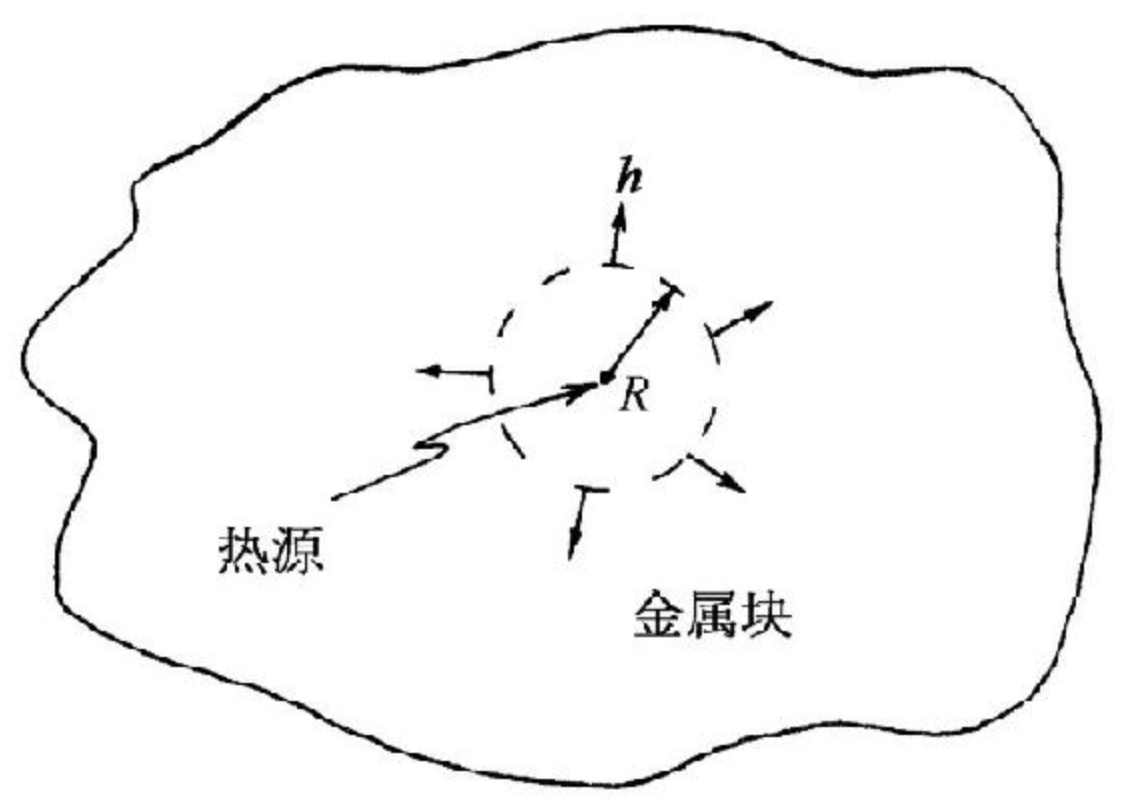
\includegraphics[width=0.3\textwidth]{image/flux.png}
  \end{center}
    \caption{小正方形环积分}
    \label{fig:closurface}
\end{wrapfigure}

答案是肯定的。而且这个办法会引出一个贯穿整个电磁学的重要公式：\textbf{高斯公式}，也叫做散度定理。设想一个闭合曲面 $S$，它围出了一个三维区域 $V$。我们想计算电场 $\mathbf{E}$ 穿过这个闭合曲面的\textbf{净流量}——也就是流出去的减去流进来的。

这个净流量，跟区域内部发生的事情密切相关。如果在区域内部的某一点，矢量场像一个小喷泉一样向外发散，那它对净流量的贡献就是正的；如果像一个小漏斗一样向内汇聚，贡献就是负的；如果只是单纯地流过而没有源头或陷阱，贡献就是零。但是我们该怎么描述这个想法呢？

吱吱吱吱吱吱吱吱吱吱吱吱吱吱吱吱吱吱吱吱吱吱吱吱吱吱吱吱吱吱吱吱吱吱吱在

\begin{wrapfigure}{R}{0.32\textwidth}
  \begin{center}
    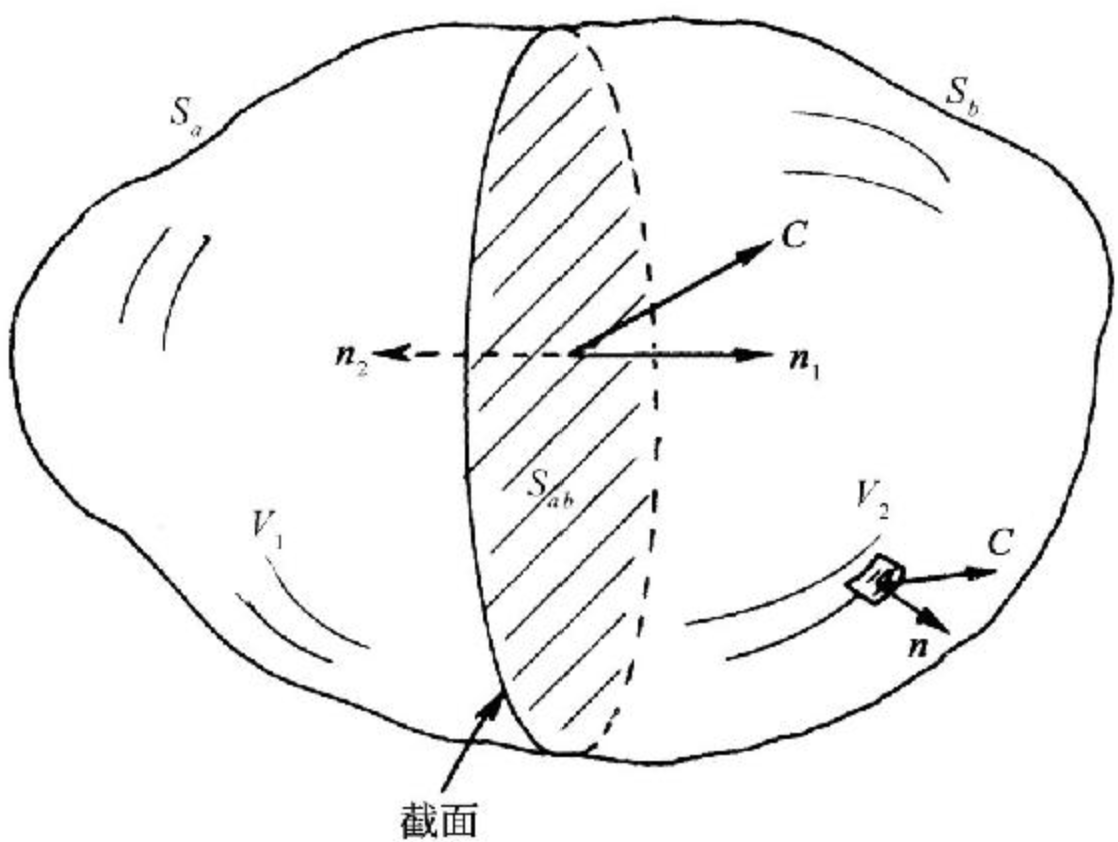
\includegraphics[width=0.3\textwidth]{image/divsurf.png}
  \end{center}
    \caption{小正方形环积分}
    \label{fig:closurface}
\end{wrapfigure}

我们把这个闭合的三维区域切成两块，比如分成 $V_1$ 和 $V_2$，它们的边界曲面分别是 $S_1$ 和 $S_2$，而公共截面则出现了两次。这时，一个绝妙的抵消发生了——在公共截面上，$S_1$ 的外法向与 $S_2$ 的外法向恰好相反，因此分别计算 $S_1$ 和 $S_2$ 上的通量再相加时，截面的贡献正好一正一负，爽快地抵消为零。剩下的部分拼起来，恰好就是原来那个闭合曲面 $S$ 上的总通量。所以说，先分割再求和，与直接对整个 $S$ 积分，结果完全一样。于是乎，我们就可以把任意一个复杂的三维体切割成无数个小正方体来讨论。吱吱吱吱吱吱吱吱吱吱吱吱吱吱吱吱吱吱吱吱吱吱吱吱吱吱吱吱吱吱吱吱吱吱吱吱吱吱吱吱吱吱吱在
\begin{wrapfigure}{L}{0.32\textwidth}
  \begin{center}
    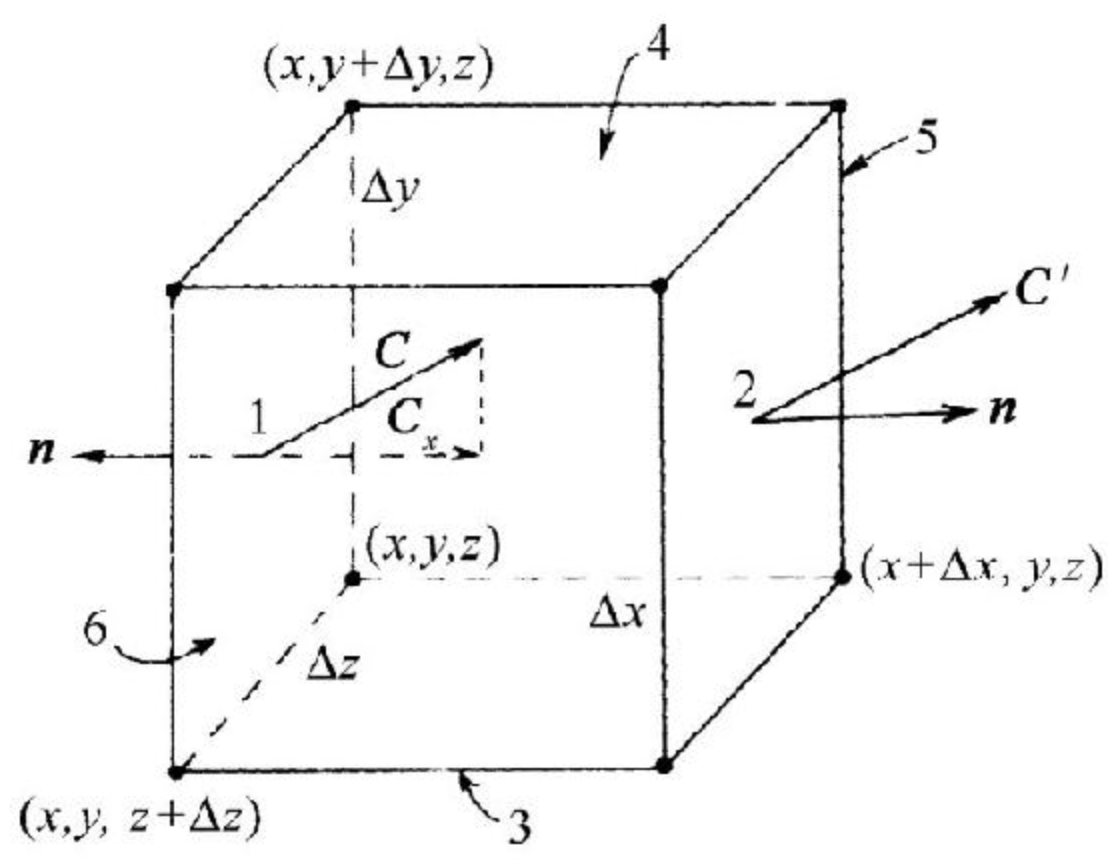
\includegraphics[width=0.3\textwidth]{image/suqflux.png}
  \end{center}
    \caption{小正方形环积分}
    \label{fig:closurface}
    \vspace{10pt}
\end{wrapfigure}


考虑三个方向是对称的，所以我们以 $x$ 方向为例。对于矢量场 $\mathbf{C}$ 在面1和面2上的通量，就是：
\[
\mathbf{C}(x+\Delta x,y,z) \cdot \mathbf{n}\,\Delta y \Delta z \;+\; \mathbf{C}(x,y,z) \cdot (-\mathbf{n}\,\Delta y \Delta z).
\]
这个式子，是不是像之前一样，可以稍稍改写？
\[
\mathbf{C}(x+\Delta x,y,z) - \mathbf{C}(x,y,z) = \frac{\partial \mathbf{C}}{\partial x}\,\Delta x.
\]
于是，$x$ 方向上一对相对面贡献的净通量约为 
\[
\frac{\partial C_x}{\partial x}\,\Delta x \Delta y \Delta z.
\]
同理，$y$ 方向和 $z$ 方向也给出类似的表达式。把三个方向的贡献加起来，就得到这个小正方体总共的净通量：
\[
\left( \frac{\partial C_x}{\partial x} + \frac{\partial C_y}{\partial y} + \frac{\partial C_z}{\partial z} \right) \Delta V,
\]
其中 $\Delta V = \Delta x \Delta y \Delta z$ 是小正方体的体积。


于是数学家定义了一个叫做\textbf{散度}的量，记作 $\nabla \cdot \mathbf{E}$。它是一个\textbf{标量场}，在每一点上的数值可以理解为：\emph{围绕该点取一个无穷小的体积，测量穿过这个小体积边界的净流量，再除以这个微小体积。}换句话说，散度就是“单位体积的净流出量”。

把上面这个小正方体的结果，对全部分割的小体求和，所有内部截面上的通量都会因为相邻小体法向相反而是相互抵消（就像格林公式中内部线段上的抵消一样），只剩下最外层边界曲面 $S$ 上的总通量。于是我们就得到了高斯公式：

\[
\iint_{S}
\left[
\frac{1}{4\pi\varepsilon_0}
\iiint_{V'}
\rho\,
\frac{\hat{\mathbf R}}{R^2}\,
dV
\right]
\cdot d\mathbf S
=
\iiint_{V}
(\nabla\cdot \mathbf E)\,
dV
\]

左边是矢量场穿过闭合曲面 $S$ 的净流量（边界上的总和），右边是散度在内部区域 $V$ 上的三重积分（内部源头强度的总和）。

“散度”这个名字起得极其贴切。如果 $\nabla \cdot \mathbf{A} > 0$，表示该点是“源”，流体从这里\textbf{散}发出去；如果 $\nabla \cdot \mathbf{A} < 0$，表示该点是“汇”，流体向这里\textbf{汇聚}；如果 $\nabla \cdot \mathbf{A} = 0$，表示该点没有源头也没有陷阱，流进来的和流出去的一样多，也就是\textbf{无源场}（比如磁场）。

接下来我们把这个公式套到点电荷场上，我们得到：
\[
\iint_{S} \mathbf{E} \cdot d\mathbf{S} = \iint_{S} \mathbf{E} \cdot d\mathbf{S} = \iiint_{V} (\nabla \cdot \mathbf{E}) \, dV.
\]
高斯通量定理给出电场通量与包围电荷的关系。真空中的积分形式为
\[
\oint_S \vec E\cdot d\vec S = \frac{Q_{\rm enc}}{\varepsilon_0},
\qquad Q_{\rm enc}=\int_V \rho\,dV.
\]
微分形式为
\[
\nabla\cdot\vec E=\frac{\rho}{\varepsilon_0}.
\]
若存在介质，引入电位移矢量
\[
\vec D=\varepsilon_0\vec E+\vec P,
\]
则有
\[
\oint_S \vec D\cdot d\vec S=Q_{\rm free},
\qquad \nabla\cdot\vec D=\rho_{\rm free}.
\]
在线性各向同性介质中，
\[
\vec D=\varepsilon\vec E=\varepsilon_r\varepsilon_0\vec E.
\]

高斯定理本身对任意闭合曲面成立，但只有在高对称性下才便于直接求场。典型模型如下。

\subsubsection{模型一：无限长均匀带电直线}

设无限长直线电荷密度为 $\lambda$。取半径为 $r$、长为 $L$ 的同轴圆柱面为高斯面。由轴对称性，电场沿径向，且在同一圆柱面上大小相等。上下底面通量为零，侧面通量为
\[
\Phi_E=E(r)\cdot 2\pi r L.
\]
包围电荷为
\[
Q_{\rm enc}=\lambda L.
\]
由高斯定理
\[
E(r)\cdot 2\pi r L=\frac{\lambda L}{\varepsilon_0},
\]
故
\[
E(r)=\frac{\lambda}{2\pi\varepsilon_0 r},
\qquad
\vec E=\frac{\lambda}{2\pi\varepsilon_0 \rho}\hat{\rho}.
\]
若带电体是半径为 $R$ 的无限长导体圆柱，则外部场同上，内部场为零，表面电荷密度满足
\[
\sigma=\frac{\lambda}{2\pi R}.
\]

\subsubsection{模型二：无限大均匀带电薄板}

设无限大薄板面电荷密度为 $\sigma$。取一个穿过薄板、底面积为 $A$ 的圆柱形高斯面，两底面平行于薄板。由平面对称性，电场垂直薄板，两侧大小相等、方向相反。两底面通量为
\[
\Phi_E=2E A.
\]
包围电荷为
\[
Q_{\rm enc}=\sigma A.
\]
于是
\[
2E A=\frac{\sigma A}{\varepsilon_0},
\qquad
E=\frac{\sigma}{2\varepsilon_0}.
\]
方向为正电荷两侧远离薄板：
\[
\vec E=
\begin{cases}
\dfrac{\sigma}{2\varepsilon_0}\hat n, & \text{板外侧正法向一侧},\\[6pt]
-\dfrac{\sigma}{2\varepsilon_0}\hat n, & \text{板外侧负法向一侧}.
\end{cases}
\]
若薄板为无限大导体板，总面电荷密度为 $\sigma$，电荷分布在两个表面上，每面约为 $\sigma/2$，板外电场大小仍为
\[
E=\frac{\sigma}{2\varepsilon_0},
\]
板内电场为零。

\subsection{附：通电直导线的磁场与安培环路定理}

需要注意：高斯通量定理处理的是电场。若模型是“通电导线”，应使用磁场高斯定理和安培环路定理：
\[
\oint_S \vec B\cdot d\vec S=0,
\qquad \nabla\cdot\vec B=0,
\]
\[
\oint_C \vec B\cdot d\vec l=\mu_0 I_{\rm enc},
\qquad \nabla\times\vec B=\mu_0\vec J.
\]
对于无限长直导线，电流为 $I$。取半径为 $\rho$ 的同轴圆形回路，由轴对称性
\[
B(\rho)\cdot 2\pi \rho=\mu_0 I,
\]
故
\[
B(\rho)=\frac{\mu_0 I}{2\pi \rho},
\qquad
\vec B=\frac{\mu_0 I}{2\pi \rho}\hat{\phi},
\]
方向满足右手螺旋定则。若导线半径为 $R$ 且电流均匀分布，则
\[
B(\rho)=
\begin{cases}
\dfrac{\mu_0 I \rho}{2\pi R^2}, & \rho<R,\\[8pt]
\dfrac{\mu_0 I}{2\pi \rho}, & \rho>R.
\end{cases}
\]

\section{量子电动力学的拉格朗日密度}

本章从自由狄拉克场的全局 $U(1)$ 对称性出发，考察这一对称性由全局推广到局域时所遇到的困难；为了恢复不变性，我们被迫在微分算子中引入一个新的场 $A_{\mu}$，并由此确定它的变换规则与协变导数 $D_{\mu}$。最后我们构造出与 $\partial_{\mu}A_{\nu}$ 有关的规范不变组合，即场强张量，从而得到量子电动力学的拉格朗日密度。

\subsection{全局对称性与守恒律}

首先我们写出自由狄拉克拉格朗日密度：
\[
\mathcal{L}_{\text{free}}=\overline{\psi}\left( i\gamma^{\mu}\partial_{\mu}-m \right)\psi
\]
其中狄拉克共轭为：$\overline{\psi}=\psi^{\dagger}\gamma^{0}$，它表示转置并取复共轭。

然后我们对旋量做一个全局变换：
\[
\psi(x)\to\psi'(x)=e^{iq\theta}\psi(x)
\]
\[
\overline{\psi}(x)\to\overline{\psi}'(x)=e^{-iq\theta}\overline{\psi}(x)
\]
带入到我们的自由狄拉克拉格朗日密度中：
\[
\left\{
\begin{aligned}
\mathcal{L}_{\text{free}}' &= \overline{\psi}'\left( i\gamma^{\mu}\partial_{\mu}-m \right)\psi'
=\left( e^{-iq\theta}\overline{\psi} \right)\left( i\gamma^{\mu}\partial_{\mu}-m \right)\left( e^{iq\theta}\psi \right)\\
\mathcal{L}_{\text{free}} &= \overline{\psi}\left( i\gamma^{\mu}\partial_{\mu}-m \right)\psi
\end{aligned}
\right.
\]
不难看出自由狄拉克拉格朗日密度在全局 $U(1)$ 变换下是不变的，根据诺特定理，这个连续的全局对称性对应一个守恒流。守恒流为：
\[
j^{\mu}=q\overline{\psi}\gamma^{\mu}\psi
\]
可以验证 $\partial_{\mu}j^{\mu}=0$，即电荷守恒。

\subsection{局域对称性破缺与规范场}

那么现在我们对每一个坐标点定义一个变换 $\chi(x)$，于是局域变换可以写作：
\[
\left\{
\begin{aligned}
\psi(x) &\to \psi'(x)=e^{iq\chi(x)}\psi(x)\\
\overline{\psi}(x) &\to \overline{\psi}'(x)=e^{-iq\chi(x)}\overline{\psi}(x)
\end{aligned}
\right.
\]
现在我们计算变换后的自由拉格朗日密度：
\[
\mathcal{L}_{\text{free}}'=\overline{\psi}'\left( i\gamma^{\mu}\partial_{\mu}-m \right)\psi'
=\left( e^{-iq\chi}\overline{\psi} \right)\left( i\gamma^{\mu}\partial_{\mu}-m \right)\left( e^{iq\chi}\psi \right)
\]
其中 $\partial_{\mu}\left( e^{iq\chi}\psi \right)=e^{iq\chi}\partial_{\mu}\psi+iq\left( \partial_{\mu}\chi \right)e^{iq\chi}\psi$，于是：
\[
\mathcal{L}_{\text{free}}'=e^{-iq\chi}\overline{\psi}\left[ i\gamma^{\mu}\left( e^{iq\chi}\partial_{\mu}\psi+iq\left( \partial_{\mu}\chi \right)e^{iq\chi}\psi \right)-me^{iq\chi}\psi \right]
\]
\[
=\overline{\psi}\left[ i\gamma^{\mu}\left( \partial_{\mu}\psi+iq\left( \partial_{\mu}\chi \right)\psi \right)-m\psi \right]
\]
\[
=\overline{\psi}\left( i\gamma^{\mu}\partial_{\mu}-m \right)\psi+\overline{\psi}\left[ i\gamma^{\mu}\left( iq\left( \partial_{\mu}\chi \right) \right)\psi \right]
\]
\[
=\mathcal{L}_{\text{free}}-q\left( \partial_{\mu}\chi \right)\left( \overline{\psi}\gamma^{\mu}\psi \right)
\]
那么我们得到：
\[
\mathcal{L}_{\text{free}}'=\mathcal{L}_{\text{free}}-\left( \partial_{\mu}\chi \right)j^{\mu}
\]
其中 $j^{\mu}$ 就是前面找到的守恒流。

为了消除多出来的项，我们在微分算子中新引入一个场，即协变导数
\[
D_{\mu}\psi=\left( \partial_{\mu}+iqA_{\mu} \right)\psi
\]
这个新引入的场 $A_{\mu}$ 的行为尚未确定，所以我们的目标是：设计 $A_{\mu}$ 的变换规则，使得 $D_{\mu}\psi$ 和 $\psi$ 本身以相同的方式变换即“协变”：
\[
\left( D_{\mu}\psi \right)'=e^{iq\chi}\left( D_{\mu}\psi \right)
\]
我们分别展开左右两侧得到：
\[
\left\{
\begin{aligned}
\left( D_{\mu}\psi \right)' &= e^{iq\chi}\left[ \partial_{\mu}\psi+iq\left( \partial_{\mu}\chi \right)\psi+iqA_{\mu}'\psi \right]\\
e^{iq\chi}\left( D_{\mu}\psi \right) &= e^{iq\chi}\left( \partial_{\mu}\psi+iqA_{\mu}\psi \right)
\end{aligned}
\right.
\]
\[
\Rightarrow \partial_{\mu}\psi+iq\left( \partial_{\mu}\chi \right)\psi+iqA_{\mu}'\psi=\partial_{\mu}\psi+iqA_{\mu}
\]
也就是说最后得到的场要求：
\[
A_{\mu}'+\partial_{\mu}\chi=A_{\mu}
\]
场 $A_{\mu}$ 的变换满足：
\[
\boxed{A_{\mu}\to A_{\mu}'=A_{\mu}-\partial_{\mu}\chi}
\]
于是我们耦合后的拉格朗日密度可以写为：
\[
\mathcal{L}_{\text{matter}}=\overline{\psi}\left( i\gamma^{\mu}D_{\mu}-m \right)\psi
\]
展开后不难看出各项的物理意义：
\[
\mathcal{L}_{\text{matter}}
=\underbrace{\overline{\psi}\left( i\gamma^{\mu}\partial_{\mu}-m \right)\psi}_{\mathcal{L}_{\text{free}}}
\underbrace{-qA_{\mu}\left( \overline{\psi}\gamma^{\mu}\psi \right)}_{\text{相互作用项}-A_{\mu}j^{\mu}}
\]
我们不难验证新的拉格朗日密度在局域变换下不变：
\[
\mathcal{L}_{\text{matter}}'=\mathcal{L}_{\text{matter}}
\]

\subsection{构造规范场的动力学项}

我们有了符合要求的场，但我们并不确定其动力学意义是怎样的，从上面的推导我们知道
\[
\partial_{\mu}A_{\nu}'=\partial_{\mu}\left( A_{\nu}-\partial_{\nu}\chi \right)=\partial_{\mu}A_{\nu}-\partial_{\mu}\partial_{\nu}\chi
\]
我们需要构造一个与 $\partial_{\mu}A_{\nu}$ 相关的、规范不变的组合。

考虑 $D_{\mu}$ 的对易子：
\[
\left[ D_{\mu},D_{\nu} \right]\psi=D_{\mu}\left( D_{\nu}\psi \right)-D_{\nu}\left( D_{\mu}\psi \right)
\]
计算这个对易子可以发现，所有关于 $\psi$ 的导数项 $\partial_{\mu}\psi$ 和 $\partial_{\nu}\partial_{\mu}\psi$ 都抵消了，$A_{\mu}A_{\nu}$ 项也因为对称性而抵消。

最终结果是：
\[
\left[ D_{\mu},D_{\nu} \right]\psi=iq\left( \partial_{\mu}A_{\nu}-\partial_{\nu}A_{\mu} \right)
\]
我们定义场强张量：
\[
\boxed{F_{\mu\nu}=\partial_{\mu}A_{\nu}-\partial_{\nu}A_{\mu}}
\]
所以：
\[
\left[ D_{\mu},D_{\nu} \right]\psi=iqF_{\mu\nu}
\]
因而拉格朗日密度动力学项可以写为：
\[
\mathcal{L}=\frac{1}{4}F^{\mu\nu}F_{\mu\nu}
\]
所以电动力学规范理论拉格朗日密度：
\[
\mathcal{L}_{QED}
=\underbrace{\overline{\psi}\left( i\gamma^{\mu}\partial_{\mu}-m \right)\psi}_{\text{自由电子场}}
\underbrace{-qA_{\mu}\left( \overline{\psi}\gamma^{\mu}\psi \right)}_{\text{电子与光子的相互作用}}
\underbrace{-\frac{1}{4}F^{\mu\nu}F_{\mu\nu}}_{\text{自由电磁场（光子）}}
\]
用狄拉克算符简写作：
\[
\boxed{\mathcal{L}_{QED}
=\underbrace{\overline{\psi}\left( i\gamma^{\mu}D_{\mu}-m \right)\psi}_{\text{自由电子场}}
\underbrace{-\frac{1}{4}F^{\mu\nu}F_{\mu\nu}}_{\text{自由电磁场（光子）}}}
\]

\end{document}